% !TEX program = xelatex
\documentclass[11pt,a4paper]{article}

% This template uses parts inspired by the
% template created by DAndexer & SEntacher

%\usepackage{utf8}{inputenc}
% For Umlaute and special characters
%\usepackage[ngerman]{babel}
% Page margins etc.
\usepackage[a4paper]{geometry}
% Set font
\usepackage{fontspec}
% Using images
\usepackage{graphicx}
% Easier quoting
\usepackage{csquotes}
% Customized headers and footers
\usepackage{fancyhdr}
% Make clickable toc and more
\usepackage{hyperref}
\hypersetup{
    pdftitle={On the Predictability of Remission in Colorectal Tumor Patients using Radiomics},
    pdfsubject={Testing the Predictability of Remission in Colorectal Tumor Patients using Radiomics},
    pdfauthor={Valentin Schweitzer},
    pdfkeywords={pCR, Radiomics, Colorectal Tumors, Random Forests, Bachelor Thesis},
    colorlinks,
    citecolor=black,
    filecolor=black,
    linkcolor=black,
    urlcolor=black
}
% For re-using \author and co.
\usepackage{titling}
\author{Valentin Schweitzer}
\date{\today}
\title{On the Predictability of Remission in\\Colorectal Tumor Patients using Radiomics}

% For displaying/referencing section names
\usepackage{nameref}
\makeatletter
%\newcommand*{\currentname}{\@currentlabelname}
\newcommand*{\currentname}{\leftmark}

\makeatother

% Subfigures
\usepackage{subcaption}
% Schmemata and drawings
\usepackage{tikz}
\usetikzlibrary{matrix,fit,calc,positioning,chains,shapes.multipart}
% Better figure positioning
\usepackage{float}
% Better tables
\usepackage{tabularx}
% Long tabularx tables
\usepackage{xltabular}
% Generate filler text
\usepackage{kantlipsum}
% Glossary and acronyms
\usepackage{acronym}
% Easier tree drawing
\usepackage{tikz-qtree}
% Stuff like math letters
\usepackage{amsfonts}

\usepackage{pgf-umlcd}

% Taken from https://tex.stackexchange.com/questions/416466/acronym-package-handling-possessive-case-apostrophe-s
\makeatletter
\newcommand{\acg}[1]{%
    \expandafter\ifx\csname AC@#1\endcsname\AC@used
        \acs{#1}'s%
    \else
        \aclu{#1}'s (\acs{#1})%
    \fi
}
\makeatother

\makeatletter
\newcommand{\acsg}[1]{%
    \acs{#1}'s%
}
\makeatother

% Number Reference section
\usepackage{tocbibind}
% Change the date format
\usepackage{datetime2}
% Change width of figure captions
\usepackage{caption}
% Set global caption width
\captionsetup{width=12cm}
\usepackage{enumitem}

\usepackage{forest}

% Bibliography management
\usepackage[
    minnames=6,
    maxnames=6,
    style=ieee,
    dateabbrev=false,
    citestyle=numeric-comp
]{biblatex}

\addbibresource{bib.bib}

%\def\citepunt{,\,}

% Uncomment for better font
% \setmainfont{Comic Sans MS}

% Load custom fonts if available
\IfFontExistsTF{Crimson Pro}{
    \setmainfont[
        BoldFont={Crimson Pro Medium},
        ItalicFont={Crimson Pro Light Italic},
        LetterSpace = -2 % Move letters slightly closer together
    ]{Crimson Pro Light}
}{
    % Use font files
    \setmainfont[
        ExternalLocation={fonts/},
        BoldFont={CrimsonPro-Medium.ttf},
        ItalicFont={CrimsonPro-LightItalic.ttf},
        LetterSpace = -2 % Move letters slightly closer together
    ]{CrimsonPro-Light.ttf}
}
\IfFontExistsTF{Space Mono}{
    \setmonofont[
        BoldFont={Space Mono Bold},
        ItalicFont={Space Mono Italic},
        LetterSpace = -4, % Move letters slightly closer together
        Scale=0.8
    ]{Space Mono}
}{
    \setmonofont[
        ExternalLocation={fonts/},
        BoldFont={SpaceMono-Bold.ttf},
        ItalicFont={SpaceMono-Italic.ttf},
        Scale=0.8,
        LetterSpace = -4 % Move letters slightly closer together
    ]{SpaceMono-Regular.ttf}
}

% Used to enquote stuff
\usepackage{csquotes}
% For equations
\usepackage{mathtools}
% For code blocks
\usepackage{listings}
\usepackage{color}
% https://en.wikibooks.org/wiki/LaTeX/Source_Code_Listings
\definecolor{mygreen}{rgb}{0,0.6,0}
\definecolor{mygray}{rgb}{0.5,0.5,0.5}
\definecolor{mymauve}{rgb}{0.58,0,0.82}

\lstset{
    basicstyle=\ttfamily\footnotesize,
    breakatwhitespace=false,         
    breaklines=false,                 
    captionpos=b,                    
    keepspaces=true,                 
    numbers=left,                    
    numbersep=0pt,             
    numberstyle=\ttfamily\footnotesize,
    showspaces=false,                
    showstringspaces=false,
    showtabs=false,                  
    tabsize=4
}

\usepackage{caption}
\captionsetup[table]{skip=14pt}
% Support for multi-page tables
\usepackage{longtable}

% Support for column-text
\usepackage{multicol}

% For tikz plots
\usepackage{pgfplots}
\usepgfplotslibrary{fillbetween}

% Number representations
\usepackage{siunitx}

% Group (put space inbetween pairs of 3) only integers
\sisetup{
    group-digits=integer,
    round-mode=figures,
    round-precision=3, 
    inter-unit-product=\ensuremath{{\cdot}},
    output-product=\ensuremath{\cdot},
    exponent-product=\ensuremath{\cdot},
    detect-all,
}

% Control footnote indent
\usepackage[hang,flushmargin]{footmisc} 

% Fix paragraph spacing
\setlength{\parindent}{0em}
\setlength{\parskip}{1em}

% Short hyphen for use in math mode
\mathchardef\mhyphen="2D

%%%%%%%%%%%%%%%%%%%%
% Custom variables %
%%%%%%%%%%%%%%%%%%%%

\newcommand{\threeDcount}{7}
\newcommand{\removelinebreaks}[1]{%
      \def\\{ }#1}

\newcommand{\tbd}{\begin{center}\dots\textit{TBD}\dots\end{center}}
\newcommand{\featureCount}{1743}

% https://tex.stackexchange.com/questions/215697/skip-line-numbers-and-resume-from-specific-number

\newcommand*\Suppressnumber{%
  \lst@AddToHook{OnNewLine}{%
    \let\thelstnumber\relax%
     \advance\c@lstnumber-\@ne\relax%
    }%
}

\newcommand*\Reactivatenumber{%
  \lst@AddToHook{OnNewLine}{%
   \let\thelstnumber\origthelstnumber%
   \advance\c@lstnumber\@ne\relax}%
}

% https://tex.stackexchange.com/questions/89166/centering-in-tabularx-and-x-columns
\newcolumntype{Y}{>{\centering\arraybackslash}X}

\listfiles

\begin{document}
% !TEX program = xelatex

\newgeometry{top=2cm,right=2cm,bottom=2cm,left=2cm}
\pagenumbering{gobble}
\begin{center}
\vspace{0cm}
\includegraphics{./img/fhs_logo.jpg}\par
\vspace{1cm}
{\addfontfeature{LetterSpace=5.0}
    {\LARGE BACHELOR THESIS\par}
}
\vspace{1cm}
{\Large \textbf{\thetitle}\par}
\vspace{2.5cm}
submitted to the course of\\
Information Technology and Systems Management\\
Salzburg University of Applied Sciences\par
\vspace{2.5cm}
submitted by\\
\textbf{\theauthor}\par
\vspace{2.5cm}

\begin{tabular}{lr}
    Head of school: & FH-Prof.\ DI Dr.\ Gerhard Jöchtl\\
    Supervisor: & FH-Prof.\ Dr.\ Michael Gadermayr\\
\end{tabular}
\par
\vfill
Puch, on \today
\end{center}
\restoregeometry

\newgeometry{top=2.5cm,right=2.5cm,bottom=3cm,left=2.5cm}
\pagenumbering{roman}
\setlength{\headheight}{15pt}
\pagestyle{fancy}
\fancyhf{}
\rhead{\thepage}
% !TEX program = xelatex
\section*{Declaration on oath}
I hereby declare on oath that I have written this
bachelor’s thesis on my own and without
external assistance, and have used no other source
materials or aids than those listed. Furthermore,
I hereby affirm that I have identified any text or
content taken from the source materials used accordingly.

To date, this paper has neither been submitted to any
other examination board, in this country or abroad,
nor published in an identical or similar form.

\vspace{1.5cm}
\begin{tabular}{p{0.3\textwidth} m{0.35\textwidth} p{0.3\textwidth}}
    \underline{\today} & & \rule{0.25\textwidth}{0.01cm}\hspace{-0.25\textwidth}\includegraphics[width=2cm]{img/signature.png}\\
    Date               & & Signature
\end{tabular}
\newpage
% !TEX program = xelatex
\section*{Acknowledgements}

% I would sincerely like to thank ISO/IEC 14496-12:2015(E)
% Annex F for reminding me that you do not have to be
% useful to be published in an ISO/IEC standard.

% Draft 2:
I would like to thank everyone who so patiently helped me in writing this 
thesis.

This thesis would not have been possible without those that provided open access
to their work and knowledge.
\newpage
\section*{Abstract}

\paragraph{Purpose} To determine the predictability of \acs{pcr} in colorectal
tumor patients using statistical properties of associated \acs{mri} imaging data.
Through the usage of a standardized radiomics library, beneficial radiomics 
features for a better-than-random classification performance are determined. 
The implementation of this setup is attempted through the sole use
of widely available or replicable tools.

\paragraph{Experimental Setup} The dataset featuring inconsistent tumor annotations
was processed by a common semi-automatic annotation algorithm. An initial count 
of \featureCount{} radiomics features was extracted using PyRadiomics. Each 
feature was then assigned a weighted \enquote{importance} score, depending on 
its contribution to a successful classification. Finally, the ideal importance 
threshold was determined.

Additionally, the possibility of favorable feature combinations was explored by
creating groupings of related features. Models based on those groupings were
evaluated by comparing their actual performance against their expected 
performance. Feature combinations performing unexpectedly well were marked as 
potentially beneficial in combination.

Model performance was evaluated using a combination of balanced accuracy and 
\acs{roc} curve metrics. Measures were taken over the average of 100 classifier
models for any set of parameters.

\paragraph{Results} A classifier model reaching a balanced
accuracy of \num{0.697142857142857} (\SI{95}{\percent} Confidence Interval 
[\num{0.68272882292878}, \num{0.711556891356934}]) and an AUC mean of 
\num{0.766326530612245} (\SI{95}{\percent} Confidence Interval:
[\num{0.7529118302973336}, \num{0.7797412309271564}]) has been constructed.

Favorable groupings for increased model accuracy have been found.

\paragraph{Conclusion} In concordance with similar studies, the prediction of 
\acs{pcr} in colorectal tumor patients based on radiomics features seems 
possible.

Studies utilizing a different classification model for comparable challenges 
consistently performed better than the \acs{rf}-based classifier used here. 
Along with a strong difference in the amount of selected features, this result
possibly calls the effectiveness of the feature selection algorithm introduced 
in this thesis into question.

Although feature groupings that perform unusually well together have been found
as expected, low correlation between expected and achieved grouping performance
points to flaws in either the evaluation of groupings or the earlier mentioned 
weighting of feature importances.
% !TEX program = xelatex
\tableofcontents
% \listoffigures
% \listoftables
% Add chapter name with content
%\lhead{\removelinebreaks{\thetitle}}
\lhead{\currentname}
\pagenumbering{arabic}
\section{Introduction}

This section gives an overview about the reasoning behind the creation of this 
thesis, along with a comparison of similar studies. For a practically oriented overview of this thesis, refer to Figure~\ref{fig:graphical_overview}.

\subsection{Motivation}

Cancer is one of the leading causes of death in adults worldwide. Estimated to
be the third most diagnosed type of cancer in 2020, colorectal cancer is both 
common and carries a high mortality rate~\cite{cancer_stats_2020}. The response to treatment varies 
between patients, where complete recovery is known as \acf{pcr}~\cite{Zorcolo2012}.
The prediction of \ac{pcr} aides in the choice of treatment of patients suffering
from tumors~\cite{radiomics_analysis_pcr_rectal}. Although this prediction has 
been the aim multiple studies, the methodology used is often difficult to 
reproduce, through the use of either undocumented or non-standard
implementations. 

\subsection{Aim of this Thesis}

The aim of this thesis is to investigate a connection between statistical 
features of common \ac{mri} images and the \ac{pcr} of a patient.
A radiomics-based
machine learning model in the shape of \iac{rf}-based classifier, will be used 
in an attempt to predict \ac{pcr} in 
colorectal tumor patients significantly better than trough random choice.
To improve reproducibility, publicly accessible and well-document tools will be 
used. Where applicable, the idea behind custom implementations and their mode
of operation shall be well-described, in order to be easily replicated.


\subsection{State of Research}\label{sec:state_of_research}

Numerous papers have been written about the analysis of tumors using radiomics,
though the focus on colorectal tumors is comparatively sparse. As of time of 
writing, three other papers are known to focus on the prediction 
of \ac{pcr} via radiomics features extracted from \ac{mri} scans of rectal 
tumors~\cite{radiomics_analysis_pcr_rectal,rectal_radiomics_svm_rf,multisite_rectal_radiomics}.
A comparison of methodology and results of these studies is shown in 
Table~\ref{tbl:other_studies_auc}. All three studies were successful in 
separating \ac{pcr} and non-\ac{pcr} patients at a rate better than through 
simple guesses. Two of these studies employed either \iac{rf}-based model, or
one including \iac{rf} classifier.

\begin{table}[H]
    \centering
    \begin{tabular}{c c c c c}
        Study & Patients in Dataset & Classification Model & AUC & \SI{95}{\percent} Confidence Interval \\
        \hline
        \cite{radiomics_analysis_pcr_rectal} & \num{222} & \acs{svm} & \num{0.9756} & [\num{0.9185}, \num{0.9711}] \\
        \cite{rectal_radiomics_svm_rf} & \num{134} & Mixed, including \acs{svm} and \acs{rf} & \num{0.91} & [\num{0.83}, \num{0.98}] \\
        \cite{multisite_rectal_radiomics} & \num{104} & \acs{rf} & \num{0.712} & --- % TODO: Check if Hold-out of Discovery validation should be used TODO: What is the confidence interval?
    \end{tabular}
    \caption{A comparison of studies on the prediction of \ac{pcr} using \ac{mri}-based radiomics features. Where missing, data was not available from the original study.}\label{tbl:other_studies_auc}
\end{table}

Although all datasets
consisted of \ac{mri} imaging data, significant differences in scan 
composition were shown. All studies included T\textsubscript{2} weighted scans, 
with~\cite{radiomics_analysis_pcr_rectal} using additional \ac{dwi} data, where each weighting was recorded at 
two distinct points in time.~\cite{rectal_radiomics_svm_rf} states access to
additional T\textsubscript{1} weighted scans, though it focuses on the analysis 
of T\textsubscript{2} data.

Additionally, selection of \ac{roi} varied in methodology. While all studies 
used manual annotations, \cite{multisite_rectal_radiomics} utilized a combined 
approach of using both the largest available tumor slice and a volumetric 
representation of the entire tumor, while~\cite{rectal_radiomics_svm_rf} 
and~\cite{multisite_rectal_radiomics} opted for the former and latter approaches
respectively.

Although automated and semi-automatic tumor annotation techniques are in 
development, all studies listed in Table~\ref{tbl:other_studies_auc} opted for 
manual annotation. As non-manual annotation technologies are, as of time of 
writing, not clearly standardized, a simple \enquote{a priori} shape-based 
algorithm has been used to semi-automatically create 3-dimensional 
annotations in the context of this thesis~\cite{auto_and_semiauto,semiautomatic_prostate,dl_rectal_segmentation}.

For the extraction of radiomics features, both~\cite{radiomics_analysis_pcr_rectal}
and~\cite{multisite_rectal_radiomics} opted for differing custom implementations
using MATLAB\footnote{The MathWorks, Inc.}, where in both cases a description, 
of varying detail, of the features utilized, was published. In contrast,~\cite{rectal_radiomics_svm_rf} chose MaZda~\cite{mazda},
an image texture analysis toolkit. This shows the common intent of a transparent 
feature definition. Though this helps in increasing
reproducibility~\cite{ibsi_paper,radiomics_process_and_challenges}, two 
out of three studies used MATLAB for feature extraction, 
while~\cite{rectal_radiomics_svm_rf} later relies on MATLAB for classification.
This may hinder availability of the methods described in these studies, as 
MATLAB is, as of time of writing, commercial software~\cite{matlab}.
Additionally, even well-documented custom implementations of radiomics features pose 
problems for the comparison between studies, as addressed by~\cite{ibsi_paper}.
To alleviate problems associated with both inconsistent feature definitions and
the potential unavailability of commercial software, this thesis is based on an 
open-source radiomics library, which largely follows \ac{ibsi} recommendations
for feature definitions.

Although using different sets of features and feature definitions, all studies
shown use at least one common method of selecting features (\ac{lasso}~\cite{lasso}).
Additional commonality arises from the features selected, as feature groups
chosen by each study consist largely of texture-based features, such as 
\ac{collage} and Gray-Level Matrices~\cite{radiomics_analysis_pcr_rectal,rectal_radiomics_svm_rf,multisite_rectal_radiomics,collage}.

As the only known study to utilize an identical classifier setup (a purely 
\ac{rf}-based classifier) for the problem posed in this thesis (predicting \ac{pcr} 
in colorectal tumor patients),~\cite{multisite_rectal_radiomics} employs a 
combination of three feature selection variants. In contrast to these measures, 
a selection method based on the ability of \ac{rf} classifiers to determine the
contribution of individual features to the final classification performance is 
used. The choice of \iac{rf} classifier was based on the strength of such 
models to handle a large amount of features extracted from a relatively small 
sample size~\cite{random_forests_article,random_forests_web}. Indeed, the
number of patients in this study is consistently lower than all similar studies
referenced here (compare Section~\ref{sec:materials_dataset} and 
Table~\ref{tbl:other_studies_auc}).


% https://www.bu.edu/math/files/2013/08/tikzpgfmanual.pdf
% https://tex.stackexchange.com/questions/488983/tikz-style-for-rectangle-with-text-in-border
\begin{figure}[H]
    \centering
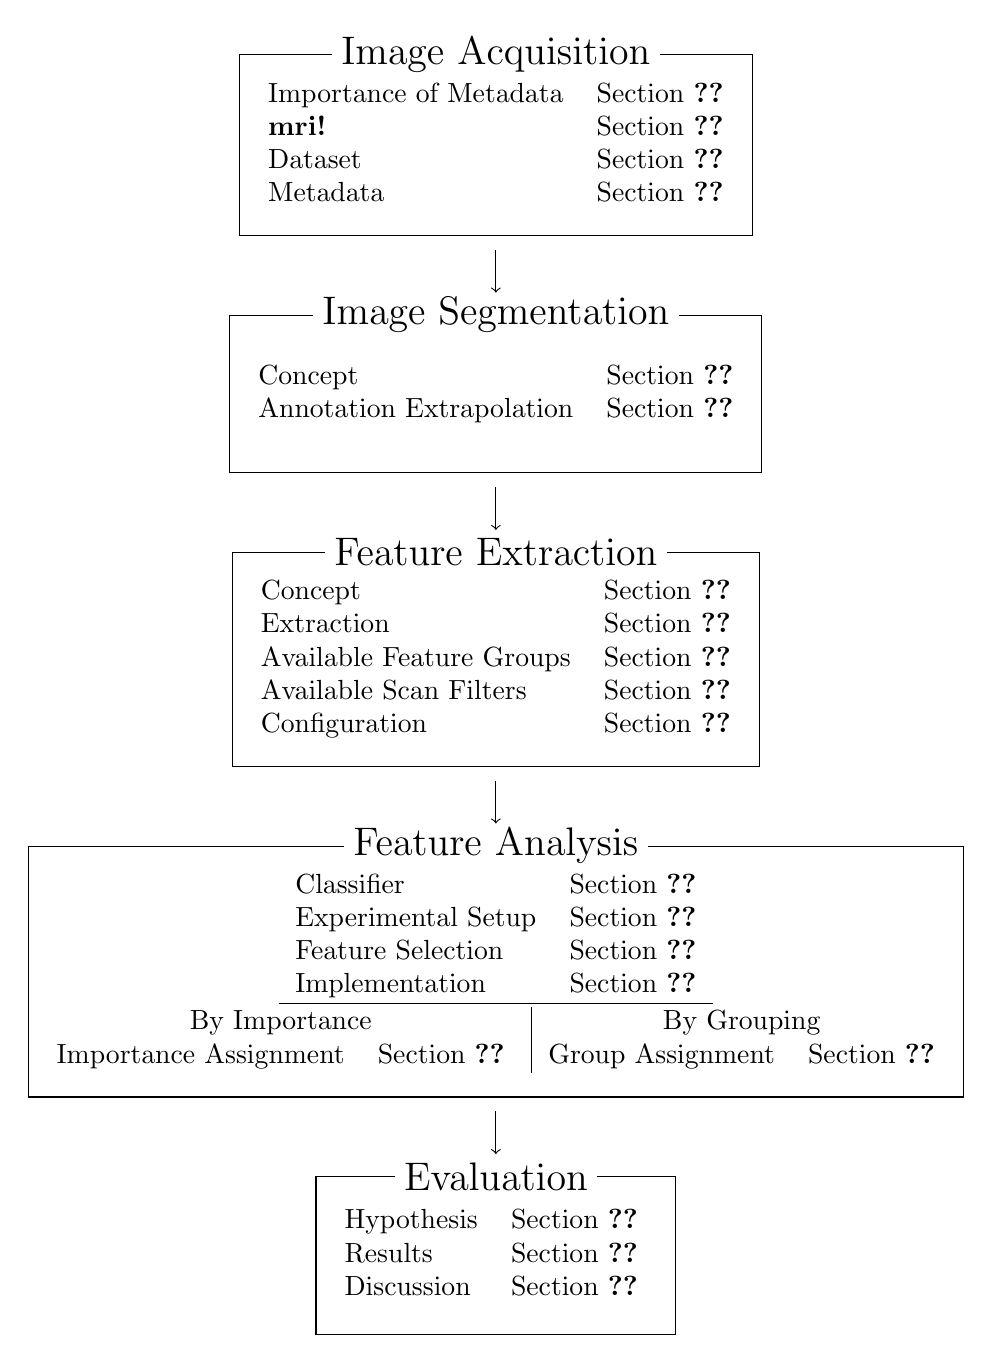
\begin{tikzpicture}[titlerect/.style={draw,inner ysep=2ex,inner
    xsep=1ex,minimum height = 2cm, minimum width={2*width("#1")},align=center,label={[anchor=center,fill=white,font=\Large]above:#1}}]


    \node (img_acq) [titlerect={Image Acquisition}] at (0,0) {\begin{tabular}{l r}
        Importance of Metadata & Section~\ref{sec:radiomics_image_acquisition} \\ 
        \acs{mri} & Section~\ref{sec:intro_mri}\\
        Dataset & Section~\ref{sec:materials_dataset}\\
        Metadata & Section~\ref{sec:mri_metadata} \\
    \end{tabular}};

    \node (img_seg) [below = of img_acq, titlerect={Image Segmentation}] {\begin{tabular}{l r}
        Concept & Section~\ref{sec:radiomics_image_segmentation} \\
        Annotation Extrapolation & Section~\ref{sec:3d_and_2d} \\
    \end{tabular}};

    \node (ftr_ext) [below = of img_seg, titlerect={Feature Extraction}] {\begin{tabular}{l r}
        Concept & Section~\ref{sec:radiomics_feature_extraction} \\
        Extraction & Section~\ref{sec:feature_extraction} \\
        Available Feature Groups & Section~\ref{sec:radiomics_features} \\
        Available Scan Filters & Section~\ref{sec:base_scan_filters} \\
        Configuration & Section~\ref{sec:pyrad_config} \\
    \end{tabular}};

    \node (ftr_als) [below = of ftr_ext, titlerect={Feature Analysis}] {
        \begin{tabular}{l r}
            Classifier & Section~\ref{sec:intro_classification} \\
            Experimental Setup & Section~\ref{sec:experimental_setup} \\
            Feature Selection & Section~\ref{sec:feature_filtering} \\
            Implementation & Section~\ref{sec:code_structure} \\
            \hline
        \end{tabular}

        \\

        \begin{tabular}{l r}
            \multicolumn{2}{c}{By Importance} \\
            Importance Assignment & Section~\ref{sec:filtering_importance} \\
        \end{tabular}
        \vline
        \begin{tabular}{l r}
            \multicolumn{2}{c}{By Grouping} \\
            Group Assignment & Section~\ref{sec:filtering_grouping} \\
        \end{tabular}
    };

    \node (eval) [below = of ftr_als, titlerect={Evaluation}] {
        \begin{tabular}{l r}
            Hypothesis & Section~\ref{sec:hypothesis}\\
            Results & Section~\ref{sec:results}\\
            Discussion & Section~\ref{sec:discussion}\\
        \end{tabular}
    };


    \draw [->, shorten <= 5pt, shorten >= 8pt] (img_acq.south) -- (img_seg.north);
    \draw [->, shorten <= 5pt, shorten >= 8pt] (img_seg.south) -- (ftr_ext.north);
    \draw [->, shorten <= 5pt, shorten >= 8pt] (ftr_ext.south) -- (ftr_als.north);
    \draw [->, shorten <= 5pt, shorten >= 8pt] (ftr_als.south) -- (eval.north);

\end{tikzpicture}
\caption{A rough overview of the sections that make up the central experiment this thesis covers. A summary of this setup is provided in Section~\ref{sec:experimental_setup}.}\label{fig:graphical_overview}
\end{figure}


\newpage{}
\section{Underlying Concepts}

This section gives an overview of concepts that form the base of this 
experimental setup. First, radiomics is described in more detail in 
Section~\ref{sec:intro_radiomics}, along with the imaging technology whose 
results it analyzes, which is examined in Section~\ref{sec:intro_mri}. Second, 
the classification model used here and its evaluation are covered in 
Section~\ref{sec:intro_classification}.

% Maybe break up these sentences^

% "Graphical Overview".
% Not sure how to structure this
% \begin{tikzpicture}[node distance=2cm]
%     \tikzstyle{startstop} = [rectangle, minimum width=3cm, minimum height=1cm,text centered, draw=black]
%     \node (concepts) [startstop] {Underlying Concepts};
% \end{tikzpicture}

\subsection{Radiomics}\label{sec:intro_radiomics}

% describe radiomics in more detail

Radiomics is an emerging field of study concerning the analysis of medical 
imaging data~\cite{applications_and_limitations_of_radiomics}. It aims to use
the products of widely used and available imaging technologies to extract 
additional information about a patient's health through statistical analysis.
It does so by the extraction of \textit{features}, discrete pieces of 
information describing an image's content, which later can be fed into a 
classifier model. Such features describe properties such as the shape of a tumor
inside a scan or the distributions of gray levels inside a specific area~\cite{radiomics_the_bridge,pcr_lymph,radiomics_process_and_challenges}.

For using radiomics as a base for classification, four steps are required; 
acquiring image data to be analyzed, marking \iac{roi} within those images, extracting 
radiomics features from an image and its newly generated \ac{roi}, and analyzing potential
interrelationships between the extracted features and expectations in a 
patient's development~\cite{radiomics_advanced_feature_analysis,radiomics_process_and_challenges}.
While these steps cover a rough outline of the entire radiomics workflow, some
authors may choose to further divide these steps into more detailed subroutines,
especially when focusing on one or more steps in particular 
(compare~\cite{ibsi_paper}).

\subsubsection{Image Acquisition}\label{sec:radiomics_image_acquisition}

% A number of technologies all have been developed to the same aim; to acquire an 
% image of a body, or body part to be examined. The non-invasive imaging methods 
% mentioned earlier have shown to be of special importance in analyzing 
% tumors~\cite{py_rad}. The specific method chosen here is \ac{mri}.

For images to be analyzed, these images must be present in the first place. This can
be accomplished any common or available medical imaging technology. The technology in focus here is \ac{mri}, the process of which is 
described in more detail in Section~\ref{sec:intro_mri}.

Though the focus of radiomics lies on the analysis of images 
themselves, metadata is not to be ignored. Imaging technologies generally are 
customizable. This means, the resulting image is a product of not only the 
patient scanned, but also of the scanner's configuration. This can result in 
images displaying differing characteristics taken of the same patient, even if 
they would be taken simultaneously. Of course, patients can also be treated 
differently before their scan, such as through the use of a contrast medium, 
which in turn changes the resulting image. Such unknown variables and the 
inconsistencies they cause should be avoided both in the initial dataset used to
build and test a model, as well as in any new scans to be analyzed by this model. 
Any difference in the methodology of creating an image may cause a change in 
features, which in turn may adversely affect the classification of a scan.

For this reason, both the status of the patient to be scanned, and the 
scanner's configuration should be published, if possible~\cite{radiomics_score}. 
This can be especially helpful if the original dataset of a classifier's model 
can not be published, as metadata may potentially be made public without harming
patients' anonymity or breaking confidentiality.

\subsubsection{Image Segmentation}\label{sec:radiomics_image_segmentation}

In medical images, some sections are generally of more interest than others. A 
section of an image containing a tumor may hold more information about the 
wellbeing and probability of survival of a patient than its surroundings. For 
this reason, an area can be marked to be a \acf{roi}, to be analyzed in more 
detail. 

The level of detail in a segmentation is a trade-off. One of two common 
possibilities can be chosen; 2-dimensional and 3-dimensional annotation. 
A 3-dimensional annotation can enclose the entire tumor, yielding features
that can better describe its overall structure. This type of annotation is 
comparatively slow though. When done manually, a tumor must be marked in every
slice it crosses. In contrast, a 2-dimensional annotation can be kept to a 
single slice, saving time, but possibly losing 
information~\cite{auto_and_semiauto,whole_tumor_vs_cross_section}.

The segmentation can be achieved by one of three methods: manual segmentation,
semi-automatic segmentation and automatic segmentation. Manual segmentation is
often considered the \enquote{ground truth}, as it is usually done by medical
professionals~\cite{auto_and_semiauto}. Though accurate, this method is very 
time-consuming. For this reason, semi-automatic processes aim to assist humans 
workers, lightening the load on medical staff or sometimes enabling a person 
with less or no medical training to perform a segmentation\cite{auto_and_semiauto}.
Lastly, removing the human factor entirely, automatic segmentation algorithms 
aim to require no intervention at all. Attempts at such processes include 
region-growing, from a manually set origin~\cite{auto_and_semiauto}, expansion
of a 2-dimensional annotation based on prior knowledge about organ 
shape~\cite{semiautomatic_prostate} and the creation of a convolutional neural network,
either fully autonomous~\cite{dl_rectal_segmentation} or based on available manual delineations~\cite{u-net_auto_anno}.

Automatic and semi-automatic segmentation algorithms would greatly 
reduce work for medical professionals, while improving reproducibility by 
removing unquantifiable \enquote{human factors}. As of time of writing though,
while showing promising results, 
these technologies are still in development, having not reached a common 
standard and, in some cases, requiring human intervention, even if automatic\cite{auto_and_semiauto,dl_rectal_segmentation}.

% Example of manual segmentation
% \cite{radiomics_analysis_pcr_rectal}

\subsubsection{Feature Extraction}\label{sec:radiomics_feature_extraction}

% Address inconsistencies between implementations and feature choices
% > Mention the ISBI
% Mention different images/image filters

The scans that radiomics features are extracted from can largely be treated 
similar to conventional images. Although they may have some properties that 
appear unusual, such as uneven axis scaling and a third dimension, these 
irregularities can be corrected or accounted for. As \iac{mri} scan can be 
represented in a matrix, all conventional matrix operations, such as image 
manipulation algorithms can be applied. 

Features can be extracted by a combination of the \ac{mri} scan and its 
annotation and, in some cases, from the annotation itself. The detailed 
extraction of features varies between implementations. PyRadiomics, the library 
used here, largely follows the methods recommended by the 
\ac{ibsi}~\cite{py_rad,ibsi_paper}.

Some scan properties may not hold any information about
the patient. Such properties, such as voxel dimensions, may instead be caused
by other circumstances, such as scanner configuration, and may vary between 
scans. These differences may complicate the comparison between scans or may 
even be picked up as a \enquote{feature} itself, introducing unwanted biases.
The process removing such inconsistencies between scans is known as 
\textit{normalization}~\cite{py_rad_docs}.


% A process that aids in gaining the flexibility to \enquote{normalize} medical
% images in this way is interpolation. It allows different image resolutions to be rescaled to match,
% or even out irregularly scaled axes, by calculating new voxel boundaries from
% existing data. By converting all scans in a given dataset to conform to a 
% common scaling, this process can be included in preprocessing % Address normalization
% % Rewrite this subsubsection to be more coherent

% This would fit better in "Problems"
% The details of extracting radiomics features is, as of writing, a point of 
% debate. Although a large amount of features can be extracted, not all of these
% features may correlate with either genetic properties or probability of 
% remission of a patient. The count of features to be extracted can be expanded 
% even further by applying filters to the original scan. From this modified 
% version, the same set of features can be extracted as from the 
% original, though yielding different results. Cumulatively, the amount of 
% features extracted via these methods can add up to well over a 
% thousand~\cite{py_rad}. The vast amount of features available can negatively
% affect the following feature analysis. With the amount of potentially 
% unnecessary features, the time required for analysis increases. 
% Furthermore, if \enquote{useless} features, i.e.~features that do not correlate to the 
% patient's development, outweigh \enquote{useful} features, the accuracy of prediction 
% models can be negatively affected~\cite{elements_of_statistical_learning}.




% Another problem exacerbated by an abundance of available features is

% This amount 1. slows down comp., 2 can negatively affect accuracy (see commend below)
% Large, irrelevant variables: Elements of Statistical Learning: 15.3.4

\subsubsection{Radiomics Features}\label{sec:radiomics_features}

The information that is extracted from medical images in the process of 
radiomics is made up of \textit{features};
a set of variables, each describing a discrete property of an image's content.
These features are split into groups, where each group marks features dependent 
on similar image properties, such as the shape of the \ac{roi} or the values of
pixels inside it. Here, an overview is given of feature groups, as defined in 
PyRadiomics.

% Maybe use paragraph instead of subsubsection?

\paragraph{First Order Statistics} This category consists of
features describing \enquote{[\dots] the distribution of voxel intensities within
the image region defined by the mask [\dots]}~\cite[First Order Features]{py_rad_docs}, % TODO: Check this citation!
i.e.~the differences in gray-levels among voxels inside the \ac{roi}. 
These features correspond largely to those defined in \ac{ibsi}'s \enquote{Intensity-based
statistical features}~\cite[\texttt{UHIW}]{ibsi_reference_manual} and 
\enquote{Intensity histogram features}~\cite[\texttt{ZVCW}]{ibsi_reference_manual}.
Though PyRadiomics both slightly changes the definition of features and adds 
additional custom features, these changes are noted in the 
documentation~\cite[First Order Features]{py_rad_docs}.

\paragraph{Shape-based (3D) and Shape-based (2D)} These features describe the 
shape of the \ac{roi}. As such these features do not vary with the input scan,
but solely by annotation. This means, this category is calculated only once, 
independent of how many input scan filters are used.

\paragraph{\acl{glcm}} The \ac{glcm} describes the texture of an image. More 
accurately, it describes the frequency of two specific values (in this case colors, usually gray values) being present in
two pixels in a certain distance from each other. The distance used here is described 
by the \textit{L\textsubscript{$\infty$} metric} or \textit{Chebyshev distance}. At a distance of 1, this would
be pixels directly touching each other with at least one corner. At this 
distance, the \ac{glcm} describes how often two colors, $a$ and $b$, sit
next to each other, for each possible combination of colors. For $n$ possible 
colors (256 for an 8 bit color-depth, 65536 for a 16 bit color-depth, assuming grayscale), this results in 
$n \times n$ possible combinations, and therefore, and $n \times n$ sized 
\ac{glcm}. In this configuration, \iac{glcm} is always 
symmetrical, as the combinations $ab$ and $ba$ appear an equal amount of times,
as they are the same combination of colors. 
\Iac{glcm} can also describe directed combinations; two pixels with a certain 
combination of colors, situated in a specific angle in relation to each 
other. For each combination of distance and angle, a separate \ac{glcm} has to
be calculated~\cite{textural_features,py_rad_docs,texture_features}.

% https://tex.stackexchange.com/questions/191239/how-to-force-nodes-to-have-the-same-size-in-tikz-matrices
% https://tex.stackexchange.com/questions/12856/tikz-finite-grid-with-character-in-each-cell
% \begin{tikzpicture}
%     %\draw[step=0.5cm,color=gray] (-1,-1) grid (1,1);
%     \matrix [draw=red, nodes={inner sep=0pt,text width=.5cm,align=center,minimum height=.5cm}]
%     {
%     \node[fill=black] {}; & \node[fill=white] {}; & \node[fill=black] {}; & \node[fill=white] {}; \\
%     \node[fill=white] {}; & \node[fill=black] {}; & \node[fill=white] {}; & \node[fill=black] {};\\
%     \node[fill=black] {}; & \node[fill=white] {}; & \node[fill=black] {}; & \node[fill=white] {};\\
%     \node[fill=white] {}; & \node[fill=black] {}; & \node[fill=white] {}; & \node[fill=black] {};\\
%     };
% \end{tikzpicture}

\paragraph{\acl{glrlm}} The \ac{glrlm} describes continuous strips of pixels 
sharing the same color along a certain direction. \enquote{Continuous} meaning 
one or more neighboring pixels along the direction in question. For an image
with a length of $n$ pixels in a certain 
direction and $m$ possible gray-values per pixel, the \ac{glrlm} for that specific direction has the dimensions of 
$n \times m$~\cite{py_rad_docs,textural_features}.

\paragraph{\acl{glszm}} Similar to the \ac{glrlm}, the \ac{glszm} describes 
stretches of neighboring pixels of the same value. Where it differs is, that it
describes not just straight lines in a single direction, but any area of 
identical values touching. This creates a matrix of variable size, with one 
fixed dimension representing possible pixel values and a flexible dimension, 
determined by the size of the biggest pixel patch. The size of the matrix 
therefore grows with large stretches of areas with low contrast~\cite{py_rad_docs,textural_features}.

\paragraph{\acl{ngtdm}} The \ac{ngtdm} describes the absolute difference between the 
value of a single pixel as compared to the average pixel value of its 
neighborhood. The neighborhood is considered to be every pixel inside a certain distance
to the center pixel, but not that pixel itself. The matrix dimensions are formed
by the amount of gray levels possible per pixel $n$ and the number of possible 
differences to a pixel's neighborhood $m$, resulting in an $n \times m$ matrix~\cite{py_rad_docs,ibsi_reference_manual}.

\paragraph{\acl{gldm}} The \ac{gldm}, also called the \ac{ngldm}, describes the
coarseness of an image~\cite[REKO]{ibsi_reference_manual}. When given a certain 
\textit{coarseness level} and a distance, it gives the number of pixels connected
to a center pixel within that distance, whose value does not differ by more than
the coarseness level from that of the center pixel. These pixels are considered 
\textit{dependent} on the center pixel. The number of these pixels is defined to be 
at least one, which can be interpreted as counting the center pixel to be 
dependent on itself. The dimensions of the matrix are determined by the number 
of possible gray values per pixel $n$ and the maximum amount of dependent pixels
in its neighborhood $m$, forming an $n \times m$ matrix~\cite{ibsi_reference_manual,py_rad_docs}.

Although \ac{glcm}, \ac{glrlm}, \ac{glszm} and \ac{ngtdm} were originally 
designed for use in 2-dimensional image analysis, they have been adapted to work
with 3-dimensional images for use in radiomics~\cite{ibsi_reference_manual,textural_features}.

\subsubsection{Base Scan Filters}\label{sec:base_scan_filters}

% Info about available filters
The \ac{mri} scan used to extract features from can be subjected to a selection
of filters. These filters each yield a new image, generated from the base image
but representing different properties; each of these forms the base for the 
extraction of the same set of features. Note, that even though the original scan
is not explicitly listed here, it is still used for feature 
extraction~\cite{py_rad_docs}.

\paragraph{Wavelet} A wavelet filter splits an input image into multiple, 
smaller images each representing a filtered version of the original. These new
images each display a certain frequency band along each direction 
(horizontally and vertically). A wavelet filter can be applied again to the 
output of a prior filter, using the image containing the lowest frequencies. 
The more often a wavelet filter is applied, the lower the frequencies in that 
image become~\cite{image_processing_ch6,wavelets_for_kids}.

\paragraph{\acl{log}} \ac{log} is a filter, creating an image that shows the
location of fast changes in value of neighboring pixels in the original image,
i.e.~edges. The scale of these edges, that is, how fast the value of pixels must
change to be considered an edge, can be manipulated by choosing a different 
\textit{Gaussian filter}~\cite{theory_of_edge_detection,py_rad_docs}.

\paragraph{Square and SquareRoot} These filters each apply a function to the 
value $n$ of every pixel inside the original image. After calculating the
square ($n^2$) or square root ($\sqrt{n}$) respectively, the result is scaled 
to fit the original range of gray values~\cite{py_rad_docs}.

\paragraph{Logarithm and Exponential} Similarly to \enquote{Square} and 
\enquote{SquareRoot}, these filters each apply a mathematical operation to each
individual value, scaling it down its original range afterwards. Both operations
are applied to the absolute value of each voxel, where \enquote{Logarithm} 
returns the natural logarithm with a fixed value of one added to it, while
\enquote{Exponential} returns $e$ to the power of the absolute voxel value~\cite{py_rad_docs}.

\paragraph{Gradient} The gradient filter represents the change of value in each
voxel based on the values of voxels surrounding it~\cite{py_rad_docs,simpleitk_docs,simpleitk_r,simpleitk_notebooks,design_of_simpleitk}.

\paragraph{LocalBinaryPattern2D and LocalBinaryPattern3D} \acp{lbp}
provide information about pixel differences in a circular neighborhood of a central pixel. By using
value differences between pixels instead of absolute values in a 
rotationally-symmetrical area, they provide information about an image's texture
in a rotation and scale invariant way~\cite{py_rad_docs,local_binary_patterns}.

As with Section~\ref{sec:radiomics_features}, even though some filters were 
developed for use in 2-dimensional images, they have been adapted to accept
3-dimensional images\cite{py_rad_docs}.

\subsubsection{Challenges in Radiomics}

\paragraph{Datasets} As a relatively new field of study, the research about 
radiomics is ongoing. Although the tools for the analysis of medical images are,
by now, widely available, access to a usable dataset requires both access to 
expensive machinery and a sizable group of volunteers. Due to this, access to 
datasets for radiomics research are limited.

Furthermore, \ac{mri} scans contain a set of variables in their own right. 
Access to a dataset does not guarantee the possibility of reproducing other 
studies. If these studies did not disclose information about the creation of
their dataset, differing scanner configurations may lead to inherently different
scans, severely affecting classification~\cite{radiomics_process_and_challenges}. 

\paragraph{Segmentation} The \ac{roi} has a strong impact on the extraction and quality of radiomics 
features, as many of these features are based on characteristics of the \ac{roi}
itself and its contents~\cite{py_rad,py_rad_docs}. As such, both the quality and consistency
of annotating (i.e.~marking \iac{roi}) is of major importance and its improvement
poses an ongoing challenge~\cite{radiomics_process_and_challenges,u-net_auto_anno}.
It would be theoretically possible for all scans in a single study to be 
annotated by the same medical professional. Although this would keep the 
annotation somewhat consistent between scans, this can be very time-consuming~\cite{radiomics_process_and_challenges}.~\cite{auto_and_semiauto}
mentions the time requirement for manual segmentation varying \enquote{[\ldots] 
from 60 to 1118 seconds ($\pm$18.5 minutes) for the manual delineation of 
primary tumors.}~\cite[p.~828]{auto_and_semiauto}. For studies involving more 
than a hundred patients, such as~\cite{u-net_auto_anno} and~\cite{dl_rectal_segmentation}, 
annotating all scans would pose a significant
challenge to a single person, while employing the help of multiple annotators 
would introduce additional inconsistency between \acp{roi}. As such, attempts
at providing an automatic, or semi-automatic, solution to scan segmentation are 
being developed, with the aim of lightening the workload of medical 
professionals, while improving consistency and 
reproducibility. As mentioned earlier, these technologies are still largely 
under development~\cite{radiomics_process_and_challenges,auto_and_semiauto,dl_rectal_segmentation}.

\paragraph{Feature Selection} The details of radiomics feature extraction is, as of time of writing, a point
of debate. Features simply are statistical properties of a scan and its 
annotation, an infinite amount of which, in theory, could be extracted. Combined
with the ability to change the input scan by applying a variety of filters, the
amount of features generated is again multiplied. Still, just because a feature 
can be extracted does not mean it serves a role in predicting treatment outcome.
Therefore, a choice must be made as to which features are relevant to radiomics
and should be analyzed further. This choice, so far, is not always consistent 
between implementations, leading to differing experimental setups between 
authors.

\paragraph{Feature Definition} Even if a common set of radiomics features is chosen, the possibility of 
inconsistencies persists. Even while sharing a common name, features can be 
implemented using different methodology, leading to different values extracted 
from the same scan, using the \enquote{same} feature. 

One attempt at defining a common feature set and establishing a standardized way
of calculating each is the \acf{ibsi}. It aims to unify the way radiomics 
features are chosen and generated by providing a common standard and dataset to 
test implementations against~\cite{ibsi_paper}.

\subsection{\acl{mri}}\label{sec:intro_mri}

Medical imaging technologies represent an important tool in medicine. They 
provide a look on, and inside, the human body that, due to the vast variability
in technologies and their focus, bear a range of information about a patient's 
health. Some of these methods, utilizing the properties of magnetic fields, 
x-rays and $\gamma$-rays, include \acf{mri}, \acf{ct} and 
\acf{pet}~scans. Of these methods, the first two focus on tissue structure, while
the latter shows the activity of cellular processes, like the movement and 
processing of glucose~\cite{radiomics_advanced_feature_analysis,medical_imaging_last_50,medical_imaging}. 
As a technique showing the structure of organs and associated tumors, featuring
\enquote{[\ldots] excellent soft-tissue contrast and high spatial resolution 
(\~{} 1~mm).}\cite[p.~15]{medical_imaging}, \ac{mri} is a commonly used tool in 
the visualization of tumors and is the imaging technology focused on here.

\subsubsection{Physical Basics}

Like most living creatures, humans consist mostly of atoms. % Citation needed
These atoms in part consist of charged, and sometimes additional uncharged, 
particles. Hydrogen-1 for example has two charged particles, one positively 
charged proton forming its core and a negatively charged electron orbiting that
core. The proton, as with all other protons, has an intrinsic 
spin. As a spinning\footnote{\enquote{Spinning} in the context of particle 
physics does not imply physical movement, but denotes a particle with 
spin~\cite{introduction_to_particle_physics}}, % TODO: Or does it? MRI Handbook seems to suggest otherwise? 
charged particle, it generates 
both a magnetic and electric field around itself. 
When paired up, the magnetic % TODO: Check the rest of this paragraph for plagiarism; it may not be transformed enough
field of such particles cancel out each other. As for the case of hydrogen, its 
uneven amount protons cause the nucleus to form a dipole. This makes hydrogen
nuclei react to external magnetic fields. If an appropriately strong magnetic 
field is applied, hydrogen nuclei adopt one of two states: \enquote{parallel} 
and \enquote{anti-parallel}. The probability of a particle being in either of 
the two states start out as near equal, while no external magnetic field is 
applied. As the the \enquote{anti-parallel} state requires more 
energy to maintain, the probability of a nucleus being
in the \enquote{parallel} state rises with a stronger magnetic field. This
relationship is can be described by the Boltzmann distribution, as described 
in~\cite[eq. 1.16]{medical_imaging}. This uneven distribution of parallel and 
anti-parallel oriented protons \enquote{creates} a magnetic field, as the 
anti-parallel protons can not cancel out the more abundant parallel protons' 
field. This magnetic field made up of individual protons' fields is referred to
as M\textsubscript{0}, while the strong external magnetic field causing this formation is 
called B\textsubscript{0}\footnote{Some authors, such as~\cite{mri_handbook}, use \enquote{O}
(upper-case letter \enquote{o}) instead of \enquote{0} (zero) to denote these
fields.}. The current alignment of M\textsubscript{0} is usually described as being along the
\enquote{$z$} axis. The total magnetic field along the $z$ axis is referred to
as M\textsubscript{z}, and currently, M\textsubscript{z} makes up the entirety of 
M\textsubscript{0}~\cite{introduction_to_particle_physics,mri_the_basics,medical_imaging}.

The reason for the focus on hydrogen atoms comes from the human body's 
relatively high hydrogen content. Though other elements or their isotopes can be
visualized using \ac{mri}, hydrogen is the most readily available. 
Not do humans consist of approximately 
\SI{45}{\percent} to \SI{60}{\percent} water by weight, but it is also contained in other materials such 
as fats and proteins~\cite{mri_the_basics,body_water_with_age,mri_handbook}.

Though M\textsubscript{0}, under the sole influence of B\textsubscript{0}, is a single magnetic field 
stretching along a single axis, the protons making up M\textsubscript{0} are not aligned 
exactly. Instead, the axes they align themselves along, or their magnetic 
vectors rotate around, M\textsubscript{0}'s vector at an angle. Although these individual 
magnetic vectors move, their movement is both at a common frequency and out of 
phase and therefore add up to a static overall magnetic field. This rotation,
or \enquote{precession}, of individual protons around their net magnetic vector
is called the \textit{Larmor precession}, while the speed at which they rotate
is described by the \textit{Larmor frequency}. The speed of this procession, and
therefore its frequency, varies with the strength of the external magnetic 
field, as described in Equation~\ref{eq:larmor_freq}. The Larmor frequency $\omega$~[MHz]
is relative to the applied magnetic field's strength $B$ [T] in the ratio of
the \textit{gyromagnetic factor} $\gamma$ [$\frac{MHz}{T}$], a constant determined by the 
particle of interest.


\begin{equation} \label{eq:larmor_freq}
    \omega = \gamma B
\end{equation}

M\textsubscript{0}, as a static magnetic field, is difficult to measure. For a sensor, e.g.
a coil, to pick up a signal from the protons' magnetic field, the field must be 
variable, either by changing strength or direction. To change M\textsubscript{0} from its 
current projection vector along $z$ to a moving magnetic field, the 
precession of the protons it is made up of must be synchronized. These protons,
in their state of Larmor precession, can be influenced by an electromagnetic 
pulse, oscillating at their Larmor frequency. Such a pulse, referred to as 
B\textsubscript{1} (the second external magnetic field), applied perpendicularly to the $z$ 
axis creates a second axis around which the protons precess. This movement 
around a second axis leads the individual protons to sync up their rotation.
Additionally, energy is transferred from B\textsubscript{1}, rising some into the 
\enquote{anti-parallel} state. This leads M\textsubscript{0} to change; the synchronous 
precession of protons now creates a moving magnetic field, which, as more and
more protons change to the \enquote{anti-parallel} state, shifts downward from
the $z$ axis. When positioned at a 90° angle, the magnetic vector lies along the 
$x\mhyphen y$ axis. This vector is known as M\textsubscript{xy}. The stronger the electromagnetic 
pulse B\textsubscript{1} and the longer it is applied, the farther the shift of M\textsubscript{0}. 
This, now moving, magnetic field does induct energy in the surrounding 
sensors and can be measured~\cite{medical_imaging,introduction_to_particle_physics,mri_the_basics}.

\subsubsection{Obtaining Measurements}

Though a measurable magnetic field is now available, the external static 
magnetic fields B\textsubscript{0} and B\textsubscript{1} affect the entire body. In turn,
the resulting magnetic field M\textsubscript{0} originates from every affected hydrogen 
proton, which means only an overall magnetic field can be detected. To 
differentiate signals from individual sections of the body, the precession of 
protons in each area must be changed. Along each desired axis in the final 
\ac{mri} image, at least one property must change between protons. This gradual
change along a dimension is called a \textit{gradient}. 

For 3-dimensional scans, such as those making up the dataset for this thesis, 
three gradients are required. These gradients are the 
\textit{frequency encoding}, the \textit{phase encoding} and the \textit{slice
selection} gradient. 

First, the slice to be analyzed is chosen through the slice selection gradient. 
A \enquote{slice} in this context means a plane stretching the patient's body 
for which image data will be generated, reaching a certain thickness. This slice
can be chosen along any axis, and is determined by the electromagnet creating
the external electromagnetic field B\textsubscript{0}. The slice
selection gradient makes use of the fact, that the strength of B\textsubscript{0} changes
with increasing distance from this electromagnet. A change in 
magnetic field strength in turn means, that the Larmor frequency of protons 
along the gradient changes as well (see Equation~\ref{eq:larmor_freq}). As
the creation of a signal relies on influencing protons through impulses matching
their resonance frequency, an impulse of a single certain frequency now only 
excites the protons its corresponding area of the gradient. The broadness of the 
impulse's bandwidth determines, and rate of change of field strength along the 
slice selection gradient determine the thickness of the slice. 

Perpendicular to the slice selection gradient, the frequency and phase encoding
gradients are applied. These gradients affect the frequency and phase of 
proton's Larmor precession respectively. Through measuring reflected frequencies
and the offset of their precessions, these gradients further limit the area a 
signal is received from. By intersecting all three gradients in a certain point,
the resulting signal forms a single voxel. As the thickness of slices created by
each gradient are independent of each other, a voxel may not form a perfect cube,
leading to different resolutions along different axes~\cite{medical_imaging,introduction_to_particle_physics,mri_the_basics}. 


\subsubsection{T\textsubscript{1} and T\textsubscript{2}}

% Explain relaxation
Through gradients, the area to sample a voxel from can now be chosen. This 
ability is only useful, if contrast can be made out
between different voxels. In part, this contrast occurs naturally. The fewer 
protons are contained inside a voxel, the weaker the signal measured inside this
voxel is. This property of tissue is referred to as \textit{\ac{pd}}.
Additional methods of creating contrast between materials is via their
\textit{T\textsubscript{1}} and \textit{T\textsubscript{2} relaxation times}.

After application of B\textsubscript{1}, M\textsubscript{0} is shifted entirely to the $x\mhyphen y$
plane. When B\textsubscript{1} subsides, protons shift back into their initial state, the 
state they were in when only B\textsubscript{0} was active. 

First, as the resonant magnetic pulse loses influence, the synchronized 
precession breaks up, or loses \textit{coherence}. As the angled rotating magnetic 
fields start to spread out in phase, they start to, again, counteract each other's
magnetic field along the $x\mhyphen y$ plane, reducing M\textsubscript{xy}. This interaction
between protons is known as the \textit{spin-spin relaxation} or 
\textit{T\textsubscript{2} relaxation}. The time it takes M\textsubscript{xy} to shrink to \SI{37}{\percent} of its 
maximum level through a logarithmic fall is referred to as \textit{T\textsubscript{2}}\cite{mri_handbook}.

Second, all protons, including those that changed their state to 
\enquote{anti-parallel} through the absorption of energy from the 
electromagnetic pulse, will begin dissipate their additional energy into their 
environment. The loss of energy causes protons to flip back to their initial 
state. As the distribution of proton states grows uneven again, individual 
magnetic fields do not cancel each other out anymore and M\textsubscript{z} grows. This 
interaction, the transfer of energy from spinning particles to their 
environment, also called \textit{lattice}, is known as the 
\textit{spin-lattice relaxation} or \textit{T\textsubscript{1} relaxation}. \textit{T\textsubscript{1}} is 
defined as the time it takes M\textsubscript{z} to grow back to \SI{63}{\percent} of its initial value, 
following an exponential rise\cite{mri_handbook}.

\ac{pd}, T\textsubscript{1} and T\textsubscript{2} are intrinsic properties of tissues,
not influenced by outside factors. Though they differ between materials, a 
change in material may affect some of these properties more than others. 
Therefore, singling out each of these factors can give different information 
about tissue. Such a difference between the signal strength given off by 
different types of tissue (which results in different colors between tissues) 
can be observed in Figure~\ref{fig:t1_t2}.

\begin{figure}[H]
    \centering
    \begin{subfigure}[t]{0.4\textwidth}
        \includegraphics[width=\textwidth]{img/100206_T1.png}
        \caption{A T\textsubscript{1} weighted scan.\\$\text{\ac{tr}} = 2400.0$\\$\text{\ac{te}} = 2.14$}\label{fig:t1_t2_t1}
    \end{subfigure}
    ~
    \begin{subfigure}[t]{0.4\textwidth}
        \includegraphics[width=\textwidth]{img/100206_T2.png}
        \caption{A T\textsubscript{2} weighted scan.\\$\text{\ac{tr}} = 3200.0$\\$\text{\ac{te}} = 565.0$}\label{fig:t1_t2_2}
    \end{subfigure}
    \caption{Two \ac{mri} scans of the same patient weighted differently. Both images have been created at a B\textsubscript{0} of \SI{3}{T}. Pixel values have been scaled to fill the entire available range. Note the difference in tissue color between weightings. These images have been adapted from data provided by the Human Connectome Project~\cite{human_connect}.}\label{fig:t1_t2}
\end{figure}

As T\textsubscript{2} usually sets in earlier than T\textsubscript{1}, each can be filtered out by a 
variation in scan parameters; \textit{\acf{te}} and \textit{\acf{tr}}. \ac{te} 
describes the time between the application of B\textsubscript{1} and the recording of a 
signal, while \ac{tr} refers to the time in-between pulses of B\textsubscript{1}. Due to
T\textsubscript{1}'s and T\textsubscript{2}'s difference (up to multiple seconds~\cite[p.~16]{medical_imaging})
their contribution to the overall signal are affected significantly differently.

% \; \: and \, are spaces in math mode
\begin{equation}\label{eq:tr_te}
    \textnormal{MR Signal} \propto \text{PD}\;\;\:\cdot\;\;\:\underbrace{(1-e^{-\frac{\text{TR}}{\text{T}_1}})}_{\text{T\textsubscript{1} Component}} \;\;\:\cdot \underbrace{e^{-\frac{\text{TE}}{\text{T}_2}}}_{\text{T\textsubscript{2} Component}}
\end{equation}

As shown in Equation.~\ref{eq:tr_te}~\cite[p.~26]{mri_handbook}, the proportion 
of influence to the signal of T\textsubscript{1} rises with \ac{tr}, while that of T\textsubscript{2} 
falls with a longer \ac{te}. By removing the other component's influence,
\iac{mri} scan can be \textit{T\textsubscript{1} weighted} or \textit{T\textsubscript{2} weighted} 
respectively~\cite{medical_imaging,introduction_to_particle_physics,mri_the_basics}.

\subsubsection{The NIfTI-1.1 Format}

A standardized representation of the data acquired through \ac{mri} facilitates
saving, transmitting and editing that data. One standard covering this use case is the
\textit{NIfTI-1.1} file format. Along with the voxel scan data, associated metadata
can be preserved using this format. Such metadata includes both metadata 
describing the image acquisition, e.g.~slice thicknesses and relation between
voxel and physical position, and added custom information about the preserved 
image data, such as annotations~\cite{nifti-1}.

\subsection{Classification}\label{sec:intro_classification}

The discipline of machine learning regularly revolves around the prediction of 
certain events or properties. Such predictions are made using records of already
well-known events, and the factors leading up to them. For example, using 
historical weather data, a model can make guesses about tomorrow's average
temperature. In turn, current temperatures, when compared to that same 
historical data, can also be used to determine the current season. When trying to
continue the list of daily temperatures, a model is trying to continue a 
stream of continuous values by a continuous value. Although tomorrow's 
temperature may fall into a certain limited range, the possibilities to choose
from are still infinite; this model is performing \textit{regression}.
Meanwhile, the model predicting seasons uses its available information to 
generate a result that is part of a predetermined limited set, such as 
\enquote{Spring}, \enquote{Summer}, \enquote{Fall} or \enquote{Winter}; this 
model is performing \textit{classification}. % Ask about "Formally, image classification can be interpreted as a mapping from ... to ..." ...
Formally, classification can be interpreted as the mapping from one domain into 
the label domain; a domain consisting of a subset of $ \mathbb{N} $\footnote{Note, that multidimensional classification is possible and not covered by this description. As the classification used here maps onto a single dimension, that use-case is treated here.}. In this case,
classification maps the image domain, in the shape of \ac{mri} scans to two 
labels $\in \mathbb{N} $, such as $\{0, 1\}$, representing either non-\acs{pcr}
or \ac{pcr} of the patient. 

As the prediction of a patient's
\ac{pcr} is based on a classification model, this section is a short overview
of its underlying concepts. Classification is the aim of a multitude of models. These include \acp{svm}, 
which try to separate classes by splitting features along multidimensional 
planes and decision trees, which use features to assemble multiple interlinked
\enquote{questions} that sort classes through their answers. Decision trees 
form the base of the classifier model used here.

\subsubsection{Decision Trees}

The structure of a decision tree follows that of the widely used data structure;
a collection of \textit{nodes}, all connected by \textit{edges} to, directly or 
through other nodes, a single \textit{root node}, where no edge creates a 
loop. In a decision tree, a root node represents the first question of that 
tree. This question can be answered using that node's edges; each edge pointing
away from a node contains an answer to the posed question. These edges then lead
to additional nodes, the \textit{children} of the node the edge originated from.
If this new node has edges pointing away from it, it contains an additional 
question. As edges lead in a single defined direction, that is, away from the 
root node, decision trees are \textit{directed trees}. Should a node be attached
only by edges pointing to it, this node is 
a \textit{leaf node}. When arriving at a leaf node, no further questions are 
raised. Instead, the content of the leaf node represents the final decision
gained by answering all questions leading up to it. For the case of 
classification this final decision would be the assignment to a class~\cite{tree_data_structure}.

% TODO: Refer to this
\begin{figure}[H]
    \centering
    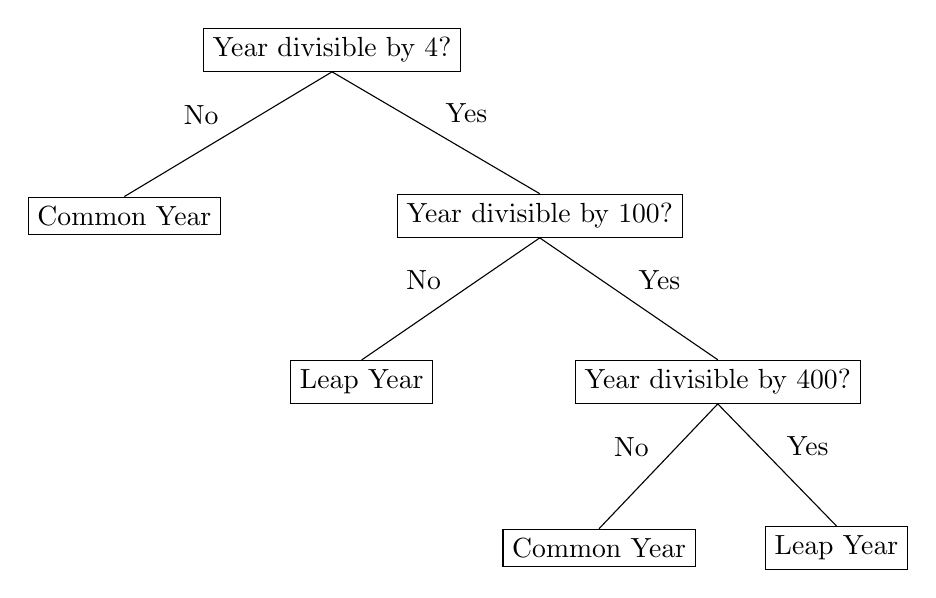
\begin{tikzpicture}[every tree node/.style={draw}]
        \tikzset{level distance=60pt, sibling distance=25pt}

        \Tree [.{Year divisible by 4?} 
                \edge node[auto=right] {No};
                [.{Common Year} ]
                \edge node[auto=left] {Yes};
                [.{Year divisible by 100?} 
                    \edge node[auto=right] {No};
                    [.{Leap Year} ]
                    \edge node[auto=left] {Yes};
                    [.{Year divisible by 400?} 
                        \edge node[auto=right] {No};
                        [.{Common Year} ] 
                        \edge node[auto=left] {Yes};
                        [.{Leap Year} ]
                    ] 
                ] 
            ] 
                
    \end{tikzpicture}

    \caption{A simple decision tree, determining if a year is a leap year.}\label{fig:decision_tree}
\end{figure}

Such a decision tree is shown in Figure~\ref{fig:decision_tree}. The input for 
this tree would be a set of year numbers. Taking one of these numbers, its 
properties (or features) can be used to answer the question posed by the root 
node. Following the appropriate edge, and answering any following questions will
finally lead to a leaf node. The leaf node reached will contain the 
classification of the input; the answer whether the year number is a leap year.

\subsubsection{Constructing Decision Trees}

In some cases, the construction of a decision tree may seem obvious; nodes can 
be constructed to clearly separate classes and the resulting classification is
free of error. But as the size of datasets and the amount and complexity of 
their features rise, a clearly defined way of constructing decision trees is 
required. To determine along what quality to split a dataset, that is, through
which question to determine the further progression through the tree, every
possible new node must be evaluated through a common measure. This measure 
determines, which split is chosen to achieve the best overall performance for
the classification tree. One such measure, the \textit{purity} of a split will
be utilized here.
Purity describes how well a node, or its question, manages to split the dataset
along its classes. If, after one node, no part of the input is lumped together
with one of a different class, that node is completely pure. Inversely, the more
mixed between classes the output of a node is, the more impure that node is.
Pure nodes are generally preferred, as they lead to smaller, more effective 
trees. Sorting by purity, nodes are connected starting at the root and branching
out into branches and leaves. The tree stops growing when either perfect purity
is achieved, i.e.~the entire set is correctly classified, no nodes are left or
a predetermined maximum tree depth is reached~\cite{classification_and_regression_trees,gini_index_vs_information_gain,decision_tree_learning}.

\subsubsection{\aclp{rf}}

A decision tree can in theory be used to classify any amount of data utilizing
a feature vector of arbitrary length. Should a tree not achieve full purity, 
there will always be an error in classification. Inversely, if a decision tree
achieves a perfect classification rate, this may mean it is overfitted on its 
training set. This means, as that model fits its training set, and only its 
training set, perfectly, it manages classification on any additional datasets
considerably worse than non-overfitted models. Additionally, individual trees
tend to be unstable; a change in a single node affects all of its children.
Slight changes in the dataset, such as random noise, can strongly affect the
construction and outcomes of a 
tree~\cite{elements_of_statistical_learning,classification_and_regression_trees}.

To avoid this, a collection of trees, sometimes called a forest, can be used. By
taking random samples of the training set per tree, selecting a small random subset of 
available features at each node and using the best (most \enquote{pure}) parameter to split on, a group of decision trees are constructed. When 
classifying a member of the test set, that member passes through every tree, 
generating a prediction from each. Using those individual classifications, the
member is then assigned to the class that received the most \enquote{votes}, 
i.e.~the most chosen class by individual trees. This ensemble of randomly 
generated trees forming a forest is known as a \acf{rf} classifier~\cite{random_forests_article,random_forests_web}. 

The accuracy of a tree are measured during its construction by splitting off a
portion of all available cases. This portion is then used to test already 
constructed trees. Additionally, this enables the determination of individual
features' contribution to the final result. First, the reserved set is classified
using the constructed forest, counting correct votes for each case. Then, a 
single variable is swapped randomly between cases and they are classified again.
If performance suffers after swapping the variable, this variable contributes
strongly to the forest's performance, making it more 
important~\cite{random_forests_article,random_forests_web}. 

\subsubsection{Evaluation}

\acp{rf}, as with classifier models in general, can be evaluated using a set of
metrics. The two methods explored here are the \textit{confusion matrix} and 
the \textit{\acf{roc} curve}, using hold-out evaluation. Note, that although the evaluation of a model 
does not by itself have any influence on the performance of a model, it has a
strong influence on the perceived performance of a model. Depending on 
evaluation method, a model can be perceived to perform better or 
worse~\cite{evaluating_learning_algorithms}. The methods treated here were 
chosen because of their relatively common use in similar studies~\cite{multisite_rectal_radiomics,radiomics_analysis_pcr_rectal}. % TODO: Does this need a citation?

In the context of this thesis, all metrics described are calculated based
on the process of hold-out evaluation. This involves splitting an available 
dataset into two parts; a \textit{training set} and a \textit{testing set}.
The training is used in conjunction with known class labels to construct a 
classifier. The class labels are used to estimate and minimize the expected 
error rate of that classifier. Then, the testing set is passed to the model,
stripped of labels. By measuring its performance in classifying the testing set,
a model is evaluated~\cite{evaluating_learning_algorithms,fundamentals_of_machine_learning}.

The confusion matrix contains information about every classification. For $n$ 
classes in the dataset it forms an $n \times n$ matrix. In this matrix, the sum 
of all entries in row $i$ represents the amount of cases assigned to class $i$ 
by the classifier. Meanwhile, the sum of elements in row $j$ represents the 
number of elements that class $j$ actually contains. Every cell $ij$ in the 
matrix represents how many cases of class $j$ have been predicted to belong to 
class $i$. If $i = j$, cell $ij$ contains \textit{true} predictions. 
If $i \neq j$, all predictions in that cell are \textit{false}~\cite{evaluating_learning_algorithms}.

For a binary classification, such as \enquote{\ac{pcr} of a patient}, 
classifications can be separated into four distinct groups. If a prediction 
accurately assigns a label ($i = j$), that prediction is true; is the prediction 
positive (\enquote{the patient will recover}),
it is \iac{tp}, if not (\enquote{the patient will not recover}), it is \iac{tn}. In contrast, if the prediction 
fails ($i \neq j$), a positive assignment results in \iac{fp} (\enquote{the patient was expected to recover, but did not}), while a negative
prediction yields \iac{fn} (\enquote{the patient recovered, but was not expected to do so}).
These relations between predicted and actual outcomes are shown in Table~\ref{tbl:confusion_matrix}.

\begin{table}[h]
    \centering
    \begin{tabularx}{12cm}{Y!{\vrule width 1.5pt}Y|Y}
         & \textbf{Positive Prediction} & \textbf{Negative Prediction} \\\noalign{\hrule height 1.5pt}
        \textbf{Positive Case}  & \textit{\acf{tp}} & \acf{fn} \\ \hline
        \textbf{Negative Case} & \acf{fp} & \textit{\acf{tn}} \\
    \end{tabularx}\caption{A confusion matrix for binary classification. The vertical axis going from top left to bottom right represents correct classifications, written in \textit{italics}. Adapted from~\cite{evaluating_learning_algorithms}.}\label{tbl:confusion_matrix}
\end{table}

The total number of predictions in one of these groups reveals little about the
performance of a classifier. A high total count of \ac{tp} classifications may 
just as well stem from a large sample size as from a well constructed model.
For this reason, a \textit{\ac{tpr}} can be calculated. By setting in 
contrast the number of \ac{tp} predictions to that of positive cases in the dataset, the probability of a positive case being recognized as such is found. This
ratio, as shown in Equation~\ref{eq:true_positive_rate}, can be applied to any
group; by dividing the number of true assignments to a class by that of the 
members of that class, the rate of recognition of that class is
gained. The same can be calculated from false assignments, yielding the rate of
misclassification~\cite{evaluating_learning_algorithms,fundamentals_of_machine_learning}.

\begin{equation}
    \text{\acl{tp} Rate} = \frac{\text{\acl{tp} Predictions}}{\text{Positive Cases}} = \frac{\acs{tp}}{\acs{tp} + \acs{fn}}
    \label{eq:true_positive_rate}
\end{equation}

In the context of classification, two more metrics based on the confusion matrix
are used; \textit{sensitivity}, which equates to the \ac{tpr}, and 
\textit{specificity}, which represents the ratio of \ac{tn} predictions to the 
sum of \ac{fp} and \ac{tn} predictions, also known as the \ac{tnr}. Respectively, these measures describe
which portion of actually positive and actually negative cases were recognized 
as such. A composite metric of these scores is the \textit{balanced accuracy}, 
defined as in Equation~\ref{eq:ba}~\cite{evaluating_learning_algorithms,fundamentals_of_machine_learning,balanced_accuracy_and_posterior}.
By combining information about both the recognition of positive and negative 
cases, it provides an overview of the model's total accuracy. This is especially
useful, if the dataset is unbalanced, i.e.~if one label is more abundant than 
the other. If a dataset consisted of \SI{90}{\percent} positive cases, and only
\SI{10}{\percent} negative cases, a model labelling every case as 
\enquote{positive} would achieve both a \enquote{normal} accuracy of 0.9 
and \iac{tpr} of 1.0. By giving \ac{tnr} an equal 
weight in the total score, the accuracy (now balanced) would sink to 0.5.

\begin{equation}
    \text{Balanced Accuracy} = \frac{\frac{\text{\acl{tp} Predictions}}{\text{Positive Cases}} + \frac{\text{\acl{tn} Predictions}}{\text{Negative Cases}}}{2} = \frac{\acs{tpr} + \acs{tnr}}{2}
    \label{eq:ba}
\end{equation}

Another metric for model performance can be constructed by seeking an ideal 
balance in the trade-off between the \ac{tpr} and the \ac{fpr}. This is 
possible, because \iac{rf} classifier does not solely put any case into one of two 
classes. Due to its assembly of voting trees, \iac{rf} classifier can return
the (estimated) probability of a case being positive. By moving the threshold
for the minimum probability to classify a case as \enquote{true}, the 
sensitivity of a model can be raised or lowered. If the model would accept all cases as 
true (a threshold of 0.0), it would achieve \iac{tpr} of 1.0, while
raising its \ac{fpr} to 1.0. As the \ac{fpr} is directly correlated to the 
\ac{tnr}, this being $\text{\ac{tnr}} = 1.0 - \text{\ac{fpr}}$, this significantly lowers the balanced accuracy. 
To achieve the best possible trade-off between these two metrics, \iac{roc} 
curve can be constructed, by plotting the \ac{tpr} against the \ac{fpr}. One such 
curve is shown in Figure~\ref{fig:roc}, representing the results of differing 
classifier thresholds.


% Adapted from https://tex.stackexchange.com/questions/464887/drawing-roc-curve-analysis
\newcommand{\roccolor}{purple}
\begin{figure}[H]
    \centering

    \begin{tikzpicture}
        \begin{axis}[
        title={\acl{roc} Curve},
        xlabel={\acl{fpr}},
        ylabel={\acl{tpr}}, 
        xmin=0.0, 
        xmax=1.0,
        ymin=0.0,
        ymax=1.0,
        ]

        % To shade between
        \path [name path=xaxis]
            (0,0.5) --
            (1,0.50) --
            (1,1);

        \addplot [name path=roc, \roccolor] coordinates {
            (0, 0)
            (0, 0.15)
            (0.1, 0.15)
            (0.1, 0.25)
            (0.2, 0.25)
            (0.2, 0.6)
            (0.3, 0.6)
            (0.3, 0.75)
            (0.5, 0.75)
            (0.5, 0.85)
            (0.8, 0.85)
            (0.8, 0.95)
            (0.95, 0.95)
            (0.95, 1)
            (1, 1)
        };

        % \addplot [
        % thick,
        % color=blue,
        % fill=blue, 
        % fill opacity=0.5
        % ]
        % fill between[
        %     of=roc and xaxis,
        %     soft clip={domain=0:1},
        % ];

        
        \addplot [red, dashed] coordinates {
            (0, 0)
            (1, 1)
        };


        \end{axis}
\end{tikzpicture}
\caption{The \ac{roc} curve of a fictional classifier. The solid \roccolor{} line shows the performance of the model, while the dashed red line shows the result of random guesses. The larger the area below the curve, i.e.~the farther the model is away from random guessing, the bigger the \acs{auc} and the performance of the model. A curve running below the center line would suggest swapped labels.}\label{fig:roc}
\end{figure}


The \ac{roc} curve shows the ability of a model to recognize a positive case as
such, against the probability of misidentifying a negative case as positive.
If these probabilities are equal, the model is guessing randomly. The total 
performance of the model at the full range of thresholds can be calculated by
the deviation from random guesses, i.e.~the center line. \Iac{roc} curve 
usually runs above this line, as the opposite would suggest swapped labels. 
Therefore, measuring all space below the curve yields a new metric, the 
so-called \acf{auc}~\cite{evaluating_learning_algorithms,fundamentals_of_machine_learning}.

%% !TEX program = xelatex

\section{Theory}

% \iffalse
% % !TEX program = xelatex

\section{Data preparation}
% TODO: What was the correct term for this?

\iffalse{}
\subsection{Normalization}
\fi

\subsection{3D and 2D Annotations}

% TODO: "mention first how were 2D annotations created. Why only 2D? -> trade-off time consumption vs. value"
% TODO: Why this approach for 3D-reconstruction?
% Inital thoughts: 
%  - Most current algorithms are ML-based.
%  - Some require medical knowledge
%  - Too few 3D annotations to check/train ML model
%  - Is it a good idea to base ML model on another ML model?
% Read "auto_vs_semiauto_vs_manual_anno.pdf" when not half asleep. Even "automatic" seems
% to require human intervention(?).
% ~prostate_automatic_annotation.pdf seems to suggest ellipsoid a-priori shape for tumors.~
% Misunderstanding: shape of prostate (not tumor!) was described

While all \ac{mri} scans in the dataset consist of 3-dimensional data, 
most are segmented along only 2 axes, forming a flat slice in the scan.
An example would be an annotation that cover only the sagittal plane. 
Note, that the annotation file for 
a 2-dimensional annotations is still a 3-dimensional image, but the 
\ac{roi} is marked only in one slice, as can be seen in Figure~\ref{fig:2dvs3d}.

\begin{figure}[H]
    \centering
    \includegraphics[width=1.0\textwidth]{img/mo0501229884a_marked.png}
    \caption{A manual tumor annotation. A 2-dimensional annotation is marked in red. As it is formed by voxels, it still possesses a non-zero width. If combined with the annotation marked in green, it forms a 3-dimensional annotation. From right to left: axial plane, sagittal plane and coronal plane.}\label{fig:2dvs3d}
\end{figure}

For ease of understanding, 
2-dimensional annotations will be treated as 2-dimensional images, if not
noted otherwise.
This mixture of annotation types poses a set of problems; requirements of radiomics
features and consistency. A group of PyRadiomics' features, namely 
\enquote{Shape Features (3D)} rely on a 3-dimensional \ac{roi}. With a largely 2-dimensional
dataset, these features would need to be excluded. Furthermore, it has been suggested, 
that analysis of complete tumors may be more representative
of a tumor's features than analysis of its biggest slice, especially in colorectal 
tumors~\cite{whole_tumor_vs_cross_section}\cite{rad_in_prec_med}.
In contrast, some scans in the dataset are annotated along 3 dimensions. 
This inconsistency in input data may lead to varying ratios of 2D and 3D 
annotated data in subsamples, strongly impacting reproducibility.

\subsubsection{Creation of 2D annotations.}
% Describe 2D-ification
As all 3D annotations in the dataset were created manually, they can neither
be recreated automatically nor reliably, without involving the original annotators.
To avoid a mix of manual and automated 3D annotations, the same 3D reconstruction 
algorithm will be applied to all annotations.
Manual 3D annotations will therefore treated as 2D annotations 
and must be reduced by one axis.

To lose as little information as possible, while still dropping information along the third
axis, the largest area along two axes in the 3D annotation is used. To determine this slice
of the original annotation, the annotation is split into 2-dimensional slices along each axis.
For each slice, all marked voxels marked as part of the \ac{roi} can be counted. As the axes of 
these voxels may be unevenly scaled, the voxel count must be multiplied with a correction factor to account for
the different axis scales. The largest area after application of the correction factor is the 
largest 2D-slice by area, and therefore the new 2D annotation.

\subsubsection{Creation of 3D annotations.}
% Describe inverse distance transform + optimization steps
% Now, the fully 2D-annotated dataset can be converted to 3D annotations.
Now, 3D annotations can be reconstructed from the fully 2D annotated dataset.
The algorithm used here was chosen to be simple to implement and reproduce.
It is based on \enquote{inverting} a 2-dimensional euclidean distance 
transformation. % Don't forget to include the figure


The distance transform assigns each pixel in an image a value based on the
pixel's distance to the nearest pixel with a non-zero color 
value~\cite{2020SciPy-NMeth}. Here, the distance is determined by the 
L\textsubscript{2} norm, adjusted for potentially uneven scaled axes. As 
demonstrated in Figure~\ref{fig:2d-annotation} using this transformation on a 
2-dimensional annotation yields the distance of each pixel inside the 
\ac{roi} to the nearest pixel outside the \ac{roi}. This property will 
henceforth simply be referred to as a pixel's \enquote{2D distance}.

\begin{figure}[H]
    \centering
    \begin{subfigure}[t]{0.4\textwidth}
        \includegraphics[width=\textwidth]{img/img_base_mr1a.jpg}
        \caption{Base image. White areas mark the \ac{roi}.}\label{fig:2d-base}
    \end{subfigure}
    ~
    \begin{subfigure}[t]{0.4\textwidth}
        \includegraphics[width=\textwidth]{img/img_dist_mr1a.jpg}
        \caption{Euclidean distance transform implemented by~\cite{2020SciPy-NMeth}. Lighter colors indicate a greater distance.}\label{fig:2d-dist}
    \end{subfigure}
    \caption{A 2-dimensional \ac{roi} annotation. The contrast of both images has been increased to allow for easier viewing.}
    \label{fig:2d-annotation}
\end{figure}

% Draft 1
% To create a 3-dimensional annotation, new layers of pixels along the new
% third axis will be added. If any new pixel is closer to a pixel that is 
% part of the original \ac{roi} than the original pixel's 2D distance (as 
% determined by the distance transformation), the new pixel is also made part
% of the \ac{roi}.

% Draft 2
To create a 3-dimensional annotation, new layers of voxels along the new
third axis will be added. The distance of each new voxel in relation to 
every pixel in the original \ac{roi} is determined. Should the 
\enquote{2D distance} of a pixel in the \ac{roi} be larger than the 
distance between that pixel and the new voxel, the new voxel is added to 
the new \ac{roi}. A pseudo-code implementation of this algorithm is shown
in Listing~\ref{code:3dpseudo}.

\begin{lstlisting}[caption=3D reconstruction., label={code:3dpseudo}]
    annotation_2d = get_largest_slice(annotation_original)
    annotation_2d_distances = euclidean_distance(annotation_2d)

    for voxel_new in annotation_new:
        for pixel_old in annotation_2d:
            if euclidean_distance(voxel_new, pixel_old) <= annotation_2d_distances[pixel_old]:
                annotation_new[voxel_new] = 1
                break

\end{lstlisting}

This leads to a new 3-dimensional annotation, symmetrical along the initial
2-dimensional annotation slice. As can be seen in Figure~\ref{fig:3d-annotation},
the thickness of the annotation increases with the \enquote{2D distance} of 
the underlying pixels. Should the 2-dimensional annotation along the base 
layer be circular, the 3-dimensional annotation will approach a sphere.



% Describe check for new pixels (is this pixel along the 3rd axis closer
% than roi pixel's distance? -> Include in roi.)


\begin{figure}[H]
    \centering
    \begin{subfigure}[t]{0.4\textwidth}
        \includegraphics[width=\textwidth]{img/3d_mr1a.png}
        \caption{A 3-dimensional plot of the annotation. Note the uneven resolutions along different axes.}\label{fig:3d-3d}
    \end{subfigure}
    ~
    \begin{subfigure}[t]{0.4\textwidth}
        \includegraphics[width=\textwidth]{img/heatmap_mr1a.png}
        \caption{The 3-dimensional annotation projected back onto the original 2-dimensional annotation. The shape is symmetrical along the 2-dimensional base layer.}\label{fig:3d-2d}
    \end{subfigure}
    \caption{The 3-dimensional annotation generated from a 2-dimensional annotation. Both plots are cropped to the \ac{roi}.}\label{fig:3d-annotation}
\end{figure}

\subsubsection{Optimization of 3D-reconstruction}

The algorithm described above is inefficient for large images. 
Its complexity can be described by $\mathcal{O}(n~\cdot~m)$, where $n$ is the 
total number of voxels in the new annotation and $m$ is the number 
of voxels (or pixels, as it only uses two axes) in the original 2-dimensional
annotation. As tumors (and therefore tumor annotations) cover only small 
parts of the total 3D image, most pixels in the new annotation ($n$) are 
checked\footnote{\enquote{Checked} refers a voxel's distance to a pixel 
in the original annotation being calculated and compared to that pixel's 
\enquote{2D-distance}.} for no reason; the distance of the majority of 
voxels to the \ac{roi} is far greater than the \enquote{2D-distance} 
of any pixels in the original annotation.

The following changes in the algorithm defined earlier aim to reduce the
amount of unnecessary distance measurements. Instead of checking every
new voxel in the new annotation for its distance to a pixel in the original
annotation, a cube of influence is calculated for that pixel. In the center
of this cube of influence lies a pixel in the original annotation. The 
size of the cube is determined by the pixel's \enquote{2D-distance}; 
the \enquote{2D-distance} is divided by each axis' scale. This, rounded down
to the next whole number, gives the \enquote{radius} of the cube along
each axis. For example, a pixel may possess a \enquote{2D-distance} of
10 mm. For axis scales of 3 mm, 3 mm and 12 mm, the cube of influence would
measure 7$\times$ 7$\times$ 1 voxels. These dimensions result from the 
radii (3, 3, 0) being applied in both directions (e.g. \enquote{forward} 
and \enquote{backward}) and the initial voxel being added in the center. 
Each voxel in this cube is now checked to be closer to the original pixel
than the pixel's \enquote{2D-distance}. If so, the voxel is added to the 
new annotation. Should the voxel already be part of the new annotation 
(because it was already assigned this value through comparison to an
earlier pixel), it is not checked again.

\subsubsection{Rationalization}

As of time of writing, the (semi-)automatic segmentation of tumors is 
a problem without a generally agreed-on solution. Current approaches include
\ac{dl} based approaches such as~\cite{u-net_auto_anno} and~\cite{dl_rectal_segmentation}. 
To train \ac{dl} models accurately, a certain amount of input data is required, both as ground
truth and training data. In~\cite{u-net_auto_anno}, 300 3-dimensionally annotated \ac{mri} scans
are used for training, validation and testing, while~\cite{dl_rectal_segmentation} uses
a total of 140 scans. These quantities of scans far outweigh the total count of 5 3-dimensionally 
annotated scans available here.

Another common approach is semi-automatic segmentation. \cite{auto_and_semiauto} proposes 
both an automatic and a semi-automatic method of segmentation. While lightening the burden on
medical professionals, both of these methods rely on prior medical knowledge, or at the 
very least, human interaction. As the relevant medical information is not available in
this project, no approach described by~\cite{auto_and_semiauto} can be utilized.
Different semi-automatic segmentation methods, even if they may not depend on any medical
training, are still, by definition, based on human interaction. As one the main goals
of the 3D-reconstruction described here is to be easily reproducible, introducing a 
human factor may be detrimental this objective.

% Semiauto - not feasable due to missing medical knowledge.
% Therefore going for a "good-enough" method. Reference both automatic and semi-automatic methods of "Automated and Semiautomated Segmentation of Rectal Tumor Volumes on Diffusion-Weighted MRI: Can It Replace Manual Volumetry?" as both require human intervention
% 3D tumors seems to be round-ish. Maybe look for more data confirming or confute this.

% Optimization: Could you just cut down (empty) new annotation to size
% of old annotation (make square of 2D to cube)
% Implement ^this, benchmark both, use faster. Describe benchmark in paper
% NVM, ^this is still O(n*m), while per-pixel cube approach still skips
% most n pixels

% Maybe count distance measures in original and optimized method and 
% plot both?

% For results/improvement: Describe why balanced accuracy and not overall accuracy
% is important for unbalanced dataset

\section{Machine Learning Model}

As mentioned earlier, the main goal of this work is to, with reasonable 
accuracy, predict the \ac{pcr} of a patient. Essentially, this creates a 
question of \enquote{Yes} or \enquote{No}. A process assigning its input data to 
one of two categories can be represented as a two-class classifier. 

The classifier chosen here is the \enquote{Random Forests} model. If offers 


\subsection{Implementation}

\texttt{sklearn} offers an implementation of a random forest classifier through
its \\\texttt{sklearn.ensemble.RandomForestClassifier} class. This implementation
was chosen for a host of reasons. Being written in Python, it offers a 
accessible and easy to use interface and compatibility with other feature-rich
data analysis tools (such as, but not limited to, \texttt{numpy}, 
\texttt{pandas} and \texttt{matplotlib}). Additionally, being an open-source
project, the library is both cheap (i.e.~free) to acquire and use 
(assuming no license violations) and easy to version and distribute, increasing 
reproducibility. 



\subsection{Model Selection}
% Why random forest and why in sklearn?

\subsection{Training}
% Sample functions and parameters

\subsection{Feature Filtering}

With an input vector of 1743 features, it is not expected that each feature 
affects the final classification decision equally, or at all. 
A list of the \enquote{importance} of each feature, i.e.~the impact its value 
will have on that final decision, can be generated after a random forest is 
built.

From this list of importances we can see, that a significant portion of our 
input data has very little importance in our model. Although not helpful for our 
purpose, these features still must be considered in building our random forest 
and may be chosen to form decision trees, introducing additional but ultimately 
pointless nodes into our decision trees. This may negatively impact the 
performance of the model~\cite{elements_of_statistical_learning}.
For this reason, features of low importance will be filtered out.

\subsubsection{Determining Importance}

The choice of training and testing inputs determine the resulting model, the 
importance of individual features and its (balanced\footnote{Unless explicitly
stated otherwise, all mentions of \enquote{accuracy} refer to \enquote{balanced
accuracy}.}) accuracy. As the input sets are split randomly, both the accuracy
of the model and features' contributions to the result may vary strongly.

To avoid basing the decision about a feature's relevancy to the overall result
by a single model, which may represent an outlier, the importance is determined
by a weighted average over multiple models. To reduce the impact inaccurate 
models on the total priority of features, each model is weighted by its 
accuracy, adjusted to conform to a range of \enquote{0} to \enquote{1}, for 
the worst and best possible result respectively. Assuming the importance of 
a feature is calculated over \(m = 100\) models, where \( b_n \) is the 
(adjusted) accuracy of model \(n\) and \(i_n\) is the importance of this 
specific feature in this specific model, the weighing can be described as in
Equation~\ref{eq:weighted_average}.

\begin{equation} \label{eq:weighted_average}
    \sum_{i=1}^{m} \frac{b_n \cdot i_n}{m}
\end{equation}

When applied to all available features, the resulting importance distribution
can be seen in Figure~\ref{fig:importance_dist}. Note the peak at, or near, 
zero.

\begin{figure}[H]
    \centering
    \includegraphics[width=\textwidth]{img/feature_importance_dist.png}
    \caption{Amount of fe.}\label{fig:importance_dist}
\end{figure}

\subsubsection{Filter Levels}

With a set of weighted importances, a filter can be created. This filter drops
all features with an importance below a certain level. A filter has been applied
for a 100 equally distributed levels between \enquote{0} and the maximum 
importance in the list of weighted importances. For each of these filters, the
average over a 100 models has been calculated, the results of which can be seen
in Figure~\ref{fig:importance_filter}.

\begin{figure}[H]
    \centering
    \includegraphics[width=\textwidth]{img/filter_levels_accuracy_logcount.png}
    \caption{Amount of feature per model, accuracy and variance of accuracy of 
    this model over the filter level. Note the logarithmic y-axis for Feature Count.}\label{fig:importance_filter}
\end{figure}

Without filtering, the accuracy of the model sits at a base level of 
0.6359. Removing zero to very low importance features initially barely improves
accuracy. 
% Improvements to ~0.66 start at 0.000251708540042472 with 1057 features. Note, this is the flawed run, correct his after new run.
% TODO: Analyze the results further

\subsection{Evaluation}
% Not exactly sure yet.
% If applicable, show process of selecting important radiomics features

\section{Results}
% Hopefully, one day

\section{Discussion}
% Optionally, if there's something interesting to say about the results. 
% Maybe compare to similar paper.
% \fi
\newpage{}
\section{Materials and Methods}

% Add small intro here 
This section gives an overview about the dataset used for classification, as 
well as a conceptual overview of the experimental setup and the assumptions 
behind that setup. For a source-code 
focused view of the project, refer to Section~\ref{sec:implementation}.

\subsection{Dataset}\label{sec:materials_dataset}

Though this thesis treats the analysis of a set of \ac{mri} scans, these scans
were not produced by the author. The dataset was provided % TODO:
by the Institute of Radiology % TODO: Don't forget new scans
of the \ac{salk}. It consists of \ac{mri} scans of 102 patients, where 24 reached 
\ac{pcr}. Due to mismatches in geometry between annotation and scan, 9 scans
could not be used. This leaves 93 patients, 22, or \SI{23.366}{\percent}, of which achieved 
\ac{pcr}. All scans were manually annotated.

The dataset may not be published, as it underlies an obligation of anonymity to 
the patients the scans were recorded of. Additional available metadata to that 
mentioned above is listed in the appendix under Section~\ref{sec:mri_metadata}.

The exact definition of \ac{pcr} is not always clear or consistent.
In this context, it signifies absence of cancer tissue
around the site of occurrence after treatment. This includes \enquote{[\dots] 
the total absence of neoplastic cells [tumors] in the rectal wall, mesorectum, 
and mesorectal lymph nodes}~\cite[p.~2823]{Zorcolo2012}\cite{clinical_and_oncological_results_of_pcr}.
% TODO: Describe metadata, maybe add table in appendix?
% TODO: Who annotated the dataset - Kinda done

The dataset is not annotated consistently; most scans contain a 2-dimensional 
annotation, marking a slice of tumor, while \threeDcount{} scans are annotated along all 
three axes. To avoid inconsistencies, all annotations were interpolated to form
a 3-dimensional annotation from their largest slice, as described 
in~\ref{sec:3d_and_2d}.

\subsection{Choice of Tools}

As is popular with machine learning projects, this program is implemented in 
Python\footnote{\hyperlink{https://www.python.org/}{More information available 
at https://www.python.org/}.}. It offers the possibility of quick prototyping, 
intuitive and easily readable syntax and, most importantly, a large tool set for
both radiomics and machine learning applications. 

To address the earlier mentioned problem with the definition and extraction of
radiomics features, a widely available and well documented library was chosen.
PyRadiomics\footnote{More information available at 
\hyperlink{https://www.radiomics.io/pyradiomics.html}
{https://www.radiomics.io/pyradiomics.html}.\\Documentation available at 
\hyperlink{https://pyradiomics.readthedocs.io/en/latest/}
{https://pyradiomics.readthedocs.io/en/latest/}.} covers, and is compatible to,
most features defined by the \ac{ibsi}, while documenting any differences in 
features definition or calculation (such as correcting for negative values, 
which may not be covered in the \ac{ibsi} formula).
Additionally, PyRadiomics offers tools to pre-process data, e.g.~normalization
of input images or passing input images through predetermined filters.

Next, the features extracted by PyRadiomics have to be processed. In the context
of this project, this means to classify an input image into two categories: 
expected \enquote{\ac{pcr}} or \enquote{non-\ac{pcr}}. As discussed earlier, % TODO: make sure to discuss this earlier
a random forest classifier was chosen for this task. The toolkit used to 
implement this classification model is \texttt{sklearn}, which offers an 
implementation of a random forest classifier through
its \\\texttt{sklearn.ensemble.RandomForestClassifier} class. It offers an
accessible and easy to use interface and compatibility with other feature-rich
data analysis tools (such as, but not limited to, \texttt{numpy}, 
\texttt{pandas} and \texttt{matplotlib}). Additionally, being an open-source
project, the library is both cheap (i.e.~free) to acquire and use 
(assuming no license violations) and easy to version and distribute, increasing 
reproducibility. 

As a connection between extraction and classification and analysis of results, a
multitude of other libraries are required. Though important in their own rights,
these libraries are not of special interest in the context of this thesis and 
will be addressed when relevant, instead of introducing them here.

\subsection{Experimental Setup}\label{sec:experimental_setup}

% Short summary of what I do

As stated earlier, this thesis aims to determine, if \ac{pcr} of a colorectal
tumor patient can be predicted through a radiomics-based classification model,
using \ac{mri} scans as input. To be considered successful, the model has 
to achieve a (balanced\footnote{Unless explicitly
stated otherwise, all mentions of \enquote{accuracy} refer to \enquote{balanced
accuracy}.}) accuracy deviating significantly from 0.5, or \SI{50}{\percent}. 

The model chosen is \iac{rf} classifier. The model is trained on a set composed
of \SI{70}{\percent} of all \ac{pcr} patients and an equal amount of non-\ac{pcr} patients,
both chosen randomly. The testing set consists of all remaining patients.
Each patient is represented by \iac{mri} scan accompanied by an annotation 
marking the contained tumor. Before feature extraction, this annotation is 
passed through a common extrapolation algorithm to create a 3-dimensional 
\ac{roi}. From this, radiomics features are extracted using PyRadiomics. A 
common extractor is used for all patients; its configuration file can be found
in the appendix under Listing~\ref{code:pyrad_config}. The majority of available
features are extracted, as a large fraction will be filtered out later.

Using these features, \ac{rf} classification models are constructed. Each model
is composed of 1000 estimators, each fully grown~\cite{sklearn_docs}. The 
performance for each model is evaluated over 100 instances of that model.
These 100 models share their configuration, but are trained and tested using 
differently split datasets and receive different random-states.

With these classification models, two groups are determined; features that have
a favorable impact on the accuracy of the model and feature groupings that may
improve accuracy in combination. First, features are sorted by their 
contribution to a set of \enquote{sacrificial} models processing all available features.
Then, features below a certain significance are dropped, to determine the 
optimal level of minimal importance. The remaining features are considered 
significant to the success of the classification model. If the model fed with
the \enquote{ideal} set of features reliably performs better than random chance,
the experiment is considered successful.

To determine possible synergies between features, models based on related 
features are constructed. Relation is considered in three categories; source image,
feature group and feature extraction method. If a model based on a grouping performs better
than the earlier \enquote{sacrificial} model, % TODO: Check the next part
its performance is compared to the average \enquote{importance} of features making up
that grouping. If the performance of that grouping is better than the 
expected performance for its average \enquote{importance}, the grouping is 
considered \enquote{synergetic}.

\subsection{Hypothesis}\label{sec:hypothesis}

A significant correlation between features extracted from annotated \ac{mri} 
scans and patient \ac{pcr} is expected. This is based on the results of earlier 
studies (compare Section~\ref{sec:state_of_research}) investigating this relationship 
through comparable means. 

As for accuracy, the filtering of less \enquote{helpful} features is expected to
improve the final result. Especially the removal of zero-importance features 
should significantly improve performance through the removal of statistical
\enquote{noise}~\cite{elements_of_statistical_learning}. Whereas the removal 
of low-importance features is expected to have a positive impact, the existence 
and detection of \enquote{synergetic} features is though to be possible, but not
certain. 

\newpage{}
\section{Implementation}\label{sec:implementation}

This section covers the details of implementing a program spanning the workflow
of a machine learning model based on features extracted through a radiomics 
library. Overall, this can be roughly sectioned into three conceptual stages; 
preparation of the dataset, extraction of features and training and evaluation 
of the classifier model.


% Overview here

\subsection{Code Structure}\label{sec:code_structure} % Temporary title

To represent the dataset, a class exists representing one single patient. This 
class, \texttt{TestCase}, consists of \iac{mri} scan, the corresponding 
annotation, the \ac{pcr} status of the patient and the metadata associated with 
the scan. On instantiation, the existence of both 
input images is checked, along with save-files from previous executions. These
files preserve information from prior executions, enabling computationally 
intense tasks to be skipped, if related settings have not been changed. If a 
related save-file exists, information is restored from that file; if not, the 
file is created after the information becomes available. Save-files are 
identified in a way that aims to preserve the context they were created in; this 
method and its benefits and issues are treated in Section~\ref{sec:save_management}.
The metadata these files, and in turn the class itself, consists of two sets of data.

Firstly, a second annotation. This second annotation is generated from the 
original annotation through an algorithm described in more detail in 
Section~\ref{sec:3d_and_2d}. This algorithm, applied consistently to every 
original annotation is an attempt to even out inconsistencies in the original 
dataset through a simple, easily reproduced method.

Lastly, the radiomics feature vector. This contains a list of feature 
identifiers and their respective value. The identifier unambiguously assigns 
each feature to the source image it was extracted from (or, the filter that was 
applied to that image), the feature group it belongs to and the features 
individual name (a textual representation of the feature extraction method). An overview about filters and feature groups is given in 
Section~\ref{sec:radiomics_features}, whereas more detail is given in~\cite{py_rad_docs}.

% Explain process in overview. If detail is needed, reference dedicated section.
% For example: "If the annotation exists, a 3-dimensional annotation will be 
% interpolated. For a in-depth look at this extrapolation, refer to \ref{sec:3d_and_2d}."
%
% Or something like that

The dataset consists of more than one patient. Additionally, to fulfill their 
full function, each instance of a patient's representation depends on shared 
resources, such as the feature extractor's configuration. To manage the entirety
of test cases and keep common data synchronized between them, the 
\texttt{TestCaseCollection} class is utilized. 

The main focus of this class is to provide access to consistent sub-samples of 
the total dataset and to collections of their feature vectors.  As such, it 
manages the central feature extractor shared between \texttt{TestCase}s. This 
enables it to create random splits in the dataset, as described in 
Section~\ref{sec:sampling}, and return their combined feature vectors in a 
format parsable by \texttt{sklearn}'s classifier classes.

Now that the dataset can be split into multiple sub-sets, which provide input 
data for a classifier, such a model can be created. The connection between this
input data and the model is offered by the \texttt{ClassificationRun} class. 
It accepts a \texttt{TestCaseCollection}, information about desired sample 
ratios (see Section~\ref{sec:sampling}) and a filter, which selects the features
actually used for training the model specific to this execution (see 
Section~\ref{sec:feature_filtering}). After creating and training its 
classifier, \texttt{ClassificationRun} then stores the model's evaluation, 
i.e.~the testing data, along with generated predictions and their statistical 
descriptors, such as balanced accuracy. 

Although this evaluation data is already valuable on its own, it focuses only
on a single split of the total dataset, and on a single classifier model. 
Depending on which instance of a \texttt{ClassificationRun} is chosen, this could
artificially make the model seem better or worse than what would be 
representative by accidentally (or intentionally) \enquote{cherry-picking}
results. For this reason, a model is evaluated by calculating its accuracy as a
mean over multiple executions, each featuring a different training and testing 
set, along with a different Random Forest makeup, determined by differing 
random generator seeds. As such, each grouping of \texttt{ClassificationRun}s
is managed by a \texttt{ClassificationRunCollection}.

A \texttt{ClassificationRunCollection} is representative of one 
\enquote{experimental setup}; if the effect of differing hyperparameters or 
different feature filters should be compared, it is done using this class. 
Like the \texttt{ClassificationRun} instances it contains, it offers information
about the setup's performance. Similar to the \texttt{TestCaseCollection} class,
it keeps shared data consistent, such as dataset splitting information and 
feature filters. It also accepts a seed parameter for passing down to 
\texttt{ClassificationRun} instances. A collection of these instances is only
useful, as either their seed or parameters differ. As parameters are explicitly
being kept consistent between \texttt{ClassificationRun} instances, the seed
received from the overarching \texttt{ClassificationRunCollection} is counted up
from its base value for each new \texttt{ClassificationRun} instance. This 
ensures different, but reproducible, random-states.

Now with all classifications done, information each instance is preserved. 
Metrics such as \ac{roc} curve, targets (actual case labels) and predictions 
are saved to then be used to evaluate the model. This enables later analyzation
by additional metrics and their visualization, without the need to repeat the 
classification with the same parameters.

\subsection{Annotation Extrapolation}\label{sec:3d_and_2d}

% TODO: "mention first how were 2D annotations created. Why only 2D? -> trade-off time consumption vs. value"
% TODO: Why this approach for 3D-reconstruction?
% Initial thoughts: 
%  - Most current algorithms are ML-based.
%  - Some require medical knowledge
%  - Too few 3D annotations to check/train ML model
%  - Is it a good idea to base ML model on another ML model?
% Read "auto_vs_semiauto_vs_manual_anno.pdf" when not half asleep. Even "automatic" seems
% to require human intervention(?).
% ~prostate_automatic_annotation.pdf seems to suggest ellipsoid a-priori shape for tumors.~
% Misunderstanding: shape of prostate (not tumor!) was described

While all \ac{mri} scans in the dataset consist of 3-dimensional data, 
most are segmented along only 2 axes, forming a flat slice in the scan.
An example would be an annotation that cover only the sagittal plane. 
Note, that the annotation file for 
a 2-dimensional annotations is still a 3-dimensional image, but the 
\ac{roi} is marked only in one slice, as can be seen in Figure~\ref{fig:2dvs3d}.

\begin{figure}[H]
    \centering
    \includegraphics[width=1.0\textwidth]{img/mo0501229884a_marked.png}
    \caption{A manual tumor annotation. A 2-dimensional annotation is marked in red. As it is formed by voxels, it still possesses a non-zero width. If combined with the annotation marked in green, it forms a 3-dimensional annotation. From right to left: axial plane, sagittal plane and coronal plane.}\label{fig:2dvs3d}
\end{figure}

For ease of understanding, 
2-dimensional annotations will be treated as 2-dimensional images, if not
noted otherwise.
This mixture of annotation types poses a set of problems; requirements of radiomics
features and consistency. A group of PyRadiomics' features, namely 
\enquote{Shape Features (3D)} rely on a 3-dimensional \ac{roi}. With a largely 2-dimensional
dataset, these features would need to be excluded. Furthermore, it has been suggested, 
that analysis of complete tumors may be more representative
of a tumor's features than analysis of its biggest slice, especially in colorectal 
tumors~\cite{whole_tumor_vs_cross_section,rad_in_prec_med}.
In contrast, some scans in the dataset are annotated along 3 dimensions. 
This inconsistency in input data may lead to varying ratios of 2D and 3D 
annotated data in subsamples, strongly impacting reproducibility.

\subsubsection{Creation of 2D annotations}
% Describe 2D-ification
As all 3D annotations in the dataset were created manually, they can neither
be recreated automatically nor reliably, without involving the original annotators.
To avoid a mix of manual and automated 3D annotations, the same 3D reconstruction 
algorithm will be applied to all annotations.
Manual 3D annotations will therefore be treated as 2D annotations 
and must be reduced by one axis.

To lose as little information as possible, while still dropping information along the third
axis, the largest area along two axes in the 3D annotation is used. To determine this slice
of the original annotation, the annotation is split into 2-dimensional slices along each axis.
For each slice, all marked voxels marked as part of the \ac{roi} can be counted. As the axes of 
these voxels may be unevenly scaled, the voxel count must be multiplied with a correction factor to account for
the different axis scales. The largest area after application of the correction factor is the 
largest 2D-slice by area, and therefore the new 2D annotation.

\subsubsection{Creation of 3D annotations}
% Describe inverse distance transform + optimization steps
% Now, the fully 2D-annotated dataset can be converted to 3D annotations.
Now, 3D annotations can be reconstructed from the fully 2D annotated dataset.
The algorithm used here was chosen to be simple to implement and reproduce.
It is based on \enquote{inverting} a 2-dimensional euclidean distance 
transformation. % Don't forget to include the figure


The distance transform assigns each pixel in an image a value based on the
pixel's distance to the nearest pixel with a non-zero color 
value~\cite{2020SciPy-NMeth}. Here, the distance is determined by the 
L\textsubscript{2} norm, adjusted for potentially uneven scaled axes. As 
demonstrated in Figure~\ref{fig:2d-annotation} using this transformation on a 
2-dimensional annotation yields the distance of each pixel inside the 
\ac{roi} to the nearest pixel outside the \ac{roi}. This property will 
henceforth simply be referred to as a pixel's \enquote{2D distance}.

\begin{figure}[H]
    \centering
    \begin{subfigure}[t]{0.4\textwidth}
        \includegraphics[width=\textwidth]{img/img_base_mr1a.jpg}
        \caption{Base image. White areas mark the \ac{roi}.}\label{fig:2d-base}
    \end{subfigure}
    ~
    \begin{subfigure}[t]{0.4\textwidth}
        \includegraphics[width=\textwidth]{img/img_dist_mr1a.jpg}
        \caption{Euclidean distance transform implemented by~\cite{2020SciPy-NMeth}. Lighter colors indicate a greater distance.}\label{fig:2d-dist}
    \end{subfigure}
    \caption{A 2-dimensional \ac{roi} annotation. The contrast of both images has been increased to allow for easier viewing.}\label{fig:2d-annotation}
\end{figure}

% Draft 1
% To create a 3-dimensional annotation, new layers of pixels along the new
% third axis will be added. If any new pixel is closer to a pixel that is 
% part of the original \ac{roi} than the original pixel's 2D distance (as 
% determined by the distance transformation), the new pixel is also made part
% of the \ac{roi}.

% Draft 2
To create a 3-dimensional annotation, new layers of voxels along the new
third axis will be added. The distance of each new voxel in relation to 
every pixel in the original \ac{roi} is determined. Should the 
\enquote{2D distance} of a pixel in the \ac{roi} be larger than the 
distance between that pixel and the new voxel, the new voxel is added to 
the new \ac{roi}. A pseudo-code implementation of this algorithm is shown
in Listing~\ref{code:3dpseudo}.

\begin{lstlisting}[caption=3D reconstruction., label={code:3dpseudo}]
    annotation_2d = get_largest_slice(annotation_original)
    annotation_2d_distances = euclidean_distance(annotation_2d)

    for voxel_new in annotation_new:
        for pixel_old in annotation_2d:
            if euclidean_distance(voxel_new, pixel_old) <= annotation_2d_distances[pixel_old]:
                annotation_new[voxel_new] = 1
                break

\end{lstlisting}

This leads to a new 3-dimensional annotation, symmetrical along the initial
2-dimensional annotation slice. As can be seen in Figure~\ref{fig:3d-annotation},
the thickness of the annotation increases with the \enquote{2D distance} of 
the underlying pixels. Should the 2-dimensional annotation along the base 
layer be circular, the 3-dimensional annotation will approach a sphere.



% Describe check for new pixels (is this pixel along the 3rd axis closer
% than roi pixel's distance? -> Include in roi.)


\begin{figure}[H]
    \centering
    \begin{subfigure}[t]{0.4\textwidth}
        \includegraphics[width=\textwidth]{img/3d_mr1a.png}
        \caption{A 3-dimensional plot of the annotation. Note the uneven resolutions along different axes.}\label{fig:3d-3d}
    \end{subfigure}
    ~
    \begin{subfigure}[t]{0.4\textwidth}
        \includegraphics[width=\textwidth]{img/heatmap_mr1a.png}
        \caption{The 3-dimensional annotation projected back onto the original 2-dimensional annotation. The shape is symmetrical along the 2-dimensional base layer.}\label{fig:3d-2d}
    \end{subfigure}
    \caption{The 3-dimensional annotation generated from a 2-dimensional annotation. Both plots are cropped to the \ac{roi}.}\label{fig:3d-annotation}
\end{figure}

\subsubsection{Optimization of 3D-reconstruction}

The algorithm described above is inefficient for large images. 
Its complexity can be described by $\mathcal{O}(n~\cdot~m)$, where $n$ is the 
total number of voxels in the new annotation and $m$ is the number 
of voxels (or pixels, as it only uses two axes) in the original 2-dimensional
annotation. As tumors (and therefore tumor annotations) cover only small 
parts of the total 3D image, most pixels in the new annotation ($n$) are 
checked\footnote{\enquote{Checked} refers a voxel's distance to a pixel 
in the original annotation being calculated and compared to that pixel's 
\enquote{2D-distance}.} for no reason; the distance of the majority of 
voxels to the \ac{roi} is far greater than the \enquote{2D-distance} 
of any pixels in the original annotation.

The following changes in the algorithm defined earlier aim to reduce the
amount of unnecessary distance measurements. Instead of checking every
new voxel in the new annotation for its distance to a pixel in the original
annotation, a cube of influence is calculated for that pixel. In the center
of this cube of influence lies a pixel in the original annotation. The 
size of the cube is determined by the pixel's \enquote{2D-distance}; 
the \enquote{2D-distance} is divided by each axis' scale. This, rounded down
to the next whole number, gives the \enquote{radius} of the cube along
each axis. For example, a pixel may possess a \enquote{2D-distance} of
10 mm. For axis scales of 3 mm, 3 mm and 12 mm, the cube of influence would
measure 7$\times$ 7$\times$ 1 voxels. These dimensions result from the 
radii (3, 3, 0) being applied in both directions (e.g. \enquote{forward} 
and \enquote{backward}) and the initial voxel being added in the center. 
Each voxel in this cube is now checked to be closer to the original pixel
than the pixel's \enquote{2D-distance}. If so, the voxel is added to the 
new annotation. Should the voxel already be part of the new annotation 
(because it was already assigned this value through comparison to an
earlier pixel), it is not checked again.

\subsubsection{Rationalization}

As of time of writing, the (semi-)automatic segmentation of tumors is 
a problem without a generally agreed-on solution. Current approaches include
\ac{dl} based approaches such as~\cite{u-net_auto_anno} and~\cite{dl_rectal_segmentation}. 
To train \ac{dl} models accurately, a certain amount of input data is required, both as ground
truth and training data. In~\cite{u-net_auto_anno}, 300 3-dimensionally annotated \ac{mri} scans
are used for training, validation and testing, while~\cite{dl_rectal_segmentation} uses
a total of 140 scans. These quantities of scans far outweigh the total count of 
\threeDcount{} 3-dimensionally annotated scans available here.

Another common approach is semi-automatic segmentation.~\cite{auto_and_semiauto} proposes 
both an automatic and a semi-automatic method of segmentation. While lightening the burden on
medical professionals, both of these methods rely on prior medical knowledge, or at the 
very least, human interaction. As the relevant medical information is not available in
this project, no approach described by~\cite{auto_and_semiauto} can be utilized.
Different semi-automatic segmentation methods, even if they may not depend on any medical
training, are still, by definition, based on human interaction. As one the main goals
of the 3D-reconstruction described here is to be easily reproducible, introducing a 
human factor may be detrimental this objective.

% Semi-auto - not feasible due to missing medical knowledge.
% Therefore going for a "good-enough" method. Reference both automatic and semi-automatic methods of "Automated and Semiautomated Segmentation of Rectal Tumor Volumes on Diffusion-Weighted MRI: Can It Replace Manual Volumetry?" as both require human intervention
% 3D tumors seems to be round-ish. Maybe look for more data confirming or confute this.

% Optimization: Could you just cut down (empty) new annotation to size
% of old annotation (make square of 2D to cube)
% Implement ^this, benchmark both, use faster. Describe benchmark in paper
% NVM, ^this is still O(n*m), while per-pixel cube approach still skips
% most n pixels

% Maybe count distance measures in original and optimized method and 
% plot both?

% For results/improvement: Describe why balanced accuracy and not overall accuracy
% is important for unbalanced dataset

\subsection{Reducing Redundant Work}\label{sec:save_management}

Save-files are a persistent storage of information between program executions, 
that are used to avoid redundant work. This section gives an overview about 
their management.

Though it may be possible to identify a save-file through its content, no 
additional identifier are present in the actual file content. Instead, 
identifiers are included in each file's name. This enables these files to be 
processed without the necessity of filtering out meta-information that is not 
relevant beyond locating the save-file in the first place. The pattern of these
identifiers varies between use cases.

Interpolated annotations, as created in Section~\ref{sec:3d_and_2d}, are stored 
as valid NIfTI-1.1 annotations. Their name is rather simple, consisting of 
the identifier (i.e.~the file name) of the \ac{mri} scan file they belong to,
with a suffix representing the method of extrapolation. As this method has 
changed during development, it was necessary to differentiate between them, as
different methods produced different extrapolations. Should a new method be 
employed in the future, this extrapolator-identifier can change, although it 
can be reused if the change consists of mere optimization, which does not change
the final result.

Feature vectors depend on three factors; the input \ac{mri} scan, its annotation
and the extractor's configuration. Therefore, to be able to tell if a save-file
is relevant to the current execution, these factors must be known, not only from
the running program, but also from the save-file. For this reason, the file name 
contains a representation of the path to both the scan file and the annotation 
used (e.g.~the extrapolated annotation) and a representation of the extractor's 
configuration. \enquote{A representation} in this case means an SHA-256 hash. 
A hash guarantees consistency between filenames in that it explicitly defines
the length of the resulting name, while the hash's hexadecimal representation
guarantees a limited set of legal characters. SHA-256 meanwhile is seen as an
acceptable trade-off between performance and probability of a collision, even
for comparatively large datasets. 

An additional trade-off is chosen in how to arrive at these hashes. It is 
assumed, that NIfTI-1.1 files adhere to a strict structure and are not changed
in-place, at least not without the user's explicit permission. It is therefore
also assumed, that the same path always points to the same file, both in name
and content. Treating the file path as a representation of the entire file 
massively cuts down on the amount of data to be hashed, increasing performance,
as the permissible file size for raster-image formats is assumed to be 
magnitudes larger than the average permissible path length.
In case a file is changed in-place, this can be signaled by the user, which 
forces the program to re-generate any save-files that would otherwise have been
used.

The extractor configuration meanwhile is parsed before hashing, extracting only
information that affects the generation of features. This strips out properties
of the configuration such as comments and formatting, which may change without
meaningfully affecting the configuration itself. Therefore, should the 
configuration be changed in a way only relevant to the user, such as through 
reformatting, the existing save-file is still recognized.

% Explain naming scheme (why hashes, how is config data preserved, ...)

\subsection{Reproducibility}\label{sec:randomness}

Some components of this program rely on (pseudo-\footnote{All \enquote{randomness}
mentioned in this thesis refers to pseudo-randomness, if not explicitly stated 
otherwise.})randomness. Though this randomness is required, it poses a problem 
for both comparability between results and  reproducibility of prior 
experiments. Results may vary between classifiers; if they do not operate on the
same training data, it is difficult to tell if the change in input or differing
hyperparameters caused that variation. 

For this reason, every function that introduces randomness, such as the 
splitting of the dataset or the choice of features for a tree in a random 
forest, accepts a random seed. This random seed is a \enquote{starting point} 
for pseudo-random number generators, such as the \textit{Mersenne Twister} used
by Python's own \texttt{random} library. Supplying the same seed to the 
generator is bound to yield the same sequence of numbers every time, 
enabling later reproduction~\cite{mersenne_twister,python_ref}.

% Why (Is this classifier better because of its hyperparams, or because I used a
% different sample?) and how fixed (Seed)

%To keep samples consistent between executions, the sampling function accepts a
%seed for its (pseudo)random choice. This enables users to recreate earlier 
%samples by using the same seed.


\subsection{Feature Extraction}\label{sec:feature_extraction}

To improve reproducibility, \iac{ibsi}-based extraction approach has been 
chosen. The extraction was accomplished through PyRadiomics' 
\texttt{radiomics.featureextractor.RadiomicsFeatureExtractor} class. A single 
instance of this extractor was shared between scans, ensuring consistent 
extractor parameters. The configuration containing these parameters is a 
customized version of PyRadiomics' provided example configuration~\cite{py_rad_docs};
it can be found in its entirety in the appendix under Listing~\ref{code:pyrad_config}.

\subsection{Sampling}\label{sec:sampling}

Sampling is used to split the dataset into two groups: the training set
and the testing set. The training set acts as a means to build the 
classifier model, which then attempts to predict \ac{pcr} for each patient in 
the testing set. 


Although the dataset is imbalanced with non-\acs{pcr} patients outweighing 
\acs{pcr} patients, the training set is selected to contain an equal amount of 
both scans. The amount of scans is therefore determined by the class with the fewest
members, i.e.~\acs{pcr} patients. For a list of class member counts $c$, 
containing $\left\lvert c \right\rvert $ entries, the size of the training set
is described in Equation~\ref{eq:equal_sample}, where $p$ represents the 
percentage of scans to be allocated to the training set. 

\begin{equation} \label{eq:equal_sample}
    \left\lvert \text{Training Set} \right\rvert  = \left\lfloor \frac{\text{min}(c) \cdot p}{100} \right\rfloor \cdot \left\lvert c \right\rvert 
\end{equation}

Note, that even
if $p$ is set at \SI{100}{\percent}, this would not select the entire dataset, if its classes
are unbalanced. This is a limitation of this method of splitting the dataset, as
it is assured to create a balanced subset.


\subsection{Feature Filtering}\label{sec:feature_filtering}

% TODO: A random forest can be improved by 2 things: stronger trees, and better
% m/M compromise. This paper focuses on stronger trees, thats why feature selection

In some cases, it is not desirable to use every feature associated with
\iac{mri} scan. For this reason, a feature-filtering functionality has been 
implemented. Filters take the form of instances of the \textit{FeatureFilter}
class. Each is instantiated with its associated filter function, which act 
similar to Python's own \texttt{filter} function~\cite{python_ref}. Apart from
value and name based filters, logical connectives such as AND and OR, 
ensuring functional completeness. As these filters can accept other filters as
arguments, a filter graph can be represented by a single nested filter instance.

\subsubsection{Filtering by Grouping}\label{sec:filtering_grouping}

Features can be grouped by 3 categories. Firstly, the input image the feature was 
generated from. A feature can be extracted from an annotation or from the 
annotation combined with the \ac{mri} scan, to which a list of filters can be 
applied. Each filter enables the same features to be extracted again from a now
different image. 

The second category consists of the feature groups as defined by PyRadiomics. These
groups are mostly a logical grouping of features describing similar image 
properties. The groups containing geometric features stand out as being 
extracted not from the \ac{mri} scan or one of its filtered variants, but from
the annotation itself. When filtered to contain only feature from a single 
group, all feature sets apart from those consisting of geometric features will
therefore contain features extracted from multiple inputs, due to input image 
filters.

Lastly, features can be grouped by their associated extraction method. An 
extraction method here refers to the equation or algorithm trough which a feature
is calculated. This creates the smallest groups, as the number of feature 
extraction methods is larger than the number of filters. 
Additionally, features are not grouped together with similar other features 
anymore, as was the case when grouping by feature group.

The idea of creating classifier models based on a specific grouping of features
is to search for feature groups with elevated impact in predicting \ac{pcr} and 
for synergies between features. \enquote{Synergy} here means two, or more, 
features perform better when combined, than the sum of their impact would 
indicate. To test this, features with possible synergies must be included in the
same tree(s) forming the random forest. For this reason, the set of possible 
combinations was limited by limiting the set of features to form these 
combinations. 

\begin{equation}\label{eq:total_combinations}
    \text{Possible Combinations} = \sum_{r = 1}^{\featureCount{}}\frac{\featureCount{}!}{(\featureCount{} - r)!r!}
\end{equation}
% TODO: Check this formula

Testing every possible combination of \featureCount{} features, the count of which is shown in
Equation\ref{eq:total_combinations}, is considered unreasonable, as creating 
this amount of models would require significant computational power, the scale
of which is not available in this project. For this reason, the groupings 
described above are chosen with the assumption, that features are best combined
with other \enquote{similar} features.

\subsubsection{Filtering by Importance}\label{sec:filtering_importance}

With an input vector of \featureCount{} features, it is not expected that each feature 
affects the final classification decision equally, or at all. 
A list of the \enquote{importance} of each feature, i.e.~the impact its value 
will have on that final decision, can be generated after a random forest is 
built. If importance varies between features, those features can be sorted by
this property. Then, by defining a threshold and dropping all features below 
that threshold, the list can be shrunk until only relatively important features
remain.

It is expected, that a significant portion of all available features has only
a minor impact on the final result, if any at all. Although not helpful for our 
purpose, these features still must be considered in building our random forest 
and may be chosen to form decision trees, introducing additional but ultimately 
pointless nodes into our decision trees. This may negatively impact the 
performance of the model~\cite{elements_of_statistical_learning}.
For this reason, features of low importance will be filtered out.

To set a threshold, the distribution of feature importances must be known 
beforehand. This can be achieved by creating a \enquote{sacrificial} model; a
model that is passed the same parameters as the final model, but not filtering 
out any features. From this model, the ranking of importance for each possible
input feature can be extracted.

% The choice of training and testing inputs determine the resulting model, the 
% importance of individual features and its (balanced\footnote{Unless explicitly
% stated otherwise, all mentions of \enquote{accuracy} refer to \enquote{balanced
% accuracy}.}) accuracy. As the input sets are split randomly, both the accuracy
% of the model and features' contributions to the result may vary strongly.

The creation of a model is a partially randomized process. The training and 
testing set is composed of randomly chosen scans and during random forest 
construction, their features are selected randomly to form trees. This means,
that the accuracy of a model may naturally vary.
To avoid basing the decision about a feature's relevancy to the overall result
by a single \enquote{sacrificial} model, which may represent an outlier, the 
importance is determined by a weighted average over multiple models. To reduce 
the impact of inaccurate 
models on the total priority of features, each model is weighted by its 
accuracy, adjusted to conform to a range of \enquote{0} to \enquote{1}, for 
the worst and best possible result respectively. 

\begin{equation} \label{eq:weighted_average}
    \text{Weighted Importance} = \sum_{n=1}^{m} \frac{b_n \cdot i_n}{m}
\end{equation}

Assuming the importance of 
a feature is calculated over \(m = 100\) models, where \( b_n \) is the 
(adjusted) accuracy of model \(n\) and \(i_n\) is the importance of this 
specific feature in this specific model, the weighing can be described as in
Equation~\ref{eq:weighted_average}. As this importance is not normalized, care
must be taken to calculate this value over the same number of models for each 
feature; for this reason, all features are included in the \enquote{sacrificial}
models.



















\newpage{}
\section{Results}\label{sec:results}

% TODO: Check how other papers start this
% Turns out they don't (basically no intros)

%\subsection{Feature Importance Distribution}

As generated using the \enquote{sacrificial} model (compare 
Section~\ref{sec:filtering_importance}), the distribution of feature 
importance, i.e.~the weighted positive contribution of each feature to the total 
classification, is shown in Figure~\ref{fig:importance_dist}. Note the peak at, 
or near, zero.

\begin{figure}[H]
    \centering
    \includegraphics[width=\textwidth]{img/feature_importance_dist.png}
    \caption{The distribution of feature importance. The importance has been calculated over 100 models. A bin-width of \num{1e-5} has been used in this plot. A large fraction of features has little or no (positive) effect on classification, while the majority of features have a similar, low impact.}\label{fig:importance_dist}
\end{figure}

As features are weighted not only by their total share of importance, but also 
by the performance of the associated model, an importance of near zero does not
necessarily imply that a feature does not impact the classification at all. Instead, a feature could in theory harm 
classification. Therefore, it seems surprising, that removal of such 
\enquote{low-importance} features alone does not significantly improve the 
accuracy of the model. Figure~\ref{fig:importance_filter} shows mean classifier
accuracy and count of included features in relation to the minimum level of 
importance per feature. 

%\subsection{Importance and Accuracy}

% When including all \featureCount available features, the classifier model 
% reaches a balanced accuracy of 0.63589 (\SI{95}{\percent} Confidence Interval 
% 0.62076, 0.65103), with a sensitivity of 0.66286 and a specificity of 0.60893 (average 
% over 100 model instances).

Without filtering, the average accuracy of the model sits at a base level of 
\num{0.6358928571428573}. The first filter level removes features with an importance below 
\num{9.446993228526857e-06}. Though removing these features increases average accuracy,
the resulting improvement of approximately \SI{1.46071984598}{\percent} to \num{0.6451785714285714} is 
barely noticeable. Furthermore, this improvement proves to be only temporary, 
with the first large monotonic increase in average accuracy beginning at the 
tenth filter level (with a value of \num{8.502293905674171e-05}), filtering out 
\SI{25.01434}{\percent} of available features.


\begin{figure}[H]
    \centering
    \includegraphics[width=\textwidth]{img/filter_levels_accuracy_logcount.png}
    \caption{Amount of features per model, mean and variance of accuracy of 
    this model over filter level. Note the logarithmic y-axis for Feature Count.}\label{fig:importance_filter}
\end{figure}

The overall peak in accuracy is reached shortly after the steady rise at a 
filter level of \num{2.17280844256118e-4} with a mean accuracy of 
\num{0.697142857142857} (\SI{95}{\percent} Confidence Interval [\num{0.68272882292878}, \num{0.711556891356934}])
From here, accuracy stays relatively stable until reaching a second, slightly 
lower peak at a filter level of \num{4.15667702055182e-4} at an accuracy of
\num{0.696517857142857} (\SI{95}{\percent} Confidence Interval [\num{0.682339298958666}, \num{0.710696415327048}]).

Calculating the \ac{roc} and its associated \ac{auc} for the importance filter, 
yielding the \enquote{ideal} balanced accuracy over \num{100} models, results
in the curves shown in Figure~\ref{fig:avg_roc}. On average, a model achieves 
mean AUC of \num{0.766326530612245} (\SI{95}{\percent} Confidence Interval:
[\num{0.7529118302973336}, \num{0.7797412309271564}]).

\begin{figure}[H]
    \centering
    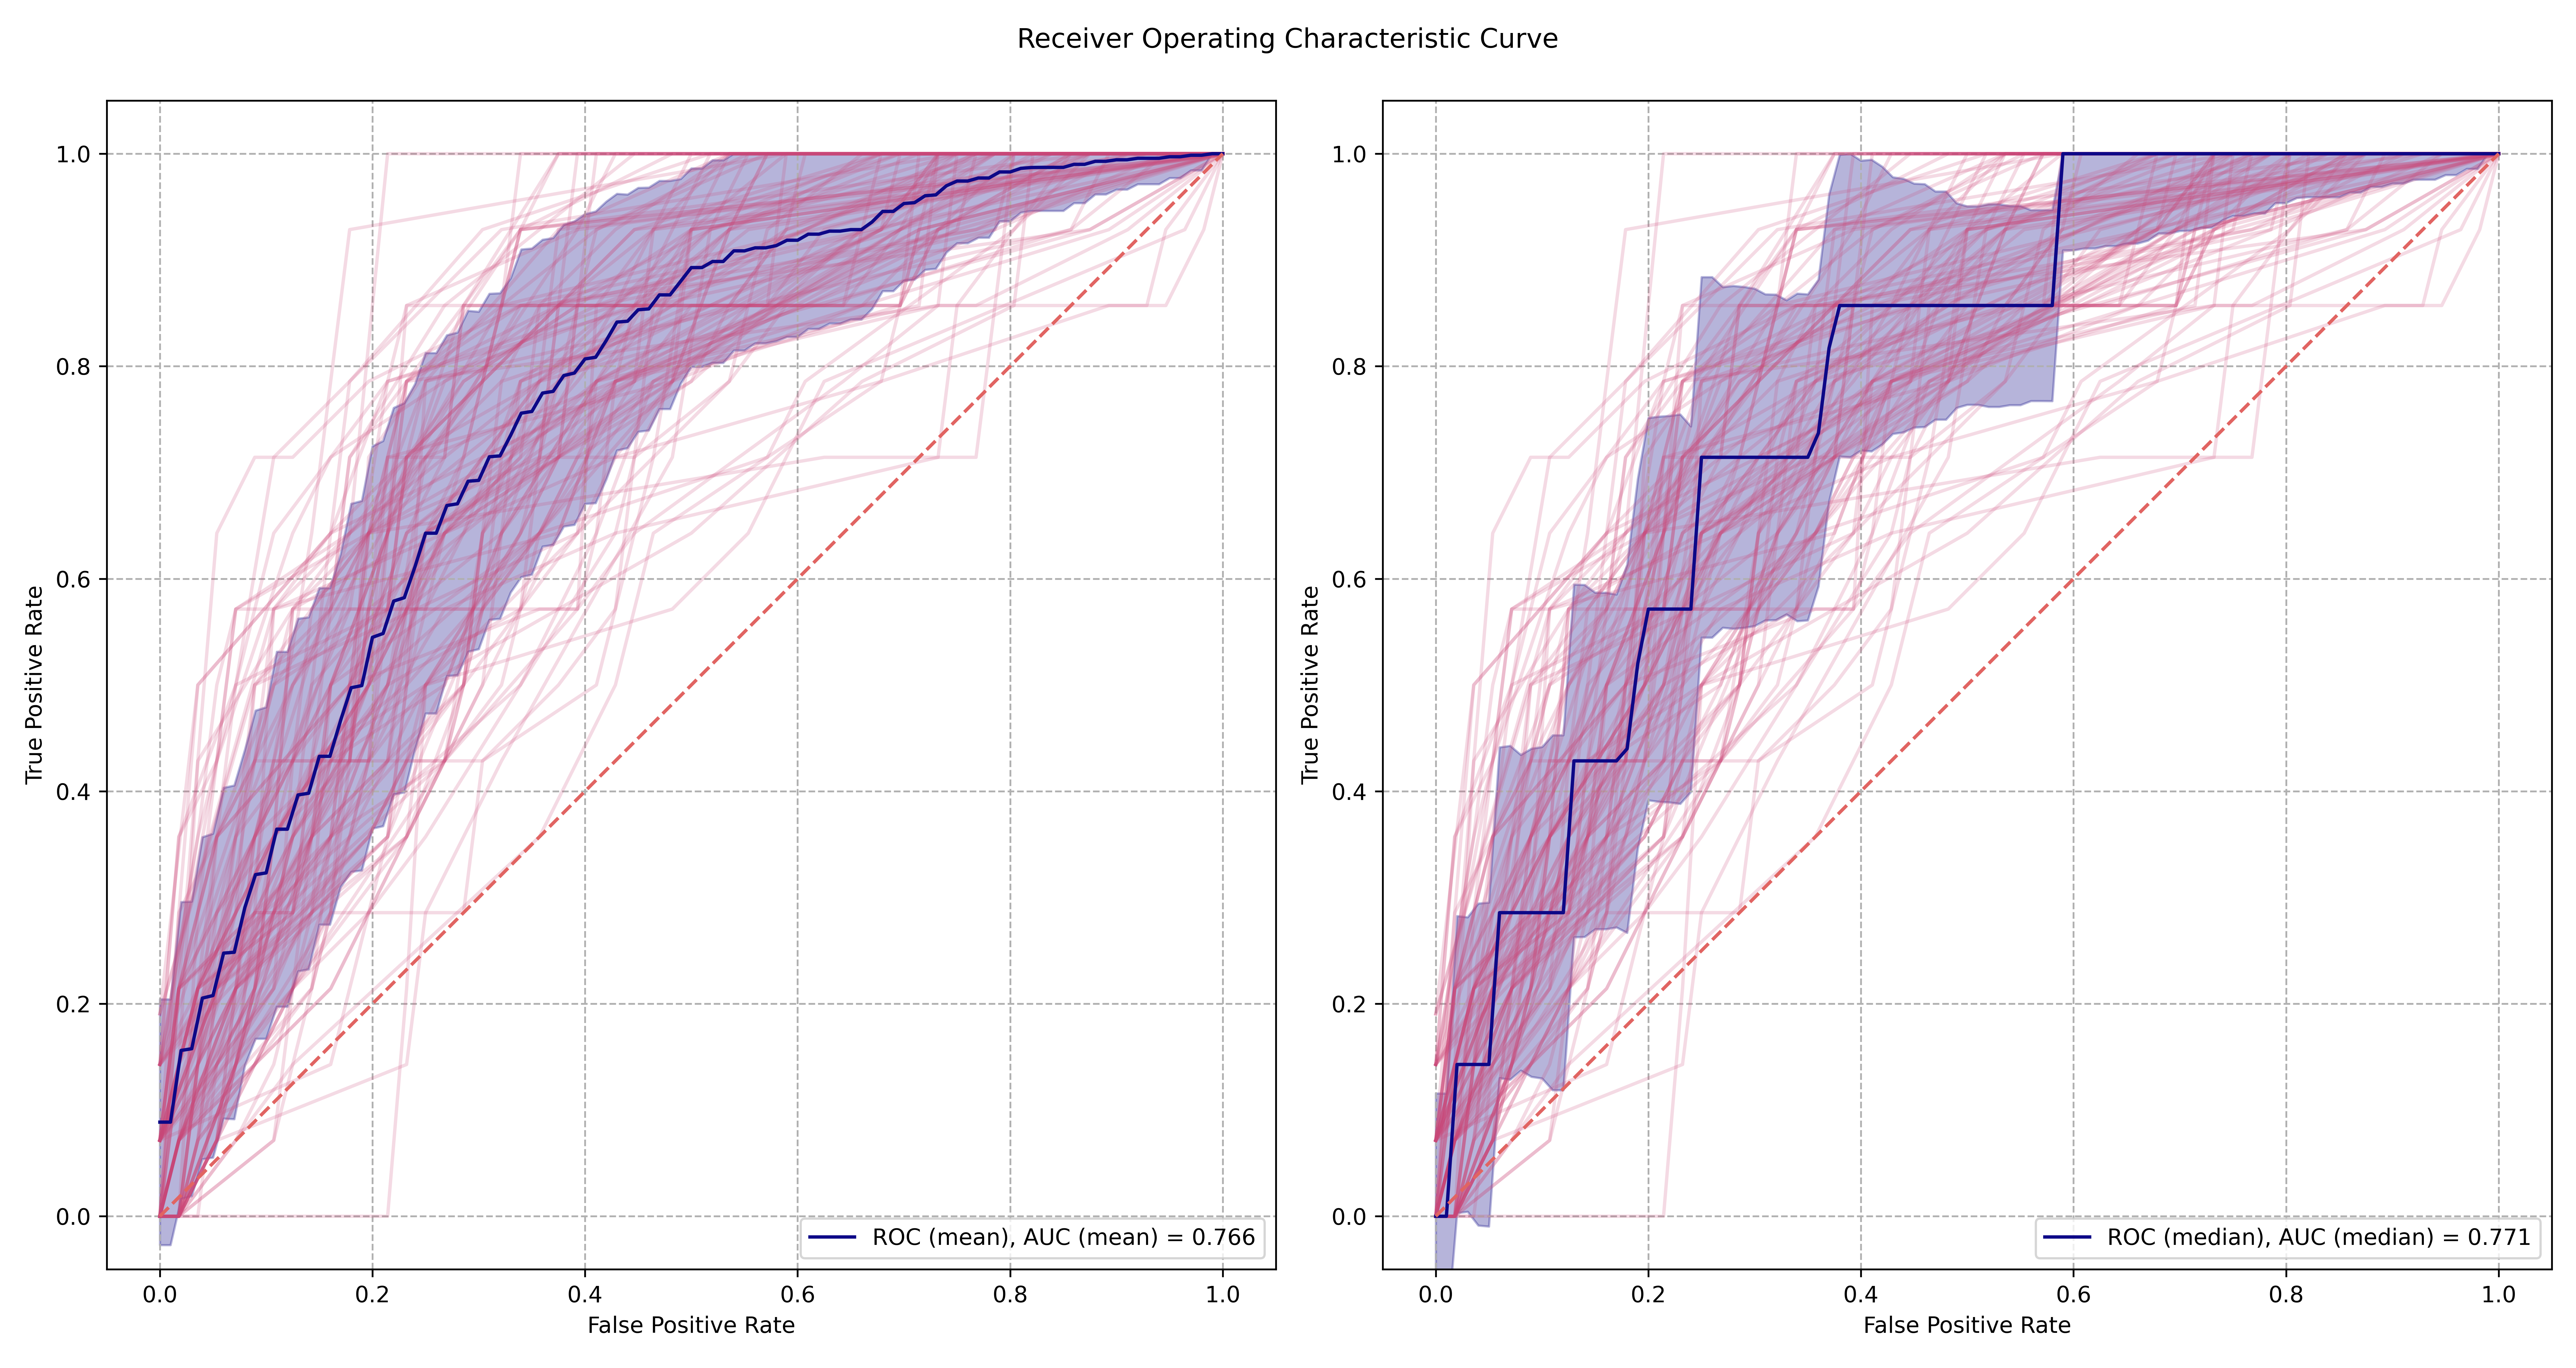
\includegraphics[width=\textwidth]{img/avg_roc.png}
    \caption{\ac{roc} curves for an importance filter level of \num{2.17280844256e-4}. Darker curves show the average, while the shading denotes standard deviation. Semitransparent curves show individual \acp{roc}.}\label{fig:avg_roc}
\end{figure}

% \subsection{Feature Grouping}

While features were treated as a single, all-containing set in the above 
classifications, grouping features shows clear differences in the effect of 
individual feature groups on a successful classification. \enquote{Synergy}
inside a grouping was measured by the ratio of the balanced accuracy the model
trained on that group reached (evaluated over 100 instances) to the average of
importance of features in that group. The importance was measured as described 
in Section~\ref{sec:filtering_importance}, comparing features against all 
available. Groupings deemed \enquote{synergetic} were those that achieved 
unusually high synergy. As expectations about differences in these synergy 
levels were unclear, an arbitrary condition has been chosen; synergy is 
\enquote{unusual} if lies outside the \SI{95}{\percent} confidence interval of
a linear regression over all groupings of the same category. It must be noted 
that there are grounds to suspect this methodology is flawed, as discussed in 
Section~\ref{sec:discussion}. Outlier groupings can be seen in 
Figure~\ref{fig:accuracy_vs_importance}, sitting outside the shaded area marking
the confidence interval.

\begin{figure}[H]
    \centering
    \makebox[\textwidth][c]{\includegraphics[width=1.15\textwidth]{img/accuracy_vs_importance.png}}
    \caption{The balanced accuracy per feature grouping in relation to that grouping's average importance per feature. Larger dots denote larger groups. The line represents a linear regression, with the lightly shaded area marking the \SI{95}{\percent} confidence interval. Groupings that fall outside the confidence interval are labelled in \textit{italics}. Labels for feature method groups have been omitted in favor of legibility. The full information these plots are based on can be found in the appendix under Section~\ref{sec:accuracy_vs_importance}.}\label{fig:accuracy_vs_importance}
\end{figure}



% TODO: Analyze the results further

% Plot Group Performance vs Avg Importance

%  Good    /  o
%      o  o
%        /   o
%   o   / o
%      /  o
%     / o  o Bad
% /\ Group performance
% -> Avg Importance


% Generate and plot AUC/ROC for best accuracy
\newpage{}
\section{Discussion}\label{sec:discussion}

This thesis has shown the construction and evaluation of \iac{rf}-based 
machine learning classifier for the prediction of \ac{pcr} in colorectal 
tumor patients. Considering the performance of this classifier, the 
prediction of \ac{pcr} through \ac{mri}-based radiomics features seems, on 
average, possible.

The assignment of a weighted average of importance to individual features helped
to improve the model. It must be considered that, as the testing set was involved in the selection of
features, results generated through the classification of this set may present
a biased evaluation of the total model performance. Due to its involvement in 
feature filtering, testing data was not completely \enquote{unknown} during the
construction of the classifier model. This suggests, that a more 
representative model accuracy can be obtained using a training/validation/test 
set split, as to not weigh feature selection in favor of a \enquote{known} 
test set~\cite{fundamentals_of_machine_learning}.

Although the usage of importance-based filtering raised the overall accuracy, the relation
between filter levels and model performance did not conform to 
expectations. As stated in Section~\ref{sec:hypothesis}, filtering by importance
was thought to immediately improve accuracy, as a large amount of unnecessary
or non-discriminative features was removed from the dataset. Instead, performance
climbed only with higher filter levels. Although more features were dropped than
initially expected, the number of features used is still significantly higher 
than in comparable studies. The filter level for optimal balanced accuracy 
leaves a set of 329 features, compared to the 30 identifiers used 
in~\cite{radiomics_analysis_pcr_rectal}, 18 used in~\cite{rectal_radiomics_svm_rf} 
and 4 used in~\cite{multisite_rectal_radiomics}. % TODO: Check this!!!!!!!!!1
As two of these studies~\cite{radiomics_analysis_pcr_rectal,rectal_radiomics_svm_rf} achieved higher \ac{auc} scores than the model created 
here, both at its best performance and with a significantly smaller feature set,
this may indicate the usage of a flawed feature selection method.
It must be noted, that both of these studies relied on classification methods,
that do not match \iac{rf} model exactly. When taking into consideration the
study with a matching classifier model,~\cite{multisite_rectal_radiomics}, a
similar \ac{auc} score was achieved\footnote{The classification scores for the model
presented in this thesis is a composite value. In a single model instance, both
better and worse results are possible.}, which calls this conclusion 
into question.

Another conflict arises in the determination of importances used here when 
compared to the performance of grouping-based models. Initially, it was assumed
that these metrics share a positive covariance, that is, a group of features 
deemed more important on average is expected to perform better together. 
If a linear relationship is assumed, the simple linear regression describing 
this relationship, as seen in Figure~\ref{fig:accuracy_vs_importance}, calls this
into question. While an equal number of positive and negative correlations show
up, none are statistically significant. 

Two possible conclusions are drawn here to possibly explain this unexpected 
behavior. Firstly, the metric of importance, as defined in the context of this
thesis, may not accurately describe how individual features contribute to the 
final result. An argument against this is posed by the improvement to model 
performance caused by importance-based filtering. Still, this improvement is not
proven to arise solely (or mostly) from the removal of less important features,
rather than from the reduction of features in general. The latter could be argued using
the conclusion of~\cite{considerations_of_sample_and_feature_size}, which 
states that an abundance in features in relation to training cases can 
negatively affect model performance.

Secondly, the possibility of an ill-fitting analysis. The connection between
group importance may exist, but not be accurately characterized by a simple 
linear regression. This would imply the necessity of using either 
non-linear regression or a more careful examination of outliers. Although this
circumstance is believed to be possible, its further exploration has been 
intentionally omitted in order to avoid accidental cherry-picking.

Having taken possible weaknesses of the metric defined in 
Section~\ref{sec:filtering_grouping} and used in the analysis of 
Figure~\ref{fig:accuracy_vs_importance} into consideration, its results may 
still be of interest in the classification of \ac{mri} imaging data.
When grouping features by the filter applied to the original imaging data, 
\enquote{\acp{lbp}} consistently achieve unexpectedly high synergy, both when measured by
mean and median importance. This is consistent with~\cite{local_binary_patterns},
which introduced this metric as a tool for the analysis of tissue texture.
Other filters such as \enquote{gradient} and \enquote{\ac{log}} achieved high synergy in either mean
or median importance analysis, but failed to reproduce this result in the other.
Wavelet filters, describing spatial frequencies across the input image, showed
consistently high synergy for \enquote{HLL}. Other wavelet configurations 
achieved unremarkable or even very low synergy. The only filters consistently 
resulting in a remarkably low synergy are \enquote{logarithm} and \enquote{squareroot}, along with 
the \enquote{original}, unfiltered image data.

When combining features by their respective feature group, as defined by 
PyRadiomics~\cite{py_rad}, the only groupings to stand out are \enquote{\ac{glrlm}}
and \enquote{shape}, performing better and worse than expected in one 
averaging category respectively. The low synergy in spite of high average 
importance in the \enquote{shape} group may indicate redundant information 
between members of that group. If so, individual features may achieve a high
importance on their own, but do worse than expected in combination. Should this
be true, it calls the effectiveness of the annotation interpolation algorithm
used in this thesis (see Section~\ref{sec:3d_and_2d}) into question.

Both because of this category's large amount of groups and of the regression's
comparatively small confidence interval, grouping by feature extraction method
shows an unusual amount of outliers. In fact, the vast majority of available 
groupings, measured by both mean and median importance, are outliers, with 
80 and 76 groupings out of a total of 99 respectively. Generally, outliers
above the confidence interval largely consist of texture-based features, 
agreeing in part with the earlier groupings categories. In general, texture
features appear to be important for successful classification, both in agreement
with the findings of this thesis and with earlier works~\cite{rectal_radiomics_svm_rf,radiomics_analysis_pcr_rectal}.
In contrast, shape-based
features dominate positions of high average importance but low synergy. This
 may lead to the assumption, that these features do not hold relevant 
information for classification. It must be considered though, that due to 
the non-existence of annotation-based filters, these groups largely consist of
a single feature. 

The grouping of features by category has shown groupings of both high accuracy
and high synergy. Though no grouping has achieved better accuracy than the 
overall model, as described in Section~\ref{sec:filtering_importance}, groupings
like \enquote{lbp-3D-m1} or \enquote{ZonePercentage} show significant performance with both a smaller 
feature count and low assigned \enquote{importance}. This may indicate the 
possibility of higher model accuracy and improved build duration through the
choice of a more rigorous feature selection method.

Overall, a model that, on average, successfully predicts \ac{pcr} has been 
constructed. Although techniques to improve model accuracy have been 
implemented, their exact effects are not yet fully understood and require further 
investigation.

% Write about (un)expected importance/accuracy (in-)coherence

% TODO: Go over bib.bib. Make sure titles are enclosed in {}

\newpage{}
\printbibliography[heading=bibnumbered]
\lhead{}
% !TEX program = xelatex

\section{Glossary}

% Leave some space between acronym and definition
\begin{acronym}[AAAAAAAAAAAA]
    \acro{auc}[AUC]{Area Under the Curve}
    \acrodefindefinite{auc}{an}{a}
    \acro{collage}[CoLlAGe]{Co-occurrence of Local Anisotropic Gradient Orientations}
    \acro{ct}[CT]{Computed Tomography}
    \acro{dl}[DL]{Deep-Learning}
    \acro{dwi}[DWI]{Diffusion Weighted Imaging}
    \acro{fn}[FN]{False Negative}
    \acrodefindefinite{fn}{an}{a}
    \acro{fp}[FP]{False Positive}
    \acrodefindefinite{fp}{an}{a}
    \acro{fpr}[FPR]{False Positive Rate}
    \acro{glcm}[GLCM]{Gray Level Cooccurence Matrix}
    \acro{gldm}[GLDM]{Gray Level Dependence Matrix}
    \acro{glrlm}[GLRLM]{Gray Level Run Length Matrix}
    \acro{glszm}[GLSZM]{Gray Level Size Zone Matrix}
    \acro{ibsi}[IBSI]{Image Biomarker Standardisation Initiative}
    \acrodefindefinite{ibsi}{an}{a}
    \acro{lasso}[LASSO]{Least Absolute Shrinkage and Selection Operator}
    \acro{lbp}[LBP]{Local Binary Pattern}
    \acro{log}[LoG]{Laplacian of Gaussian}
    \acro{mri}[MRI]{Magnetic Resonance Imaging}
    \acrodefindefinite{mri}{an}{a}
    \acro{ngldm}[NGLDM]{Neighboring Gray Level Dependence Matrix}
    \acro{ngtdm}[NGTDM]{Neighboring Gray Tone Difference Matrix}
    %\acro{mrmr}[mRMR]{Minimum Redundancy Maximum Relevance}
    %\acrodefindefinite{mrmr}{an}{a}
    \acro{pcr}[pCR]{Pathological Complete Remission}
    \acro{pd}[PD]{Proton Density}
    \acro{pet}[PET]{Positron Emission Tomography}
    \acro{rf}[RF]{Random Forest}
    \acrodefindefinite{rf}{an}{a}
    \acro{roc}[ROC]{Receiver Operating Characteristic}
    \acrodefindefinite{roc}{an}{a}
    \acro{roi}[ROI]{Region of Interest}
    \acrodefindefinite{roi}{an}{a}
    \acroplural{roi}[ROIs]{Regions of Interest}
    \acro{salk}[SALK]{Salzburger Landeskliniken}
    \acro{svm}[SVM]{Support Vector Machine}
    \acrodefindefinite{svm}{an}{a}
    \acro{te}[TE]{Echo Time}
    \acro{tn}[TN]{True Negative}
    \acro{tnr}[TNR]{True Negative Rate}
    \acro{tp}[TP]{True Positive}
    \acro{tpr}[TPR]{True Positive Rate}
    \acro{tr}[TR]{Repetition Time}
\end{acronym}
\section{Appendix}

This section contains complimentary details to information introduced in the 
main body of this thesis. It is referred to, if data provided here may 
potentially, but not necessarily, be relevant to the reader.

\subsection{Additional MRI Image Credit}

To illustrate the difference between weightings in \ac{mri} scans, a comparison 
between T\textsubscript{1} and T\textsubscript{2} weighted images of a human 
brain were shown in Figure~\ref{fig:t1_t2}.
Data were provided in part by the Human Connectome Project, WU-Minn Consortium 
(Principal Investigators: David Van Essen and Kamil Ugurbil; 1U54MH091657) 
funded by the 16 NIH Institutes and Centers that support the NIH Blueprint for 
Neuroscience Research; and by the McDonnell Center for Systems Neuroscience at 
Washington University. The \ac{mri} scan in question was taken of patient 100206.

\subsection{PyRadiomics Extractor Configuration}\label{sec:pyrad_config}

The configuration in Listing~\ref{code:pyrad_config} is supplied to PyRadiomics' 
\texttt{radiomics.featureextractor.RadiomicsFeatureExtractor} class, providing 
extraction parameters. 

\begin{lstlisting}[caption={PyRadiomics configuration file. This file is based on the default PyRadiomics configuration file\cite{py_rad_docs}. The majority of features is enabled, to be selectively filtered out later. Some features are disabled, as recommended in the PyRadiomics documentation. Examples for reasons to disable certain features are obsolescense or redundance in combination with other features~\cite{py_rad_docs}}., label={code:pyrad_config}]
    setting:
    binWidth: 25
    label: 1
    interpolator: sitkBSpline
    resampledPixelSpacing: null
    weightingNorm: null
    normalize: true
  imageType:
    Original: {}
    LoG:
      sigma:
        - 1
        - 3
    Wavelet:
      binWidth: 10
    Square: {}
    SquareRoot: {}
    Logarithm: {}
    Exponential: {}
    Gradient: {}
    LBP3D: {}
  featureClass:
    shape: null
    firstorder: []
    glcm:
      - Autocorrelation
      - JointAverage
      - ClusterProminence
      - ClusterShade
      - ClusterTendency
      - Contrast
      - Correlation
      - DifferenceAverage
      - DifferenceEntropy
      - DifferenceVariance
      - JointEnergy
      - JointEntropy
      - Imc1
      - Imc2
      - Idm
      - Idmn
      - Id
      - Idn
      - InverseVariance
      - MaximumProbability
      - SumEntropy
      - SumSquares
    glrlm: null
    glszm: null
    gldm: null
    ngtdm: null  
\end{lstlisting}

\subsection{Software Versions}

The experimental setup presented here depends on a collection of software 
distributions. To enable replication of this setup, the versions of all relevant
tools are listed in Table~\ref{tbl:software_versions}, where 
Table~\ref{tbl:library_versions} gives information about individual software 
libraries used in conjunction with the Python programming language.

\begin{table}[H]
  \begin{tabularx}{\textwidth}{X r}
    Software & Version\\\hline
    Python & 3.9.7 \\
    ITK-SNAP & 3.8.0 \\
  \end{tabularx}
  \caption{Versions of Software Tools used in the development of this thesis. 
  Tools that do not have a direct impact on model performance and which are not 
  specifically referenced, such as text editors, are omitted.}\label{tbl:software_versions}
\end{table}

\begin{table}[H]
  \begin{tabularx}{\textwidth}{X r}
    Library & Version \\\hline
    cycler & 0.10.0 \\
    docopt & 0.6.2 \\
    imageio & 2.9.0 \\
    joblib & 1.0.1 \\
    kiwisolver & 1.3.2 \\
    matplotlib & 3.4.3 \\
    networkx & 2.6.2 \\
    nibabel & 3.2.1 \\
    numpy & 1.21.2 \\
    packaging & 21.0 \\
    Pillow & 8.4.0 \\
    pykwalify & 1.8.0 \\
    pyparsing & 2.4.7 \\
    pyradiomics & 3.0.1 \\
    python-dateutil & 2.8.2 \\
    PyWavelets & 1.1.1 \\
    ruamel.yaml & 0.17.14 \\
    ruamel.yaml.clib & 0.2.6 \\
    scikit-image & 0.18.3 \\
    scikit-learn & 0.24.2 \\
    scipy & 1.7.1 \\
    SimpleITK & 2.1.0 \\
    six & 1.16.0 \\
    sklearn & 0.0 \\
    threadpoolctl & 2.2.0 \\
    tifffile & 2021.8.8 \\
  \end{tabularx}
  \caption{Versions of Python libraries used in the development of this thesis.}\label{tbl:library_versions}
\end{table}

\subsection{\acs{mri} Metadata}\label{sec:mri_metadata}

Here, additional information the \ac{mri} scans making up the total dataset
is provided. All \ac{mri} scans have been T\textsubscript{2} weighted, with a
\SI[minimum-decimal-digits=0,drop-zero-decimal]{16}{bit} color depth. Information about Voxel and Scan dimensions can be 
found in Table~\ref{tbl:scan_dimensions}.

\sisetup{group-digits=integer,round-mode=places,round-precision=8}

\begin{table}[H]
  \tiny
  \begin{tabularx}{\textwidth}{X X r}
    Voxel Dimensions & Scan Dimensions & Number of Scans \\\hline
    \num{0.4225352} $ \times $ \num{0.4225352} $ \times $ \num{3.86}         &   \num[minimum-decimal-digits=0,drop-zero-decimal]{640} $ \times $ \num[minimum-decimal-digits=0,drop-zero-decimal]{640} $ \times $ \num[minimum-decimal-digits=0,drop-zero-decimal]{25}  & 34\\
    \num{0.33854166} $ \times $ \num{0.33854166} $ \times $ \num{3.85}       &   \num[minimum-decimal-digits=0,drop-zero-decimal]{768} $ \times $ \num[minimum-decimal-digits=0,drop-zero-decimal]{768} $ \times $ \num[minimum-decimal-digits=0,drop-zero-decimal]{26}  & 9\\
    \num{0.875} $ \times $ \num{0.875} $ \times $ \num{3.75}                 &   \num[minimum-decimal-digits=0,drop-zero-decimal]{320} $ \times $ \num[minimum-decimal-digits=0,drop-zero-decimal]{320} $ \times $ \num[minimum-decimal-digits=0,drop-zero-decimal]{38}  & 5\\
    \num{0.4882813} $ \times $ \num{0.4882813} $ \times $ \num{5.2}          &   \num[minimum-decimal-digits=0,drop-zero-decimal]{512} $ \times $ \num[minimum-decimal-digits=0,drop-zero-decimal]{512} $ \times $ \num[minimum-decimal-digits=0,drop-zero-decimal]{22}  & 3\\
    \num{0.4882813} $ \times $ \num{0.4882813} $ \times $ \num{5.2000003}    &   \num[minimum-decimal-digits=0,drop-zero-decimal]{512} $ \times $ \num[minimum-decimal-digits=0,drop-zero-decimal]{512} $ \times $ \num[minimum-decimal-digits=0,drop-zero-decimal]{22}  & 3\\
    \num{0.625} $ \times $ \num{0.625} $ \times $ \num{3.75}                 &   \num[minimum-decimal-digits=0,drop-zero-decimal]{384} $ \times $ \num[minimum-decimal-digits=0,drop-zero-decimal]{512} $ \times $ \num[minimum-decimal-digits=0,drop-zero-decimal]{34}  & 3\\
    \num{0.75} $ \times $ \num{0.75} $ \times $ \num{4.4}                    &   \num[minimum-decimal-digits=0,drop-zero-decimal]{320} $ \times $ \num[minimum-decimal-digits=0,drop-zero-decimal]{320} $ \times $ \num[minimum-decimal-digits=0,drop-zero-decimal]{40}  & 3\\
    \num{0.3125} $ \times $ \num{0.3125} $ \times $ \num{3.5}                &   \num[minimum-decimal-digits=0,drop-zero-decimal]{768} $ \times $ \num[minimum-decimal-digits=0,drop-zero-decimal]{768} $ \times $ \num[minimum-decimal-digits=0,drop-zero-decimal]{36}  & 2\\
    \num{0.31413612} $ \times $ \num{0.31413612} $ \times $ \num{3.85}       &   \num[minimum-decimal-digits=0,drop-zero-decimal]{864} $ \times $ \num[minimum-decimal-digits=0,drop-zero-decimal]{864} $ \times $ \num[minimum-decimal-digits=0,drop-zero-decimal]{30}  & 2\\
    \num{0.33854166} $ \times $ \num{0.33854166} $ \times $ \num{3.8500001}  &   \num[minimum-decimal-digits=0,drop-zero-decimal]{768} $ \times $ \num[minimum-decimal-digits=0,drop-zero-decimal]{768} $ \times $ \num[minimum-decimal-digits=0,drop-zero-decimal]{26}  & 2\\
    \num{0.625} $ \times $ \num{0.625} $ \times $ \num{5.0}                  &   \num[minimum-decimal-digits=0,drop-zero-decimal]{384} $ \times $ \num[minimum-decimal-digits=0,drop-zero-decimal]{512} $ \times $ \num[minimum-decimal-digits=0,drop-zero-decimal]{26}  & 2\\
    \num{0.6510417} $ \times $ \num{0.6510417} $ \times $ \num{3.3}          &   \num[minimum-decimal-digits=0,drop-zero-decimal]{384} $ \times $ \num[minimum-decimal-digits=0,drop-zero-decimal]{384} $ \times $ \num[minimum-decimal-digits=0,drop-zero-decimal]{30}  & 2\\
    \num{0.78125} $ \times $ \num{0.78125} $ \times $ \num{6.5}              &   \num[minimum-decimal-digits=0,drop-zero-decimal]{320} $ \times $ \num[minimum-decimal-digits=0,drop-zero-decimal]{320} $ \times $ \num[minimum-decimal-digits=0,drop-zero-decimal]{25}  & 2\\
    \num{0.9375} $ \times $ \num{0.9375} $ \times $ \num{3.6000001}          &   \num[minimum-decimal-digits=0,drop-zero-decimal]{320} $ \times $ \num[minimum-decimal-digits=0,drop-zero-decimal]{320} $ \times $ \num[minimum-decimal-digits=0,drop-zero-decimal]{30}  & 2\\
    \num{0.31413612} $ \times $ \num{0.31413612} $ \times $ \num{3.8499997}  &   \num[minimum-decimal-digits=0,drop-zero-decimal]{864} $ \times $ \num[minimum-decimal-digits=0,drop-zero-decimal]{864} $ \times $ \num[minimum-decimal-digits=0,drop-zero-decimal]{30}  & 1\\
    \num{0.33678755} $ \times $ \num{0.33678755} $ \times $ \num{3.85}       &   \num[minimum-decimal-digits=0,drop-zero-decimal]{800} $ \times $ \num[minimum-decimal-digits=0,drop-zero-decimal]{800} $ \times $ \num[minimum-decimal-digits=0,drop-zero-decimal]{26}  & 1\\
    \num{0.33854166} $ \times $ \num{0.33854166} $ \times $ \num{3.8499997}  &   \num[minimum-decimal-digits=0,drop-zero-decimal]{768} $ \times $ \num[minimum-decimal-digits=0,drop-zero-decimal]{768} $ \times $ \num[minimum-decimal-digits=0,drop-zero-decimal]{26}  & 1\\
    \num{0.390625} $ \times $ \num{0.390625} $ \times $ \num{4.4}            &   \num[minimum-decimal-digits=0,drop-zero-decimal]{512} $ \times $ \num[minimum-decimal-digits=0,drop-zero-decimal]{512} $ \times $ \num[minimum-decimal-digits=0,drop-zero-decimal]{23}  & 1\\
    \num{0.4225352} $ \times $ \num{0.4225352} $ \times $ \num{3.8599997}    &   \num[minimum-decimal-digits=0,drop-zero-decimal]{640} $ \times $ \num[minimum-decimal-digits=0,drop-zero-decimal]{640} $ \times $ \num[minimum-decimal-digits=0,drop-zero-decimal]{25}  & 1\\
    \num{0.4225352} $ \times $ \num{0.4225352} $ \times $ \num{3.8600001}    &   \num[minimum-decimal-digits=0,drop-zero-decimal]{640} $ \times $ \num[minimum-decimal-digits=0,drop-zero-decimal]{640} $ \times $ \num[minimum-decimal-digits=0,drop-zero-decimal]{25}  & 1\\
    \num{0.42857143} $ \times $ \num{0.42857143} $ \times $ \num{3.86}       &   \num[minimum-decimal-digits=0,drop-zero-decimal]{560} $ \times $ \num[minimum-decimal-digits=0,drop-zero-decimal]{560} $ \times $ \num[minimum-decimal-digits=0,drop-zero-decimal]{25}  & 1\\
    \num{0.4375} $ \times $ \num{0.4375} $ \times $ \num{5.2000003}          &   \num[minimum-decimal-digits=0,drop-zero-decimal]{512} $ \times $ \num[minimum-decimal-digits=0,drop-zero-decimal]{512} $ \times $ \num[minimum-decimal-digits=0,drop-zero-decimal]{22}  & 1\\
    \num{0.4882813} $ \times $ \num{0.4882813} $ \times $ \num{5.1999993}    &   \num[minimum-decimal-digits=0,drop-zero-decimal]{512} $ \times $ \num[minimum-decimal-digits=0,drop-zero-decimal]{512} $ \times $ \num[minimum-decimal-digits=0,drop-zero-decimal]{22}  & 1\\
    \num{0.5078125} $ \times $ \num{0.5078125} $ \times $ \num{5.2}          &   \num[minimum-decimal-digits=0,drop-zero-decimal]{512} $ \times $ \num[minimum-decimal-digits=0,drop-zero-decimal]{512} $ \times $ \num[minimum-decimal-digits=0,drop-zero-decimal]{22}  & 1\\
    \num{0.520833} $ \times $ \num{0.520833} $ \times $ \num{3.6000042}      &   \num[minimum-decimal-digits=0,drop-zero-decimal]{384} $ \times $ \num[minimum-decimal-digits=0,drop-zero-decimal]{384} $ \times $ \num[minimum-decimal-digits=0,drop-zero-decimal]{25}  & 1\\
    \num{0.5273438} $ \times $ \num{0.5273438} $ \times $ \num{5.0}          &   \num[minimum-decimal-digits=0,drop-zero-decimal]{512} $ \times $ \num[minimum-decimal-digits=0,drop-zero-decimal]{512} $ \times $ \num[minimum-decimal-digits=0,drop-zero-decimal]{23}  & 1\\
    \num{0.5445545} $ \times $ \num{0.5445545} $ \times $ \num{4.4}          &   \num[minimum-decimal-digits=0,drop-zero-decimal]{512} $ \times $ \num[minimum-decimal-digits=0,drop-zero-decimal]{512} $ \times $ \num[minimum-decimal-digits=0,drop-zero-decimal]{28}  & 1\\
    \num{0.625} $ \times $ \num{0.625} $ \times $ \num{3.8500001}            &   \num[minimum-decimal-digits=0,drop-zero-decimal]{512} $ \times $ \num[minimum-decimal-digits=0,drop-zero-decimal]{512} $ \times $ \num[minimum-decimal-digits=0,drop-zero-decimal]{30}  & 1\\
    \num{0.71875} $ \times $ \num{0.71875} $ \times $ \num{3.6}              &   \num[minimum-decimal-digits=0,drop-zero-decimal]{320} $ \times $ \num[minimum-decimal-digits=0,drop-zero-decimal]{320} $ \times $ \num[minimum-decimal-digits=0,drop-zero-decimal]{27}  & 1\\
    \num{0.71875} $ \times $ \num{0.71875} $ \times $ \num{4.8}              &   \num[minimum-decimal-digits=0,drop-zero-decimal]{320} $ \times $ \num[minimum-decimal-digits=0,drop-zero-decimal]{320} $ \times $ \num[minimum-decimal-digits=0,drop-zero-decimal]{28}  & 1\\
    \num{0.78125} $ \times $ \num{0.78125} $ \times $ \num{3.6000001}        &   \num[minimum-decimal-digits=0,drop-zero-decimal]{320} $ \times $ \num[minimum-decimal-digits=0,drop-zero-decimal]{320} $ \times $ \num[minimum-decimal-digits=0,drop-zero-decimal]{27}  & 1\\
    \num{0.78125} $ \times $ \num{0.78125} $ \times $ \num{6.0}              &   \num[minimum-decimal-digits=0,drop-zero-decimal]{320} $ \times $ \num[minimum-decimal-digits=0,drop-zero-decimal]{320} $ \times $ \num[minimum-decimal-digits=0,drop-zero-decimal]{30}  & 1\\
    \num{0.9765625} $ \times $ \num{0.9765625} $ \times $ \num{6.25}         &   \num[minimum-decimal-digits=0,drop-zero-decimal]{256} $ \times $ \num[minimum-decimal-digits=0,drop-zero-decimal]{256} $ \times $ \num[minimum-decimal-digits=0,drop-zero-decimal]{19}  & 1\\       
  \end{tabularx}
  \caption{Voxel and scan dimensions along with the number of scans conforming to these dimensions.}\label{tbl:scan_dimensions}
\end{table}

\sisetup{round-mode=none}

\subsection{Grouping Accuracy versus Grouping Importance}\label{sec:accuracy_vs_importance}

This data makes up the base of Figure~\ref{fig:accuracy_vs_importance}. Data points are
sectioned into three groupings; grouping by input image filter, by feature group
and by feature extraction method.
The theory behind these groupings is covered in detail in Section~\ref{sec:filtering_grouping}.

Outliers, listed in Section~\ref{sec:appendix_outliers}, denote feature 
groupings that are either unexpectedly \enquote{synergetic}, or unusually not 
so. An outlier is defined as being located outside the \SI{95}{\percent} 
confidence interval of a linear regression of accuracy over average importance 
per feature, fitted over all groupings of that category.

\subsubsection{Outliers}\label{sec:appendix_outliers}

Table~\ref{tbl:outliers} lists all feature groupings that performed either 
significantly better or worse than expected. The table contains groupings of 
all categories. Groupings split by category along with the exact values of 
both average importance and accuracy of that grouping can be found in the 
following section.

{\tiny
\begin{xltabular}{\textwidth}{X l l r}
    \caption{Groupings with unusually high or low \enquote{synergy}. Those outside a \SI{95}{\percent} Confidence Interval are considered outliers, where those performing better than expected are marked as \enquote{Above}, while those performing worse than expected are labelled \enquote{Below}.}\label{tbl:outliers}\endlastfoot\\
Grouping Category & Average Function & Position relative to Confidence Interval & Name of Grouping \\\hline\endhead
By Input Filter & Mean & Below & squareroot \\
By Input Filter & Mean & Below & original \\
By Input Filter & Mean & Below & logarithm \\
By Input Filter & Mean & Below & log-sigma-1-0-mm-3D \\
By Input Filter & Mean & Below & wavelet-LLL \\

By Input Filter & Mean & Above & wavelet-LHL \\
By Input Filter & Mean & Above & gradient \\
By Input Filter & Mean & Above & lbp-3D-m1 \\
By Input Filter & Mean & Above & wavelet-HLL \\

By Input Filter & Median & Below & squareroot \\
By Input Filter & Median & Below & original \\
By Input Filter & Median & Below & logarithm \\
By Input Filter & Median & Below & wavelet-LLL \\

By Input Filter & Median & Above & log-sigma-3-0-mm-3D \\
By Input Filter & Median & Above & wavelet-HHL \\
By Input Filter & Median & Above & wavelet-LHL \\
By Input Filter & Median & Above & lbp-3D-m1 \\
By Input Filter & Median & Above & wavelet-HLL \\

By Feature Group & Mean & Below & shape \\

By Feature Group & Median & Above & glrlm \\

By Feature Extraction Method & Mean & Below & Flatness \\
By Feature Extraction Method & Mean & Below & Maximum3DDiameter \\
By Feature Extraction Method & Mean & Below & DependenceVariance \\
By Feature Extraction Method & Mean & Below & RunLengthNonUniformityNormalized \\
By Feature Extraction Method & Mean & Below & SurfaceVolumeRatio \\
By Feature Extraction Method & Mean & Below & Skewness \\
By Feature Extraction Method & Mean & Below & InterquartileRange \\
By Feature Extraction Method & Mean & Below & MeanAbsoluteDeviation \\
By Feature Extraction Method & Mean & Below & RootMeanSquared \\
By Feature Extraction Method & Mean & Below & Maximum2DDiameterColumn \\
By Feature Extraction Method & Mean & Below & Sphericity \\
By Feature Extraction Method & Mean & Below & LargeDependenceEmphasis \\
By Feature Extraction Method & Mean & Below & DifferenceVariance \\
By Feature Extraction Method & Mean & Below & Imc2 \\
By Feature Extraction Method & Mean & Below & SizeZoneNonUniformityNormalized \\
By Feature Extraction Method & Mean & Below & MajorAxisLength \\
By Feature Extraction Method & Mean & Below & LeastAxisLength \\
By Feature Extraction Method & Mean & Below & Maximum2DDiameterSlice \\
By Feature Extraction Method & Mean & Below & 90Percentile \\
By Feature Extraction Method & Mean & Below & JointEnergy \\
By Feature Extraction Method & Mean & Below & Variance \\
By Feature Extraction Method & Mean & Below & Mean \\
By Feature Extraction Method & Mean & Below & MaximumProbability \\
By Feature Extraction Method & Mean & Below & RunPercentage \\
By Feature Extraction Method & Mean & Below & HighGrayLevelRunEmphasis \\
By Feature Extraction Method & Mean & Below & DifferenceEntropy \\
By Feature Extraction Method & Mean & Below & RobustMeanAbsoluteDeviation \\
By Feature Extraction Method & Mean & Below & MinorAxisLength \\
By Feature Extraction Method & Mean & Below & Maximum2DDiameterRow \\
By Feature Extraction Method & Mean & Below & ShortRunHighGrayLevelEmphasis \\
By Feature Extraction Method & Mean & Below & JointEntropy \\
By Feature Extraction Method & Mean & Below & SurfaceArea \\
By Feature Extraction Method & Mean & Below & ShortRunEmphasis \\
By Feature Extraction Method & Mean & Below & LargeDependenceHighGrayLevelEmphasis \\

By Feature Extraction Method & Mean & Above & Busyness \\
By Feature Extraction Method & Mean & Above & LongRunLowGrayLevelEmphasis \\
By Feature Extraction Method & Mean & Above & SmallAreaHighGrayLevelEmphasis \\
By Feature Extraction Method & Mean & Above & GrayLevelNonUniformityNormalized \\
By Feature Extraction Method & Mean & Above & RunVariance \\
By Feature Extraction Method & Mean & Above & InverseVariance \\
By Feature Extraction Method & Mean & Above & VoxelVolume \\
By Feature Extraction Method & Mean & Above & Range \\
By Feature Extraction Method & Mean & Above & Contrast \\
By Feature Extraction Method & Mean & Above & Autocorrelation \\
By Feature Extraction Method & Mean & Above & SmallAreaLowGrayLevelEmphasis \\
By Feature Extraction Method & Mean & Above & SizeZoneNonUniformity \\
By Feature Extraction Method & Mean & Above & LongRunHighGrayLevelEmphasis \\
By Feature Extraction Method & Mean & Above & LargeAreaEmphasis \\
By Feature Extraction Method & Mean & Above & DifferenceAverage \\
By Feature Extraction Method & Mean & Above & GrayLevelNonUniformity \\
By Feature Extraction Method & Mean & Above & Coarseness \\
By Feature Extraction Method & Mean & Above & DependenceNonUniformityNormalized \\
By Feature Extraction Method & Mean & Above & DependenceNonUniformity \\
By Feature Extraction Method & Mean & Above & SmallDependenceLowGrayLevelEmphasis \\
By Feature Extraction Method & Mean & Above & MeshVolume \\
By Feature Extraction Method & Mean & Above & ZoneEntropy \\
By Feature Extraction Method & Mean & Above & ClusterProminence \\
By Feature Extraction Method & Mean & Above & GrayLevelVariance \\
By Feature Extraction Method & Mean & Above & Minimum \\
By Feature Extraction Method & Mean & Above & Energy \\
By Feature Extraction Method & Mean & Above & Elongation \\
By Feature Extraction Method & Mean & Above & Strength \\
By Feature Extraction Method & Mean & Above & Complexity \\
By Feature Extraction Method & Mean & Above & Idmn \\
By Feature Extraction Method & Mean & Above & RunEntropy \\
By Feature Extraction Method & Mean & Above & SumEntropy \\
By Feature Extraction Method & Mean & Above & Id \\
By Feature Extraction Method & Mean & Above & LargeAreaHighGrayLevelEmphasis \\
By Feature Extraction Method & Mean & Above & TotalEnergy \\
By Feature Extraction Method & Mean & Above & Idn \\
By Feature Extraction Method & Mean & Above & LargeAreaLowGrayLevelEmphasis \\
By Feature Extraction Method & Mean & Above & LongRunEmphasis \\
By Feature Extraction Method & Mean & Above & ZonePercentage \\
By Feature Extraction Method & Mean & Above & Median \\
By Feature Extraction Method & Mean & Above & SmallAreaEmphasis \\
By Feature Extraction Method & Mean & Above & ZoneVariance \\
By Feature Extraction Method & Mean & Above & ClusterTendency \\
By Feature Extraction Method & Mean & Above & Idm \\
By Feature Extraction Method & Mean & Above & DependenceEntropy \\
By Feature Extraction Method & Mean & Above & 10Percentile \\

By Feature Extraction Method & Median & Below & Flatness \\
By Feature Extraction Method & Median & Below & Maximum3DDiameter \\
By Feature Extraction Method & Median & Below & DependenceVariance \\
By Feature Extraction Method & Median & Below & RunLengthNonUniformityNormalized \\
By Feature Extraction Method & Median & Below & SurfaceVolumeRatio \\
By Feature Extraction Method & Median & Below & Skewness \\
By Feature Extraction Method & Median & Below & LowGrayLevelRunEmphasis \\
By Feature Extraction Method & Median & Below & InterquartileRange \\
By Feature Extraction Method & Median & Below & MeanAbsoluteDeviation \\
By Feature Extraction Method & Median & Below & RootMeanSquared \\
By Feature Extraction Method & Median & Below & Maximum2DDiameterColumn \\
By Feature Extraction Method & Median & Below & Sphericity \\
By Feature Extraction Method & Median & Below & LargeDependenceEmphasis \\
By Feature Extraction Method & Median & Below & DifferenceVariance \\
By Feature Extraction Method & Median & Below & Imc2 \\
By Feature Extraction Method & Median & Below & SizeZoneNonUniformityNormalized \\
By Feature Extraction Method & Median & Below & MajorAxisLength \\
By Feature Extraction Method & Median & Below & LowGrayLevelZoneEmphasis \\
By Feature Extraction Method & Median & Below & LeastAxisLength \\
By Feature Extraction Method & Median & Below & Maximum2DDiameterSlice \\
By Feature Extraction Method & Median & Below & 90Percentile \\
By Feature Extraction Method & Median & Below & JointEnergy \\
By Feature Extraction Method & Median & Below & Variance \\
By Feature Extraction Method & Median & Below & Mean \\
By Feature Extraction Method & Median & Below & MaximumProbability \\
By Feature Extraction Method & Median & Below & RunPercentage \\
By Feature Extraction Method & Median & Below & Imc1 \\
By Feature Extraction Method & Median & Below & HighGrayLevelRunEmphasis \\
By Feature Extraction Method & Median & Below & DifferenceEntropy \\
By Feature Extraction Method & Median & Below & RobustMeanAbsoluteDeviation \\
By Feature Extraction Method & Median & Below & MinorAxisLength \\
By Feature Extraction Method & Median & Below & Maximum2DDiameterRow \\
By Feature Extraction Method & Median & Below & ShortRunHighGrayLevelEmphasis \\
By Feature Extraction Method & Median & Below & JointEntropy \\
By Feature Extraction Method & Median & Below & SurfaceArea \\
By Feature Extraction Method & Median & Below & ShortRunEmphasis \\
By Feature Extraction Method & Median & Below & LargeDependenceHighGrayLevelEmphasis \\

By Feature Extraction Method & Median & Above & LongRunLowGrayLevelEmphasis \\
By Feature Extraction Method & Median & Above & SmallAreaHighGrayLevelEmphasis \\
By Feature Extraction Method & Median & Above & GrayLevelNonUniformityNormalized \\
By Feature Extraction Method & Median & Above & RunVariance \\
By Feature Extraction Method & Median & Above & InverseVariance \\
By Feature Extraction Method & Median & Above & VoxelVolume \\
By Feature Extraction Method & Median & Above & Contrast \\
By Feature Extraction Method & Median & Above & Autocorrelation \\
By Feature Extraction Method & Median & Above & SmallAreaLowGrayLevelEmphasis \\
By Feature Extraction Method & Median & Above & SizeZoneNonUniformity \\
By Feature Extraction Method & Median & Above & LongRunHighGrayLevelEmphasis \\
By Feature Extraction Method & Median & Above & LargeAreaEmphasis \\
By Feature Extraction Method & Median & Above & DifferenceAverage \\
By Feature Extraction Method & Median & Above & GrayLevelNonUniformity \\
By Feature Extraction Method & Median & Above & Coarseness \\
By Feature Extraction Method & Median & Above & DependenceNonUniformityNormalized \\
By Feature Extraction Method & Median & Above & DependenceNonUniformity \\
By Feature Extraction Method & Median & Above & MeshVolume \\
By Feature Extraction Method & Median & Above & ZoneEntropy \\
By Feature Extraction Method & Median & Above & ClusterProminence \\
By Feature Extraction Method & Median & Above & GrayLevelVariance \\
By Feature Extraction Method & Median & Above & Minimum \\
By Feature Extraction Method & Median & Above & Energy \\
By Feature Extraction Method & Median & Above & Strength \\
By Feature Extraction Method & Median & Above & Idmn \\
By Feature Extraction Method & Median & Above & SumEntropy \\
By Feature Extraction Method & Median & Above & Id \\
By Feature Extraction Method & Median & Above & LargeAreaHighGrayLevelEmphasis \\
By Feature Extraction Method & Median & Above & Idn \\
By Feature Extraction Method & Median & Above & LargeAreaLowGrayLevelEmphasis \\
By Feature Extraction Method & Median & Above & LongRunEmphasis \\
By Feature Extraction Method & Median & Above & ZonePercentage \\
By Feature Extraction Method & Median & Above & Median \\
By Feature Extraction Method & Median & Above & SmallAreaEmphasis \\
By Feature Extraction Method & Median & Above & ZoneVariance \\
By Feature Extraction Method & Median & Above & ClusterTendency \\
By Feature Extraction Method & Median & Above & Idm \\
By Feature Extraction Method & Median & Above & DependenceEntropy \\
By Feature Extraction Method & Median & Above & 10Percentile \\
\vspace{10pt}
\end{xltabular}
}


\subsubsection{Feature Grouping Performances}

This section contains exact information about average importance, balanced 
accuracy and feature counts per grouping. Split by grouping category, 
Tables~\ref{tbl:syn_input_image_filter}, \ref{tbl:syn_feature_group}
and~\ref{tbl:syn_feature_extraction_method} contain results for Input Image 
Filter, Feature Group and Feature Extraction Method groupings respectively.
The data shown here forms the basis of Figure~\ref{fig:accuracy_vs_importance}
and the associated discussion.

\begin{table}[H]
  \tiny
  \begin{xltabular}{\textwidth}{X l l l r}
    Grouping Name       & Average Importance (mean) & Average Importance (median) & Balanced Accuracy & Feature Count\\\hline\endhead
    squareroot          & \num{0.000341704565399872} & \num{0.000266577969971479} & \num{0.565803571428571} & 91\\
    original            & \num{0.000354917081698337} & \num{0.000261187760791617} & \num{0.568035714285714} & 105\\
    logarithm           & \num{0.000345929141200555} & \num{0.000265853408533981} & \num{0.568214285714286} & 91\\
    wavelet-LLL         & \num{0.000402072161452621} & \num{0.000276593490165019} & \num{0.590267857142857} & 91\\
    log-sigma-1-0-mm-3D & \num{0.000384638623273095} & \num{0.000316377087987373} & \num{0.597321428571429} & 91\\
    lbp-3D-k            & \num{0.000414960374545107} & \num{0.00034170954195838 } & \num{0.600625}          & 91\\
    wavelet-HHH         & \num{0.000370210030304343} & \num{0.000345888440136271} & \num{0.604642857142857} & 91\\
    square              & \num{0.000279055112816945} & \num{0.000230604481671522} & \num{0.608214285714286} & 182\\
    wavelet-HLH         & \num{0.000408122412609522} & \num{0.000339668522268521} & \num{0.612053571428572} & 91\\
    wavelet-LHH         & \num{0.000428648739534644} & \num{0.000353465971157847} & \num{0.613482142857143} & 91\\
    wavelet-LLH         & \num{0.000468245403758965} & \num{0.000382907832285733} & \num{0.618303571428571} & 91\\
    wavelet-HHL         & \num{0.000411653667688676} & \num{0.000360961327310767} & \num{0.624910714285714} & 91\\
    log-sigma-3-0-mm-3D & \num{0.000467394071131184} & \num{0.000282871066317851} & \num{0.630178571428571} & 91\\
    wavelet-LHL         & \num{0.000454730328222036} & \num{0.000390905069919834} & \num{0.632678571428571} & 91\\
    exponential         & \num{0.000225155134390635} & \num{5.68065789285015E-05} & \num{0.647321428571429} & 91\\
    wavelet-HLL         & \num{0.000538989618678287} & \num{0.000416208609120368} & \num{0.648660714285714} & 91\\
    gradient            & \num{0.000301757715918419} & \num{4.97519742161806E-05} & \num{0.651428571428571} & 91\\
    lbp-3D-m2           & \num{0.000229107937737779} & \num{4.96886164714694E-05} & \num{0.653839285714285} & 91\\
    lbp-3D-m1           & \num{0.000251987043357795} & \num{3.11536672615141E-05} & \num{0.672946428571428} & 91\\
  \end{xltabular}
  \caption{Input Image Filter groupings alongside their average (mean and median) importance per feature, balanced accuracy reached by that group and number of features included.}\label{tbl:syn_input_image_filter}
\end{table}

\begin{table}[H]
  \tiny
  \begin{xltabular}{\textwidth}{X l l l r}
    Grouping Name & Average Importance (mean) & Average Importance (median) & Balanced Accuracy & Feature Count\\\hline\endhead
    shape         & \num{0.00045380555129263}       & \num{0.000408408002069951}        & \num{0.558392857142857} & 14\\
    glcm          & \num{0.000291909052522544}      & \num{0.000266757140080705}        & \num{0.573660714285714} & 418\\
    firstorder    & \num{0.000358882355981309}      & \num{0.000315884424174178}        & \num{0.576339285714286} & 342\\
    ngtdm         & \num{0.000290326959296795}      & \num{0.00029181862439038}         & \num{0.600535714285714} & 95\\
    glszm         & \num{0.000381474889504424}      & \num{0.000316198002653161}        & \num{0.617321428571428} & 304\\
    gldm          & \num{0.000327477592478678}      & \num{0.000253692504681163}        & \num{0.620267857142857} & 266\\
    glrlm         & \num{0.000531956079924822}      & \num{0.000300015340885009}        & \num{0.649821428571429} & 304\\    
  \end{xltabular}
  \caption{Feature Group groupings alongside their average (mean and median) importance per feature, balanced accuracy reached by that group and number of features included.}\label{tbl:syn_feature_group}
\end{table}

{\tiny
  \begin{xltabular}[H]{\textwidth}{X l l l r}
    \caption{Feature Extraction Method groupings alongside their average (mean and median) importance per feature, balanced accuracy reached by that group and number of features included.}\label{tbl:syn_feature_extraction_method}\endlastfoot\\
    Grouping Name                          & Average Importance (mean) & Average Importance (median) & Balanced Accuracy & Feature Count\\\hline\endhead
    LeastAxisLength                        & \num{0.000192753020082659} & \num{0.000192753020082659} & \num{0.461428571428571} & 1\\
    MajorAxisLength                        & \num{0.000818285991585234} & \num{0.000818285991585234} & \num{0.462321428571429} & 1\\
    SurfaceVolumeRatio                     & \num{0.000160202667383835} & \num{0.000160202667383835} & \num{0.462589285714286} & 1\\
    90Percentile                           & \num{0.000317235886688426} & \num{0.00028364629145112}  & \num{0.463125} & 19\\
    Imc2                                   & \num{0.000256897953937047} & \num{0.000285880963573963} & \num{0.464910714285714} & 19\\
    RunLengthNonUniformityNormalized       & \num{0.000255177233088193} & \num{0.000236130345513413} & \num{0.466160714285714} & 19\\
    MeanAbsoluteDeviation                  & \num{0.000351015317044901} & \num{0.000318526129453791} & \num{0.469107142857143} & 19\\
    LargeDependenceHighGrayLevelEmphasis   & \num{0.000250813756179078} & \num{0.000192291163937927} & \num{0.474107142857143} & 19\\
    MinorAxisLength                        & \num{0.000315710812684378} & \num{0.000315710812684378} & \num{0.477232142857143} & 1\\
    Maximum2DDiameterRow                   & \num{0.00042158515736195}  & \num{0.00042158515736195}  & \num{0.480803571428571} & 1\\
    LargeDependenceEmphasis                & \num{0.000186926328610863} & \num{0.000173633057949301} & \num{0.487857142857143} & 19\\
    DifferenceVariance                     & \num{0.000219852824714896} & \num{0.000260734025123532} & \num{0.489017857142857} & 19\\
    DifferenceEntropy                      & \num{0.0002240587193821}   & \num{0.000273790754542432} & \num{0.490267857142857} & 19\\
    JointEnergy                            & \num{0.000216494359313307} & \num{0.000258034710540827} & \num{0.490982142857143} & 19\\
    RunPercentage                          & \num{0.000206661533045109} & \num{0.000205661705993437} & \num{0.492053571428571} & 19\\
    Variance                               & \num{0.000338397847686762} & \num{0.00027895287094278}  & \num{0.492142857142857} & 19\\
    MaximumProbability                     & \num{0.000256652841901275} & \num{0.000257210029909079} & \num{0.492142857142857} & 19\\
    JointEntropy                           & \num{0.00022185944901707}  & \num{0.000236873802028507} & \num{0.495714285714286} & 19\\
    SurfaceArea                            & \num{0.000420555567317798} & \num{0.000420555567317798} & \num{0.496607142857143} & 1\\
    ShortRunHighGrayLevelEmphasis          & \num{0.000249840783482713} & \num{0.000205688270192137} & \num{0.497410714285714} & 19\\
    RobustMeanAbsoluteDeviation            & \num{0.000381076857149254} & \num{0.000336670521582876} & \num{0.501071428571429} & 19\\
    ShortRunEmphasis                       & \num{0.000249101705165469} & \num{0.000239649557233807} & \num{0.503392857142857} & 19\\
    InterquartileRange                     & \num{0.000393146338396516} & \num{0.000315940752820833} & \num{0.504285714285714} & 19\\
    SizeZoneNonUniformityNormalized        & \num{0.000294251197492025} & \num{0.000355621297018621} & \num{0.505446428571428} & 19\\
    Sphericity                             & \num{0.000551854706848811} & \num{0.000551854706848811} & \num{0.506696428571429} & 1\\
    Flatness                               & \num{0.000312163315905046} & \num{0.000312163315905046} & \num{0.515267857142857} & 1\\
    LargeDependenceLowGrayLevelEmphasis    & \num{0.000190257994243145} & \num{0.00016859078896113}  & \num{0.517053571428571} & 19\\
    Skewness                               & \num{0.000432913663509079} & \num{0.000363663609762297} & \num{0.517142857142857} & 19\\
    HighGrayLevelRunEmphasis               & \num{0.000260786975960082} & \num{0.00027274977895857}  & \num{0.518214285714286} & 19\\
    Maximum3DDiameter                      & \num{0.000646915606479321} & \num{0.000646915606479321} & \num{0.519196428571428} & 1\\
    LowGrayLevelRunEmphasis                & \num{0.000258821347480441} & \num{0.000263650370320852} & \num{0.519732142857143} & 19\\
    Maximum2DDiameterColumn                & \num{0.000682633477372861} & \num{0.000682633477372861} & \num{0.5225} & 1\\
    Imc1                                   & \num{0.000287000408236279} & \num{0.00031635856640093}  & \num{0.523303571428571} & 19\\
    Mean                                   & \num{0.000377818305773541} & \num{0.000323827583827372} & \num{0.525} & 38\\
    ShortRunLowGrayLevelEmphasis           & \num{0.00031136249442259}  & \num{0.000245491144220808} & \num{0.527857142857143} & 19\\
    SmallDependenceEmphasis                & \num{0.000189245644981453} & \num{0.000179573630877548} & \num{0.529375} & 19\\
    SmallDependenceHighGrayLevelEmphasis   & \num{0.000206436275378163} & \num{0.000177526480431356} & \num{0.529732142857143} & 19\\
    HighGrayLevelEmphasis                  & \num{0.000246752882712125} & \num{0.000210576409339904} & \num{0.529821428571429} & 19\\
    LowGrayLevelZoneEmphasis               & \num{0.000307892386525893} & \num{0.000336974512880458} & \num{0.532232142857143} & 19\\
    RunEntropy                             & \num{0.000184160172690058} & \num{0.000172995948945838} & \num{0.532321428571429} & 19\\
    LowGrayLevelEmphasis                   & \num{0.000243486977797869} & \num{0.000206808052467671} & \num{0.5325} & 19\\
    HighGrayLevelZoneEmphasis              & \num{0.00030381697917109}  & \num{0.000306803247037094} & \num{0.532767857142857} & 19\\
    RootMeanSquared                        & \num{0.000391352315616504} & \num{0.000345336251110605} & \num{0.533214285714286} & 19\\
    SmallDependenceLowGrayLevelEmphasis    & \num{0.00021262113701135}  & \num{0.000198871824381}    & \num{0.534553571428571} & 19\\
    DependenceVariance                     & \num{0.000417664975956439} & \num{0.000427940102875833} & \num{0.534821428571429} & 19\\
    Entropy                                & \num{0.000286725210583047} & \num{0.000262149940506973} & \num{0.539017857142857} & 19\\
    SumSquares                             & \num{0.000303241793860893} & \num{0.000255152000779382} & \num{0.539375} & 19\\
    Uniformity                             & \num{0.000291830012009122} & \num{0.00025928152390139}  & \num{0.540625} & 19\\
    Maximum                                & \num{0.00030042817501506}  & \num{0.000289285862560469} & \num{0.541428571428571} & 42\\
    Range                                  & \num{0.000259447254962939} & \num{0.000259433994953312} & \num{0.541964285714286} & 19\\
    TotalEnergy                            & \num{0.000290822506333389} & \num{0.000307575549195901} & \num{0.542142857142857} & 19\\
    JointAverage                           & \num{0.000316772127095928} & \num{0.000239749562141409} & \num{0.543839285714286} & 19\\
    Correlation                            & \num{0.000335040800279584} & \num{0.000273971110896472} & \num{0.544285714285715} & 19\\
    Busyness                               & \num{0.000275929924815069} & \num{0.000339548339165088} & \num{0.545982142857143} & 19\\
    Complexity                             & \num{0.000289137696603458} & \num{0.000269678357950421} & \num{0.546964285714286} & 19\\
    GrayLevelVariance                      & \num{0.00027454611188747}  & \num{0.000263326621196735} & \num{0.548214285714286} & 57\\
    Maximum2DDiameterSlice                 & \num{0.000749680265164642} & \num{0.000749680265164642} & \num{0.548482142857143} & 1\\
    ClusterShade                           & \num{0.000365756449491964} & \num{0.000300875321723022} & \num{0.549107142857143} & 19\\
    Elongation                             & \num{0.000342553699408943} & \num{0.000342553699408943} & \num{0.549464285714286} & 1\\
    Kurtosis                               & \num{0.000474110119530288} & \num{0.000351373545555505} & \num{0.550892857142857} & 19\\
    ZoneVariance                           & \num{0.000315602668535249} & \num{0.000242235016879686} & \num{0.552321428571428} & 19\\
    SmallAreaLowGrayLevelEmphasis          & \num{0.000311547274277065} & \num{0.000333465446861615} & \num{0.552946428571429} & 19\\
    Contrast                               & \num{0.000293322112029501} & \num{0.000262840102410839} & \num{0.554464285714286} & 38\\
    Idn                                    & \num{0.000309447215329252} & \num{0.000253575613407252} & \num{0.556071428571428} & 19\\
    SumEntropy                             & \num{0.000266992668900244} & \num{0.00024685254663712}  & \num{0.556160714285714} & 19\\
    Idmn                                   & \num{0.000307506887250623} & \num{0.000239556361227461} & \num{0.55625} & 19\\
    GrayLevelNonUniformityNormalized       & \num{0.000273730197239957} & \num{0.00028079005274026}  & \num{0.556607142857143} & 38\\
    InverseVariance                        & \num{0.000310352977602218} & \num{0.000259717600370205} & \num{0.556964285714286} & 19\\
    DifferenceAverage                      & \num{0.000312805776869658} & \num{0.000236635982440911} & \num{0.556964285714286} & 19\\
    Coarseness                             & \num{0.00030543849255068}  & \num{0.000367342738201371} & \num{0.559017857142857} & 19\\
    SmallAreaEmphasis                      & \num{0.000332147735297015} & \num{0.000348605427210781} & \num{0.560089285714286} & 19\\
    Id                                     & \num{0.0003090443541503}   & \num{0.000255542706374966} & \num{0.560357142857143} & 76\\
    Strength                               & \num{0.00030387150388422}  & \num{0.000337932534687941} & \num{0.560535714285714} & 19\\
    Idm                                    & \num{0.000307612483907285} & \num{0.000248533080285071} & \num{0.560982142857143} & 38\\
    MeshVolume                             & \num{0.000396260436822103} & \num{0.000396260436822103} & \num{0.563928571428571} & 1\\
    Minimum                                & \num{0.000322590164718114} & \num{0.000335782790267707} & \num{0.564196428571429} & 19\\
    Autocorrelation                        & \num{0.000315489946764868} & \num{0.000240520495818609} & \num{0.565267857142857} & 19\\
    DependenceEntropy                      & \num{0.000405783740605248} & \num{0.000334131628138018} & \num{0.565714285714286} & 19\\
    LargeAreaHighGrayLevelEmphasis         & \num{0.000266070141636204} & \num{0.000192487504489202} & \num{0.570714285714286} & 19\\
    10Percentile                           & \num{0.000421905097723375} & \num{0.000325904314573446} & \num{0.573303571428571} & 19\\
    VoxelVolume                            & \num{0.000342122993679242} & \num{0.000342122993679242} & \num{0.577232142857143} & 1\\
    ClusterTendency                        & \num{0.00031679300339271}  & \num{0.000307009874425878} & \num{0.580357142857143} & 19\\
    DependenceNonUniformityNormalized      & \num{0.000439815981558903} & \num{0.000411743635551193} & \num{0.581071428571429} & 19\\
    SmallAreaHighGrayLevelEmphasis         & \num{0.000363525535204834} & \num{0.000300776402024004} & \num{0.582767857142857} & 19\\
    LargeAreaEmphasis                      & \num{0.000279042845484471} & \num{0.000238397411459287} & \num{0.583928571428571} & 19\\
    Median                                 & \num{0.00040935190140695}  & \num{0.000296801888753792} & \num{0.598571428571429} & 19\\
    ClusterProminence                      & \num{0.000350372592706282} & \num{0.000289438101256778} & \num{0.598928571428571} & 19\\
    Energy                                 & \num{0.000417510890953797} & \num{0.000356320277750621} & \num{0.603839285714286} & 19\\
    ZoneEntropy                            & \num{0.000508343410352827} & \num{0.000474166076901191} & \num{0.608928571428571} & 19\\
    RunLengthNonUniformity                 & \num{0.000993044024156794} & \num{0.000815615846414965} & \num{0.613125} & 38\\
    LargeAreaLowGrayLevelEmphasis          & \num{0.000338568351568341} & \num{0.00031884628186976}  & \num{0.616875} & 19\\
    SizeZoneNonUniformity                  & \num{0.000495934005879104} & \num{0.000393519839808611} & \num{0.618214285714285} & 38\\
    LongRunEmphasis                        & \num{0.000713574165999038} & \num{0.000414606006678722} & \num{0.636339285714286} & 19\\
    ZonePercentage                         & \num{0.000368873418216379} & \num{0.000311370909530323} & \num{0.638660714285714} & 19\\
    LongRunHighGrayLevelEmphasis           & \num{0.000687213072786737} & \num{0.000430207313367466} & \num{0.640803571428571} & 19\\
    DependenceNonUniformity                & \num{0.000615258035982897} & \num{0.000510192739561261} & \num{0.641071428571429} & 38\\
    LongRunLowGrayLevelEmphasis            & \num{0.000730322376983643} & \num{0.000471111367671612} & \num{0.646964285714286} & 19\\
    GrayLevelNonUniformity                 & \num{0.000640204165474765} & \num{0.000428002612759955} & \num{0.659196428571429} & 95\\
    RunVariance                            & \num{0.000869185422734627} & \num{0.00056704949938805}  & \num{0.664553571428572} & 19\\    
    \vspace{10pt}
  \end{xltabular}
  }

% TODO: Restructure this
\iffalse
\subsection{Feature Importances}

{\tiny
  \begin{xltabular}[H]{\textwidth}{X r}
    \caption{Importance of individual features, collected through the usage of the \enquote{sacrificial} model as described in Section~\ref{sec:filtering_importance}.}\label{tbl:importances}\endlastfoot\\
        Feature & Weighted Importance \\\hline\endhead
        square\_firstorder\_Entropy & 0.0 \\
        square\_firstorder\_Uniformity & 0.0 \\
        square\_glcm\_Autocorrelation & 0.0 \\
        square\_glcm\_JointAverage & 0.0 \\
        square\_glcm\_ClusterProminence & 0.0 \\
        square\_glcm\_ClusterShade & 0.0 \\
        square\_glcm\_ClusterTendency & 0.0 \\
        square\_glcm\_Contrast & 0.0 \\
        square\_glcm\_Correlation & 0.0 \\
        square\_glcm\_DifferenceAverage & 0.0 \\
        square\_glcm\_DifferenceEntropy & 0.0 \\
        square\_glcm\_DifferenceVariance & 0.0 \\
        square\_glcm\_JointEnergy & 0.0 \\
        square\_glcm\_JointEntropy & 0.0 \\
        square\_glcm\_Imc1 & 0.0 \\
        square\_glcm\_Imc2 & 0.0 \\
        square\_glcm\_Idm & 0.0 \\
        square\_glcm\_Idmn & 0.0 \\
        square\_glcm\_Id & 0.0 \\
        square\_glcm\_Idn & 0.0 \\
        square\_glcm\_InverseVariance & 0.0 \\
        square\_glcm\_MaximumProbability & 0.0 \\
        square\_glcm\_SumEntropy & 0.0 \\
        square\_glcm\_SumSquares & 0.0 \\
        square\_glrlm\_GrayLevelNonUniformityNormalized & 0.0 \\
        square\_glrlm\_GrayLevelVariance & 0.0 \\
        square\_glrlm\_HighGrayLevelRunEmphasis & 0.0 \\
        square\_glrlm\_LowGrayLevelRunEmphasis & 0.0 \\
        square\_glszm\_GrayLevelNonUniformityNormalized & 0.0 \\
        square\_glszm\_GrayLevelVariance & 0.0 \\
        square\_glszm\_HighGrayLevelZoneEmphasis & 0.0 \\
        square\_glszm\_LowGrayLevelZoneEmphasis & 0.0 \\
        square\_glszm\_SizeZoneNonUniformity & 0.0 \\
        square\_gldm\_GrayLevelVariance & 0.0 \\
        square\_gldm\_HighGrayLevelEmphasis & 0.0 \\
        square\_gldm\_LowGrayLevelEmphasis & 0.0 \\
        square\_ngtdm\_Busyness & 0.0 \\
        square\_ngtdm\_Coarseness & 0.0 \\
        square\_ngtdm\_Complexity & 0.0 \\
        square\_ngtdm\_Contrast & 0.0 \\
        square\_ngtdm\_Strength & 0.0 \\
        exponential\_firstorder\_Entropy & 0.0 \\
        exponential\_firstorder\_Uniformity & 0.0 \\
        exponential\_glcm\_Autocorrelation & 0.0 \\
        exponential\_glcm\_JointAverage & 0.0 \\
        exponential\_glcm\_ClusterProminence & 0.0 \\
        exponential\_glcm\_ClusterShade & 0.0 \\
        exponential\_glcm\_ClusterTendency & 0.0 \\
        exponential\_glcm\_Contrast & 0.0 \\
        exponential\_glcm\_Correlation & 0.0 \\
        exponential\_glcm\_DifferenceAverage & 0.0 \\
        exponential\_glcm\_DifferenceEntropy & 0.0 \\
        exponential\_glcm\_DifferenceVariance & 0.0 \\
        exponential\_glcm\_JointEnergy & 0.0 \\
        exponential\_glcm\_JointEntropy & 0.0 \\
        exponential\_glcm\_Imc1 & 0.0 \\
        exponential\_glcm\_Imc2 & 0.0 \\
        exponential\_glcm\_Idm & 0.0 \\
        exponential\_glcm\_Idmn & 0.0 \\
        exponential\_glcm\_Id & 0.0 \\
        exponential\_glcm\_Idn & 0.0 \\
        exponential\_glcm\_InverseVariance & 0.0 \\
        exponential\_glcm\_MaximumProbability & 0.0 \\
        exponential\_glcm\_SumEntropy & 0.0 \\
        exponential\_glcm\_SumSquares & 0.0 \\
        exponential\_glrlm\_GrayLevelNonUniformityNormalized & 0.0 \\
        exponential\_glrlm\_GrayLevelVariance & 0.0 \\
        exponential\_glrlm\_HighGrayLevelRunEmphasis & 0.0 \\
        exponential\_glrlm\_LowGrayLevelRunEmphasis & 0.0 \\
        exponential\_glszm\_GrayLevelNonUniformityNormalized & 0.0 \\
        exponential\_glszm\_GrayLevelVariance & 0.0 \\
        exponential\_glszm\_HighGrayLevelZoneEmphasis & 0.0 \\
        exponential\_glszm\_LowGrayLevelZoneEmphasis & 0.0 \\
        exponential\_glszm\_SizeZoneNonUniformity & 0.0 \\
        exponential\_gldm\_GrayLevelVariance & 0.0 \\
        exponential\_gldm\_HighGrayLevelEmphasis & 0.0 \\
        exponential\_gldm\_LowGrayLevelEmphasis & 0.0 \\
        exponential\_ngtdm\_Busyness & 0.0 \\
        exponential\_ngtdm\_Coarseness & 0.0 \\
        exponential\_ngtdm\_Complexity & 0.0 \\
        exponential\_ngtdm\_Contrast & 0.0 \\
        exponential\_ngtdm\_Strength & 0.0 \\
        gradient\_firstorder\_Entropy & 0.0 \\
        gradient\_firstorder\_Uniformity & 0.0 \\
        gradient\_glcm\_Autocorrelation & 0.0 \\
        gradient\_glcm\_JointAverage & 0.0 \\
        gradient\_glcm\_ClusterProminence & 0.0 \\
        gradient\_glcm\_ClusterShade & 0.0 \\
        gradient\_glcm\_ClusterTendency & 0.0 \\
        gradient\_glcm\_Contrast & 0.0 \\
        gradient\_glcm\_Correlation & 0.0 \\
        gradient\_glcm\_DifferenceAverage & 0.0 \\
        gradient\_glcm\_DifferenceEntropy & 0.0 \\
        gradient\_glcm\_DifferenceVariance & 0.0 \\
        gradient\_glcm\_JointEnergy & 0.0 \\
        gradient\_glcm\_JointEntropy & 0.0 \\
        gradient\_glcm\_Imc1 & 0.0 \\
        gradient\_glcm\_Imc2 & 0.0 \\
        gradient\_glcm\_Idm & 0.0 \\
        gradient\_glcm\_Idmn & 0.0 \\
        gradient\_glcm\_Id & 0.0 \\
        gradient\_glcm\_Idn & 0.0 \\
        gradient\_glcm\_InverseVariance & 0.0 \\
        gradient\_glcm\_MaximumProbability & 0.0 \\
        gradient\_glcm\_SumEntropy & 0.0 \\
        gradient\_glcm\_SumSquares & 0.0 \\
        gradient\_glrlm\_GrayLevelNonUniformityNormalized & 0.0 \\
        gradient\_glrlm\_GrayLevelVariance & 0.0 \\
        gradient\_glrlm\_HighGrayLevelRunEmphasis & 0.0 \\
        gradient\_glrlm\_LowGrayLevelRunEmphasis & 0.0 \\
        gradient\_glszm\_GrayLevelNonUniformityNormalized & 0.0 \\
        gradient\_glszm\_GrayLevelVariance & 0.0 \\
        gradient\_glszm\_HighGrayLevelZoneEmphasis & 0.0 \\
        gradient\_glszm\_LowGrayLevelZoneEmphasis & 0.0 \\
        gradient\_glszm\_SizeZoneNonUniformity & 0.0 \\
        gradient\_gldm\_GrayLevelVariance & 0.0 \\
        gradient\_gldm\_HighGrayLevelEmphasis & 0.0 \\
        gradient\_gldm\_LowGrayLevelEmphasis & 0.0 \\
        gradient\_ngtdm\_Busyness & 0.0 \\
        gradient\_ngtdm\_Coarseness & 0.0 \\
        gradient\_ngtdm\_Complexity & 0.0 \\
        gradient\_ngtdm\_Contrast & 0.0 \\
        gradient\_ngtdm\_Strength & 0.0 \\
        lbp-3D-m1\_firstorder\_Entropy & 0.0 \\
        lbp-3D-m1\_firstorder\_Maximum & 0.0 \\
        lbp-3D-m1\_firstorder\_Minimum & 0.0 \\
        lbp-3D-m1\_firstorder\_Range & 0.0 \\
        lbp-3D-m1\_firstorder\_Uniformity & 0.0 \\
        lbp-3D-m1\_glcm\_Autocorrelation & 0.0 \\
        lbp-3D-m1\_glcm\_JointAverage & 0.0 \\
        lbp-3D-m1\_glcm\_ClusterProminence & 0.0 \\
        lbp-3D-m1\_glcm\_ClusterShade & 0.0 \\
        lbp-3D-m1\_glcm\_ClusterTendency & 0.0 \\
        lbp-3D-m1\_glcm\_Contrast & 0.0 \\
        lbp-3D-m1\_glcm\_Correlation & 0.0 \\
        lbp-3D-m1\_glcm\_DifferenceAverage & 0.0 \\
        lbp-3D-m1\_glcm\_DifferenceEntropy & 0.0 \\
        lbp-3D-m1\_glcm\_DifferenceVariance & 0.0 \\
        lbp-3D-m1\_glcm\_JointEnergy & 0.0 \\
        lbp-3D-m1\_glcm\_JointEntropy & 0.0 \\
        lbp-3D-m1\_glcm\_Imc1 & 0.0 \\
        lbp-3D-m1\_glcm\_Imc2 & 0.0 \\
        lbp-3D-m1\_glcm\_Idm & 0.0 \\
        lbp-3D-m1\_glcm\_Idmn & 0.0 \\
        lbp-3D-m1\_glcm\_Id & 0.0 \\
        lbp-3D-m1\_glcm\_Idn & 0.0 \\
        lbp-3D-m1\_glcm\_InverseVariance & 0.0 \\
        lbp-3D-m1\_glcm\_MaximumProbability & 0.0 \\
        lbp-3D-m1\_glcm\_SumEntropy & 0.0 \\
        lbp-3D-m1\_glcm\_SumSquares & 0.0 \\
        lbp-3D-m1\_glrlm\_GrayLevelNonUniformityNormalized & 0.0 \\
        lbp-3D-m1\_glrlm\_GrayLevelVariance & 0.0 \\
        lbp-3D-m1\_glrlm\_HighGrayLevelRunEmphasis & 0.0 \\
        lbp-3D-m1\_glrlm\_LowGrayLevelRunEmphasis & 0.0 \\
        lbp-3D-m1\_glszm\_GrayLevelNonUniformityNormalized & 0.0 \\
        lbp-3D-m1\_glszm\_GrayLevelVariance & 0.0 \\
        lbp-3D-m1\_glszm\_HighGrayLevelZoneEmphasis & 0.0 \\
        lbp-3D-m1\_glszm\_LowGrayLevelZoneEmphasis & 0.0 \\
        lbp-3D-m1\_glszm\_SizeZoneNonUniformity & 0.0 \\
        lbp-3D-m1\_gldm\_GrayLevelVariance & 0.0 \\
        lbp-3D-m1\_gldm\_HighGrayLevelEmphasis & 0.0 \\
        lbp-3D-m1\_gldm\_LowGrayLevelEmphasis & 0.0 \\
        lbp-3D-m1\_ngtdm\_Busyness & 0.0 \\
        lbp-3D-m1\_ngtdm\_Coarseness & 0.0 \\
        lbp-3D-m1\_ngtdm\_Complexity & 0.0 \\
        lbp-3D-m1\_ngtdm\_Contrast & 0.0 \\
        lbp-3D-m1\_ngtdm\_Strength & 0.0 \\
        lbp-3D-m2\_firstorder\_Entropy & 0.0 \\
        lbp-3D-m2\_firstorder\_Minimum & 0.0 \\
        lbp-3D-m2\_firstorder\_Uniformity & 0.0 \\
        lbp-3D-m2\_glcm\_Autocorrelation & 0.0 \\
        lbp-3D-m2\_glcm\_JointAverage & 0.0 \\
        lbp-3D-m2\_glcm\_ClusterProminence & 0.0 \\
        lbp-3D-m2\_glcm\_ClusterShade & 0.0 \\
        lbp-3D-m2\_glcm\_ClusterTendency & 0.0 \\
        lbp-3D-m2\_glcm\_Contrast & 0.0 \\
        lbp-3D-m2\_glcm\_Correlation & 0.0 \\
        lbp-3D-m2\_glcm\_DifferenceAverage & 0.0 \\
        lbp-3D-m2\_glcm\_DifferenceEntropy & 0.0 \\
        lbp-3D-m2\_glcm\_DifferenceVariance & 0.0 \\
        lbp-3D-m2\_glcm\_JointEnergy & 0.0 \\
        lbp-3D-m2\_glcm\_JointEntropy & 0.0 \\
        lbp-3D-m2\_glcm\_Imc1 & 0.0 \\
        lbp-3D-m2\_glcm\_Imc2 & 0.0 \\
        lbp-3D-m2\_glcm\_Idm & 0.0 \\
        lbp-3D-m2\_glcm\_Idmn & 0.0 \\
        lbp-3D-m2\_glcm\_Id & 0.0 \\
        lbp-3D-m2\_glcm\_Idn & 0.0 \\
        lbp-3D-m2\_glcm\_InverseVariance & 0.0 \\
        lbp-3D-m2\_glcm\_MaximumProbability & 0.0 \\
        lbp-3D-m2\_glcm\_SumEntropy & 0.0 \\
        lbp-3D-m2\_glcm\_SumSquares & 0.0 \\
        lbp-3D-m2\_glrlm\_GrayLevelNonUniformityNormalized & 0.0 \\
        lbp-3D-m2\_glrlm\_GrayLevelVariance & 0.0 \\
        lbp-3D-m2\_glrlm\_HighGrayLevelRunEmphasis & 0.0 \\
        lbp-3D-m2\_glrlm\_LowGrayLevelRunEmphasis & 0.0 \\
        lbp-3D-m2\_glszm\_GrayLevelNonUniformityNormalized & 0.0 \\
        lbp-3D-m2\_glszm\_GrayLevelVariance & 0.0 \\
        lbp-3D-m2\_glszm\_HighGrayLevelZoneEmphasis & 0.0 \\
        lbp-3D-m2\_glszm\_LowGrayLevelZoneEmphasis & 0.0 \\
        lbp-3D-m2\_glszm\_SizeZoneNonUniformity & 0.0 \\
        lbp-3D-m2\_gldm\_GrayLevelVariance & 0.0 \\
        lbp-3D-m2\_gldm\_HighGrayLevelEmphasis & 0.0 \\
        lbp-3D-m2\_gldm\_LowGrayLevelEmphasis & 0.0 \\
        lbp-3D-m2\_ngtdm\_Busyness & 0.0 \\
        lbp-3D-m2\_ngtdm\_Coarseness & 0.0 \\
        lbp-3D-m2\_ngtdm\_Complexity & 0.0 \\
        lbp-3D-m2\_ngtdm\_Contrast & 0.0 \\
        lbp-3D-m2\_ngtdm\_Strength & 0.0 \\
        exponential\_glszm\_ZoneEntropy & 2.1236636913598388e-05 \\
        gradient\_glszm\_ZoneEntropy & 2.414310548957808e-05 \\
        square\_glszm\_SizeZoneNonUniformityNormalized & 2.5152909427453702e-05 \\
        exponential\_glszm\_SizeZoneNonUniformityNormalized & 2.5812574299077352e-05 \\
        lbp-3D-m1\_glszm\_GrayLevelNonUniformity & 2.8612188687333292e-05 \\
        exponential\_glszm\_GrayLevelNonUniformity & 3.0135341025776752e-05 \\
        lbp-3D-m1\_glszm\_ZoneEntropy & 3.115366726151407e-05 \\
        gradient\_glszm\_GrayLevelNonUniformity & 3.550875272207037e-05 \\
        lbp-3D-m2\_glszm\_SizeZoneNonUniformityNormalized & 3.810779739153187e-05 \\
        gradient\_glszm\_SizeZoneNonUniformityNormalized & 4.094691459505148e-05 \\
        square\_glszm\_GrayLevelNonUniformity & 4.145934899203768e-05 \\
        lbp-3D-m2\_glszm\_GrayLevelNonUniformity & 4.253793848373998e-05 \\
        gradient\_glszm\_SmallAreaEmphasis & 4.443401065903416e-05 \\
        lbp-3D-m1\_glszm\_SizeZoneNonUniformityNormalized & 4.536943292324457e-05 \\
        square\_glszm\_ZoneEntropy & 4.581074976957043e-05 \\
        lbp-3D-m1\_glszm\_ZoneVariance & 4.832361873378613e-05 \\
        lbp-3D-m2\_glszm\_SmallAreaLowGrayLevelEmphasis & 4.870864283505619e-05 \\
        lbp-3D-m2\_glszm\_ZoneEntropy & 4.9688616471469436e-05 \\
        gradient\_glszm\_SmallAreaHighGrayLevelEmphasis & 4.9751974216180585e-05 \\
        square\_glszm\_SmallAreaEmphasis & 5.394015841597638e-05 \\
        exponential\_glszm\_SmallAreaLowGrayLevelEmphasis & 5.510812228785115e-05 \\
        gradient\_glszm\_SmallAreaLowGrayLevelEmphasis & 5.606109948591638e-05 \\
        lbp-3D-m2\_glszm\_SmallAreaEmphasis & 5.6196637540198255e-05 \\
        exponential\_glszm\_ZoneVariance & 5.680657892850154e-05 \\
        square\_glszm\_SmallAreaLowGrayLevelEmphasis & 5.708517164508632e-05 \\
        square\_glszm\_ZoneVariance & 5.8527450279960884e-05 \\
        gradient\_glszm\_ZoneVariance & 5.856931342273861e-05 \\
        lbp-3D-m1\_glszm\_SmallAreaLowGrayLevelEmphasis & 6.143386858454754e-05 \\
        square\_glszm\_SmallAreaHighGrayLevelEmphasis & 6.429917762574742e-05 \\
        lbp-3D-m2\_glszm\_ZoneVariance & 6.430181069414291e-05 \\
        lbp-3D-m1\_glszm\_SmallAreaEmphasis & 6.483366979356148e-05 \\
        exponential\_glszm\_SmallAreaHighGrayLevelEmphasis & 6.541911764053545e-05 \\
        lbp-3D-m2\_glszm\_SmallAreaHighGrayLevelEmphasis & 6.704172896333666e-05 \\
        lbp-3D-m1\_glszm\_SmallAreaHighGrayLevelEmphasis & 6.753961300769807e-05 \\
        exponential\_glszm\_SmallAreaEmphasis & 6.927108021811102e-05 \\
        lbp-3D-m1\_firstorder\_Median & 6.938541205089048e-05 \\
        wavelet-LHH\_gldm\_LargeDependenceEmphasis & 0.00011065190157928896 \\
        wavelet-LHH\_glrlm\_RunPercentage & 0.00011484478548988142 \\
        wavelet-HHL\_glszm\_LargeAreaLowGrayLevelEmphasis & 0.00011530146727985785 \\
        gradient\_gldm\_SmallDependenceEmphasis & 0.00011647676413968005 \\
        lbp-3D-m1\_gldm\_LargeDependenceEmphasis & 0.00011867678534680839 \\
        wavelet-HHH\_glrlm\_ShortRunHighGrayLevelEmphasis & 0.00012095057547761791 \\
        wavelet-HLH\_glszm\_LargeAreaLowGrayLevelEmphasis & 0.00012440689313217372 \\
        lbp-3D-m2\_glrlm\_RunEntropy & 0.0001271503855628196 \\
        wavelet-HHH\_gldm\_LargeDependenceHighGrayLevelEmphasis & 0.0001288540204057248 \\
        wavelet-HLH\_glszm\_LargeAreaEmphasis & 0.00012889080017040467 \\
        lbp-3D-m1\_gldm\_SmallDependenceEmphasis & 0.0001292959684322646 \\
        gradient\_gldm\_LargeDependenceHighGrayLevelEmphasis & 0.00013029668430441298 \\
        square\_gldm\_SmallDependenceHighGrayLevelEmphasis & 0.0001306483189658677 \\
        wavelet-HHH\_gldm\_SmallDependenceEmphasis & 0.00013192880397919622 \\
        gradient\_gldm\_SmallDependenceHighGrayLevelEmphasis & 0.00013206142702658978 \\
        wavelet-HLH\_glszm\_LargeAreaHighGrayLevelEmphasis & 0.0001325158451115491 \\
        exponential\_gldm\_LargeDependenceEmphasis & 0.00013252355561761475 \\
        log-sigma-1-0-mm-3D\_gldm\_LargeDependenceEmphasis & 0.0001333657085694197 \\
        wavelet-HHH\_glrlm\_RunPercentage & 0.00013547157255781875 \\
        wavelet-HLH\_gldm\_SmallDependenceHighGrayLevelEmphasis & 0.00013784206335996623 \\
        wavelet-LLL\_glszm\_LargeAreaHighGrayLevelEmphasis & 0.00014079408040733882 \\
        gradient\_glrlm\_RunPercentage & 0.00014228142991851484 \\
        lbp-3D-m1\_gldm\_LargeDependenceLowGrayLevelEmphasis & 0.00014235955515859737 \\
        lbp-3D-m2\_gldm\_LargeDependenceHighGrayLevelEmphasis & 0.00014288476788542852 \\
        lbp-3D-m1\_gldm\_LargeDependenceHighGrayLevelEmphasis & 0.00014434290799901497 \\
        lbp-3D-m1\_glrlm\_RunEntropy & 0.0001452587728985129 \\
        square\_gldm\_LargeDependenceLowGrayLevelEmphasis & 0.0001456023601323263 \\
        wavelet-HHH\_gldm\_SmallDependenceHighGrayLevelEmphasis & 0.00014615677110493743 \\
        lbp-3D-m2\_gldm\_SmallDependenceEmphasis & 0.0001461810735500718 \\
        lbp-3D-m2\_gldm\_SmallDependenceLowGrayLevelEmphasis & 0.00014634015291387163 \\
        wavelet-LHH\_gldm\_LargeDependenceHighGrayLevelEmphasis & 0.00014704303438124944 \\
        gradient\_gldm\_LargeDependenceLowGrayLevelEmphasis & 0.00014764816826815362 \\
        wavelet-LHL\_glszm\_LargeAreaEmphasis & 0.00014779794435749083 \\
        log-sigma-3-0-mm-3D\_glszm\_SizeZoneNonUniformity & 0.0001482580934897571 \\
        wavelet-HHH\_gldm\_LargeDependenceLowGrayLevelEmphasis & 0.0001492522411323557 \\
        log-sigma-1-0-mm-3D\_gldm\_SmallDependenceEmphasis & 0.0001500230105692007 \\
        wavelet-HHL\_gldm\_LargeDependenceHighGrayLevelEmphasis & 0.00015033139924893564 \\
        wavelet-HHL\_glszm\_LargeAreaEmphasis & 0.0001504282866638801 \\
        square\_gldm\_SmallDependenceLowGrayLevelEmphasis & 0.0001507891778864535 \\
        lbp-3D-m2\_glrlm\_RunPercentage & 0.00015100732825394232 \\
        exponential\_gldm\_SmallDependenceLowGrayLevelEmphasis & 0.0001517953382546743 \\
        wavelet-HHL\_gldm\_SmallDependenceLowGrayLevelEmphasis & 0.000152232108066578 \\
        wavelet-HHL\_glrlm\_ShortRunLowGrayLevelEmphasis & 0.00015268223726094932 \\
        exponential\_gldm\_LargeDependenceLowGrayLevelEmphasis & 0.0001528728329079206 \\
        gradient\_gldm\_LargeDependenceEmphasis & 0.00015296678245708273 \\
        wavelet-HHH\_glrlm\_ShortRunEmphasis & 0.00015306469785706953 \\
        wavelet-HHL\_glszm\_LargeAreaHighGrayLevelEmphasis & 0.00015310177363154462 \\
        lbp-3D-m1\_gldm\_SmallDependenceLowGrayLevelEmphasis & 0.00015329153589327676 \\
        wavelet-HHH\_glrlm\_RunEntropy & 0.00015367174812620812 \\
        wavelet-HHL\_gldm\_LargeDependenceEmphasis & 0.0001536933553389092 \\
        log-sigma-1-0-mm-3D\_firstorder\_Median & 0.0001542309737869025 \\
        wavelet-LLH\_glszm\_LargeAreaEmphasis & 0.000154532008325369 \\
        exponential\_glrlm\_RunEntropy & 0.00015462193137186092 \\
        wavelet-LHL\_glszm\_LargeAreaHighGrayLevelEmphasis & 0.0001549698098227613 \\
        wavelet-HHH\_gldm\_SmallDependenceLowGrayLevelEmphasis & 0.00015520568652819156 \\
        lbp-3D-k\_gldm\_LargeDependenceEmphasis & 0.00015523339013919442 \\
        exponential\_gldm\_SmallDependenceEmphasis & 0.00015528655200082111 \\
        square\_glrlm\_RunEntropy & 0.00015540791255861863 \\
        lbp-3D-m2\_gldm\_LargeDependenceLowGrayLevelEmphasis & 0.00015565485598302236 \\
        original\_glcm\_SumSquares & 0.0001560225133648745 \\
        wavelet-HHL\_glrlm\_ShortRunEmphasis & 0.00015745216149417327 \\
        wavelet-HHL\_gldm\_LargeDependenceLowGrayLevelEmphasis & 0.00015764853854233977 \\
        wavelet-HLH\_glrlm\_RunLengthNonUniformityNormalized & 0.00015887746579436207 \\
        wavelet-HLH\_gldm\_SmallDependenceEmphasis & 0.00015916227142446295 \\
        log-sigma-3-0-mm-3D\_glrlm\_RunEntropy & 0.00015920678086805734 \\
        original\_glcm\_SumEntropy & 0.00016002927573765055 \\
        original\_shape\_SurfaceVolumeRatio & 0.00016020266738383477 \\
        square\_gldm\_LargeDependenceEmphasis & 0.0001604892164637336 \\
        squareroot\_firstorder\_90Percentile & 0.0001606109763017413 \\
        exponential\_glrlm\_RunPercentage & 0.00016077355297985279 \\
        lbp-3D-k\_gldm\_LargeDependenceLowGrayLevelEmphasis & 0.00016084797822274222 \\
        wavelet-HHL\_gldm\_SmallDependenceHighGrayLevelEmphasis & 0.00016105265561445497 \\
        log-sigma-1-0-mm-3D\_glrlm\_ShortRunEmphasis & 0.00016130734079607107 \\
        lbp-3D-k\_glszm\_ZoneVariance & 0.00016143190091830303 \\
        wavelet-HHL\_glszm\_ZonePercentage & 0.0001614969804560422 \\
        lbp-3D-m2\_gldm\_LargeDependenceEmphasis & 0.00016229595103877626 \\
        lbp-3D-m1\_gldm\_SmallDependenceHighGrayLevelEmphasis & 0.0001624796837441874 \\
        square\_glrlm\_RunPercentage & 0.00016313451773313674 \\
        wavelet-HLH\_gldm\_LargeDependenceHighGrayLevelEmphasis & 0.00016416148168079732 \\
        wavelet-HHH\_glrlm\_ShortRunLowGrayLevelEmphasis & 0.0001646193065947548 \\
        gradient\_gldm\_SmallDependenceLowGrayLevelEmphasis & 0.00016466780666545447 \\
        wavelet-LHH\_gldm\_LargeDependenceLowGrayLevelEmphasis & 0.00016500369913467015 \\
        original\_glcm\_JointEnergy & 0.00016505331456673686 \\
        lbp-3D-k\_glszm\_LargeAreaHighGrayLevelEmphasis & 0.00016542483704359362 \\
        square\_glrlm\_ShortRunLowGrayLevelEmphasis & 0.00016554336565708372 \\
        wavelet-HLL\_gldm\_SmallDependenceEmphasis & 0.0001658718231917193 \\
        wavelet-LHL\_glrlm\_RunLengthNonUniformityNormalized & 0.0001675866812182808 \\
        log-sigma-1-0-mm-3D\_gldm\_LargeDependenceLowGrayLevelEmphasis & 0.00016859078896112975 \\
        gradient\_glrlm\_ShortRunLowGrayLevelEmphasis & 0.00016889281193550147 \\
        gradient\_glrlm\_ShortRunHighGrayLevelEmphasis & 0.00016914131158644806 \\
        square\_glrlm\_ShortRunHighGrayLevelEmphasis & 0.00016923826918579618 \\
        wavelet-HHL\_glrlm\_ShortRunHighGrayLevelEmphasis & 0.00016965595422876106 \\
        squareroot\_glcm\_SumEntropy & 0.00016992710035559986 \\
        lbp-3D-k\_gldm\_LargeDependenceHighGrayLevelEmphasis & 0.00017015596962616567 \\
        wavelet-LHH\_glrlm\_RunEntropy & 0.0001702034910878779 \\
        wavelet-HHL\_glrlm\_RunEntropy & 0.00017036993970657332 \\
        exponential\_gldm\_SmallDependenceHighGrayLevelEmphasis & 0.00017046092278964398 \\
        squareroot\_glszm\_LargeAreaHighGrayLevelEmphasis & 0.00017174380867228807 \\
        lbp-3D-m2\_glrlm\_ShortRunHighGrayLevelEmphasis & 0.00017175298161930036 \\
        original\_glszm\_LargeAreaHighGrayLevelEmphasis & 0.00017189783365463755 \\
        original\_gldm\_LowGrayLevelEmphasis & 0.00017189852485050003 \\
        wavelet-LLH\_glszm\_ZoneVariance & 0.00017231062474528164 \\
        squareroot\_glrlm\_LowGrayLevelRunEmphasis & 0.0001726423585481861 \\
        lbp-3D-k\_glrlm\_RunEntropy & 0.00017288625364176178 \\
        squareroot\_glrlm\_RunEntropy & 0.00017299594894583752 \\
        log-sigma-1-0-mm-3D\_ngtdm\_Strength & 0.00017305038089713488 \\
        square\_gldm\_SmallDependenceEmphasis & 0.0001730684622655832 \\
        wavelet-LHH\_glrlm\_ShortRunEmphasis & 0.00017312285612076372 \\
        squareroot\_gldm\_SmallDependenceHighGrayLevelEmphasis & 0.0001734576613736075 \\
        wavelet-HLL\_glszm\_LargeAreaEmphasis & 0.00017348817377401104 \\
        wavelet-HLH\_gldm\_LargeDependenceEmphasis & 0.00017363305794930144 \\
        exponential\_gldm\_LargeDependenceHighGrayLevelEmphasis & 0.0001747967980940411 \\
        wavelet-LLL\_glrlm\_LowGrayLevelRunEmphasis & 0.00017526022963174748 \\
        wavelet-HLL\_gldm\_SmallDependenceHighGrayLevelEmphasis & 0.00017536795658149541 \\
        gradient\_glrlm\_RunEntropy & 0.0001758713564620766 \\
        wavelet-LHL\_glrlm\_ShortRunHighGrayLevelEmphasis & 0.00017667790103719977 \\
        squareroot\_glcm\_Idn & 0.00017688845904348318 \\
        wavelet-LLL\_gldm\_SmallDependenceHighGrayLevelEmphasis & 0.00017752648043135643 \\
        log-sigma-3-0-mm-3D\_ngtdm\_Coarseness & 0.00017829147749097934 \\
        exponential\_firstorder\_90Percentile & 0.0001783909040291504 \\
        log-sigma-1-0-mm-3D\_glrlm\_RunEntropy & 0.00017856629471745244 \\
        wavelet-LHH\_glszm\_LargeAreaHighGrayLevelEmphasis & 0.0001786544642449196 \\
        log-sigma-3-0-mm-3D\_gldm\_SmallDependenceEmphasis & 0.00017957363087754764 \\
        wavelet-LHH\_glrlm\_ShortRunHighGrayLevelEmphasis & 0.0001800143094009091 \\
        lbp-3D-m2\_gldm\_SmallDependenceHighGrayLevelEmphasis & 0.0001803226817456116 \\
        log-sigma-1-0-mm-3D\_ngtdm\_Busyness & 0.00018088321524397028 \\
        wavelet-HLL\_glszm\_LargeAreaHighGrayLevelEmphasis & 0.0001810646641966008 \\
        wavelet-LHL\_glrlm\_ShortRunEmphasis & 0.00018180438228789566 \\
        wavelet-HHL\_gldm\_SmallDependenceEmphasis & 0.00018194277545239304 \\
        squareroot\_gldm\_LargeDependenceEmphasis & 0.00018244170027470496 \\
        original\_gldm\_HighGrayLevelEmphasis & 0.0001834241040005116 \\
        logarithm\_glrlm\_HighGrayLevelRunEmphasis & 0.00018437599869461705 \\
        squareroot\_gldm\_LowGrayLevelEmphasis & 0.00018469959307243982 \\
        logarithm\_glcm\_Idmn & 0.00018510417591644364 \\
        original\_glcm\_ClusterTendency & 0.00018533764991604553 \\
        original\_firstorder\_Range & 0.0001853618404516491 \\
        wavelet-LHL\_gldm\_LargeDependenceEmphasis & 0.00018590515877221742 \\
        wavelet-HHL\_glrlm\_LongRunHighGrayLevelEmphasis & 0.00018597312089099223 \\
        logarithm\_gldm\_SmallDependenceHighGrayLevelEmphasis & 0.0001864396258661447 \\
        wavelet-HHH\_gldm\_LargeDependenceEmphasis & 0.00018654710569288705 \\
        lbp-3D-m2\_glrlm\_RunLengthNonUniformityNormalized & 0.0001866402175217936 \\
        squareroot\_glcm\_Idmn & 0.000186651404483334 \\
        original\_glrlm\_LowGrayLevelRunEmphasis & 0.00018669266494815694 \\
        wavelet-LHH\_glszm\_LargeAreaEmphasis & 0.00018717325605617266 \\
        log-sigma-1-0-mm-3D\_ngtdm\_Coarseness & 0.00018729266239565735 \\
        squareroot\_firstorder\_10Percentile & 0.0001872950884365421 \\
        log-sigma-3-0-mm-3D\_glcm\_JointAverage & 0.00018730325043650472 \\
        wavelet-LLL\_glrlm\_HighGrayLevelRunEmphasis & 0.00018740095285628663 \\
        wavelet-LHL\_glszm\_LargeAreaLowGrayLevelEmphasis & 0.0001874009815698104 \\
        wavelet-HHL\_glrlm\_RunLengthNonUniformityNormalized & 0.0001877330337351987 \\
        log-sigma-3-0-mm-3D\_ngtdm\_Strength & 0.0001878859322954959 \\
        wavelet-LLL\_firstorder\_Range & 0.00018790325538942752 \\
        log-sigma-1-0-mm-3D\_gldm\_HighGrayLevelEmphasis & 0.00018794528079436158 \\
        wavelet-HHH\_glszm\_LargeAreaLowGrayLevelEmphasis & 0.0001890412143123975 \\
        logarithm\_glrlm\_RunEntropy & 0.00018994518043287536 \\
        logarithm\_gldm\_LowGrayLevelEmphasis & 0.0001899723329126346 \\
        log-sigma-3-0-mm-3D\_gldm\_LowGrayLevelEmphasis & 0.00019007750886458798 \\
        original\_gldm\_SmallDependenceEmphasis & 0.00019042576746953937 \\
        logarithm\_firstorder\_Uniformity & 0.00019133460850506994 \\
        lbp-3D-k\_glszm\_LargeAreaEmphasis & 0.00019145435412714653 \\
        wavelet-HHH\_glszm\_ZonePercentage & 0.000191877247907223 \\
        wavelet-HLH\_glrlm\_ShortRunLowGrayLevelEmphasis & 0.00019202085632691798 \\
        log-sigma-1-0-mm-3D\_glrlm\_RunPercentage & 0.00019223553812030176 \\
        square\_gldm\_LargeDependenceHighGrayLevelEmphasis & 0.00019229116393792729 \\
        original\_glcm\_Idn & 0.00019248326558848214 \\
        logarithm\_glszm\_LargeAreaHighGrayLevelEmphasis & 0.00019248750448920177 \\
        original\_shape\_LeastAxisLength & 0.00019275302008265937 \\
        wavelet-HLH\_glrlm\_ShortRunHighGrayLevelEmphasis & 0.00019281082683176082 \\
        lbp-3D-m1\_glrlm\_ShortRunHighGrayLevelEmphasis & 0.00019340239126538849 \\
        original\_gldm\_DependenceEntropy & 0.00019355742909835856 \\
        original\_firstorder\_Uniformity & 0.0001938866369995327 \\
        logarithm\_glcm\_SumSquares & 0.00019390112364522764 \\
        lbp-3D-m1\_glrlm\_RunPercentage & 0.00019418762863872692 \\
        log-sigma-3-0-mm-3D\_glcm\_Autocorrelation & 0.00019465431010412754 \\
        wavelet-LHH\_gldm\_SmallDependenceLowGrayLevelEmphasis & 0.00019491266081885533 \\
        wavelet-HLH\_glrlm\_ShortRunEmphasis & 0.0001954319110392877 \\
        original\_gldm\_SmallDependenceHighGrayLevelEmphasis & 0.0001954734099157235 \\
        wavelet-HLH\_gldm\_LargeDependenceLowGrayLevelEmphasis & 0.00019585501024624435 \\
        squareroot\_gldm\_HighGrayLevelEmphasis & 0.00019627719952872115 \\
        wavelet-LLL\_gldm\_SmallDependenceLowGrayLevelEmphasis & 0.00019657412095881643 \\
        squareroot\_firstorder\_Mean & 0.00019697412836234383 \\
        wavelet-LHL\_glrlm\_RunPercentage & 0.0001973660346709059 \\
        square\_glrlm\_ShortRunEmphasis & 0.00019743116947193152 \\
        log-sigma-1-0-mm-3D\_firstorder\_Range & 0.00019781523132767972 \\
        original\_glcm\_Contrast & 0.00019791263093517025 \\
        logarithm\_glcm\_JointEntropy & 0.00019800742120655232 \\
        wavelet-HLH\_gldm\_SmallDependenceLowGrayLevelEmphasis & 0.00019887182438100006 \\
        original\_glcm\_JointEntropy & 0.00019925161410134295 \\
        original\_glrlm\_RunEntropy & 0.00019937908524374505 \\
        logarithm\_glcm\_SumEntropy & 0.00019956490607753822 \\
        lbp-3D-m1\_firstorder\_10Percentile & 0.00019971578020007742 \\
        wavelet-LHL\_glrlm\_RunEntropy & 0.00019974395545593426 \\
        original\_firstorder\_RootMeanSquared & 0.00019986545928553042 \\
        original\_gldm\_LargeDependenceEmphasis & 0.00019994864087972684 \\
        wavelet-LHH\_firstorder\_TotalEnergy & 0.00020015661928821408 \\
        log-sigma-3-0-mm-3D\_glcm\_JointEntropy & 0.00020046011196067688 \\
        squareroot\_gldm\_GrayLevelVariance & 0.00020077123898563963 \\
        wavelet-LLL\_glcm\_Idmn & 0.0002010110411187609 \\
        wavelet-HLL\_gldm\_SmallDependenceLowGrayLevelEmphasis & 0.0002011156260644114 \\
        square\_firstorder\_MeanAbsoluteDeviation & 0.00020116725591527108 \\
        original\_glcm\_MaximumProbability & 0.00020139158695536464 \\
        squareroot\_firstorder\_Maximum & 0.00020158442409085498 \\
        wavelet-HHH\_glszm\_LargeAreaHighGrayLevelEmphasis & 0.00020158996226166115 \\
        wavelet-LHH\_gldm\_SmallDependenceEmphasis & 0.00020184224581709464 \\
        original\_glcm\_Idmn & 0.00020184917165938198 \\
        wavelet-LLL\_glcm\_DifferenceEntropy & 0.00020212257073950833 \\
        wavelet-LLH\_glszm\_LargeAreaHighGrayLevelEmphasis & 0.00020225153912835703 \\
        logarithm\_firstorder\_90Percentile & 0.0002028972784539517 \\
        exponential\_firstorder\_RobustMeanAbsoluteDeviation & 0.00020314171949293913 \\
        logarithm\_gldm\_LargeDependenceLowGrayLevelEmphasis & 0.00020314275878157258 \\
        log-sigma-3-0-mm-3D\_ngtdm\_Busyness & 0.0002032455485927578 \\
        wavelet-HHH\_glszm\_LargeAreaEmphasis & 0.00020385521639502445 \\
        logarithm\_glcm\_Idm & 0.00020390337565725307 \\
        squareroot\_glcm\_SumSquares & 0.00020441111611181438 \\
        logarithm\_gldm\_DependenceEntropy & 0.0002044184248832796 \\
        wavelet-LLL\_firstorder\_Mean & 0.00020464770457687524 \\
        exponential\_glrlm\_ShortRunEmphasis & 0.00020489722848744787 \\
        wavelet-LLL\_gldm\_LargeDependenceEmphasis & 0.00020512526176238093 \\
        logarithm\_glcm\_Autocorrelation & 0.0002052281489056347 \\
        original\_glcm\_DifferenceAverage & 0.00020539931218945876 \\
        original\_glrlm\_RunPercentage & 0.00020566170599343745 \\
        original\_glrlm\_ShortRunHighGrayLevelEmphasis & 0.00020568827019213734 \\
        wavelet-LHH\_glszm\_LargeAreaLowGrayLevelEmphasis & 0.00020603946606617273 \\
        logarithm\_gldm\_HighGrayLevelEmphasis & 0.0002064198037563981 \\
        wavelet-LLL\_firstorder\_Maximum & 0.0002066551088076952 \\
        log-sigma-3-0-mm-3D\_glcm\_SumEntropy & 0.00020668757108208502 \\
        log-sigma-1-0-mm-3D\_gldm\_LowGrayLevelEmphasis & 0.00020680805246767113 \\
        wavelet-LHL\_firstorder\_Energy & 0.0002081038935993787 \\
        original\_ngtdm\_Complexity & 0.00020824019937445547 \\
        square\_firstorder\_RootMeanSquared & 0.00020828429665237426 \\
        exponential\_glrlm\_ShortRunHighGrayLevelEmphasis & 0.00020859690004254382 \\
        logarithm\_glcm\_InverseVariance & 0.00020869763770019163 \\
        wavelet-LLL\_glcm\_DifferenceAverage & 0.00020876041598130726 \\
        original\_glrlm\_HighGrayLevelRunEmphasis & 0.00020886077868506573 \\
        wavelet-HHL\_glrlm\_GrayLevelVariance & 0.00020962090586107364 \\
        wavelet-HHH\_glrlm\_RunLengthNonUniformityNormalized & 0.00020969974038054673 \\
        wavelet-HLL\_glszm\_ZonePercentage & 0.00020980483871238187 \\
        exponential\_firstorder\_10Percentile & 0.00020983736326962444 \\
        logarithm\_gldm\_SmallDependenceEmphasis & 0.00021026419847621443 \\
        wavelet-HLH\_glrlm\_RunEntropy & 0.0002104932889802305 \\
        wavelet-LLL\_gldm\_HighGrayLevelEmphasis & 0.00021057640933990358 \\
        squareroot\_firstorder\_Uniformity & 0.00021071817243341524 \\
        wavelet-LLH\_glszm\_ZonePercentage & 0.00021091727046641616 \\
        exponential\_firstorder\_MeanAbsoluteDeviation & 0.00021097592128984516 \\
        logarithm\_firstorder\_Entropy & 0.0002111464036085905 \\
        wavelet-LLL\_glcm\_InverseVariance & 0.0002112619006745809 \\
        squareroot\_glcm\_Autocorrelation & 0.00021129773458642868 \\
        wavelet-LHL\_glszm\_SizeZoneNonUniformityNormalized & 0.00021170470115541257 \\
        logarithm\_glcm\_Id & 0.00021194926613725613 \\
        log-sigma-1-0-mm-3D\_gldm\_SmallDependenceLowGrayLevelEmphasis & 0.00021198689841265699 \\
        lbp-3D-k\_glrlm\_ShortRunLowGrayLevelEmphasis & 0.00021205201570371058 \\
        wavelet-LLH\_gldm\_LargeDependenceLowGrayLevelEmphasis & 0.0002122478433735058 \\
        lbp-3D-k\_gldm\_GrayLevelVariance & 0.00021228627458804466 \\
        wavelet-LLL\_glcm\_Correlation & 0.00021246825093992062 \\
        logarithm\_glcm\_ClusterProminence & 0.00021248939200830343 \\
        wavelet-LHL\_gldm\_LargeDependenceLowGrayLevelEmphasis & 0.00021257822299651331 \\
        wavelet-LHL\_gldm\_SmallDependenceEmphasis & 0.00021268988133723072 \\
        squareroot\_glcm\_DifferenceAverage & 0.00021314406902935723 \\
        lbp-3D-k\_gldm\_HighGrayLevelEmphasis & 0.00021321795249760022 \\
        squareroot\_glrlm\_HighGrayLevelRunEmphasis & 0.0002132732432977458 \\
        wavelet-HHL\_firstorder\_TotalEnergy & 0.00021337007595269785 \\
        square\_firstorder\_Mean & 0.00021371034767206894 \\
        wavelet-HLH\_glszm\_GrayLevelVariance & 0.0002137727764944655 \\
        original\_firstorder\_90Percentile & 0.00021382358472427296 \\
        logarithm\_glrlm\_GrayLevelVariance & 0.00021390018847893346 \\
        original\_glcm\_Idm & 0.0002140733032356343 \\
        gradient\_firstorder\_Range & 0.0002141847387701603 \\
        logarithm\_glcm\_Idn & 0.00021457979453669464 \\
        wavelet-LHL\_glszm\_ZonePercentage & 0.00021490646297103226 \\
        wavelet-HHL\_glrlm\_LongRunLowGrayLevelEmphasis & 0.0002151736684531562 \\
        lbp-3D-m2\_glrlm\_ShortRunLowGrayLevelEmphasis & 0.00021541289095888895 \\
        log-sigma-3-0-mm-3D\_glrlm\_ShortRunEmphasis & 0.00021563209036645393 \\
        logarithm\_firstorder\_10Percentile & 0.0002158609913293708 \\
        squareroot\_glrlm\_RunPercentage & 0.00021603977396253017 \\
        log-sigma-3-0-mm-3D\_firstorder\_Median & 0.0002168961612519523 \\
        wavelet-HLL\_firstorder\_Range & 0.0002170195992386989 \\
        original\_glszm\_LargeAreaEmphasis & 0.00021704934004126723 \\
        log-sigma-1-0-mm-3D\_glcm\_ClusterShade & 0.00021739798570634652 \\
        squareroot\_glcm\_ClusterProminence & 0.00021750138762956602 \\
        logarithm\_glcm\_JointAverage & 0.00021756180738089683 \\
        logarithm\_firstorder\_Maximum & 0.0002178922293474009 \\
        original\_firstorder\_Entropy & 0.0002179566294761699 \\
        wavelet-LLL\_glcm\_Contrast & 0.00021867122440158982 \\
        log-sigma-3-0-mm-3D\_gldm\_HighGrayLevelEmphasis & 0.00021912237425367737 \\
        wavelet-HLL\_firstorder\_Variance & 0.00021919891445916126 \\
        original\_glcm\_Id & 0.0002193135063321507 \\
        log-sigma-3-0-mm-3D\_glcm\_MaximumProbability & 0.00021938226981538592 \\
        wavelet-HHL\_firstorder\_Energy & 0.00021946235186100016 \\
        wavelet-HHH\_glrlm\_LongRunHighGrayLevelEmphasis & 0.00021976800362082392 \\
        wavelet-LHH\_glrlm\_RunLengthNonUniformityNormalized & 0.00021994702835826359 \\
        lbp-3D-k\_glszm\_LargeAreaLowGrayLevelEmphasis & 0.00022079125947413193 \\
        wavelet-LLL\_glcm\_DifferenceVariance & 0.00022109620773944484 \\
        exponential\_glrlm\_ShortRunLowGrayLevelEmphasis & 0.0002214025926669415 \\
        wavelet-LHL\_firstorder\_TotalEnergy & 0.00022171495810499787 \\
        wavelet-LHH\_gldm\_SmallDependenceHighGrayLevelEmphasis & 0.00022201862112734223 \\
        wavelet-HHL\_glrlm\_RunPercentage & 0.0002221108708823895 \\
        squareroot\_glcm\_JointEnergy & 0.00022216560152730087 \\
        wavelet-LLL\_glcm\_Autocorrelation & 0.00022227166963450004 \\
        log-sigma-3-0-mm-3D\_ngtdm\_Contrast & 0.00022268489134895521 \\
        wavelet-LLL\_firstorder\_InterquartileRange & 0.00022310925725984752 \\
        logarithm\_gldm\_LargeDependenceEmphasis & 0.00022370487905718989 \\
        logarithm\_ngtdm\_Contrast & 0.0002242642218548994 \\
        squareroot\_glcm\_Idm & 0.00022427065662694096 \\
        squareroot\_glcm\_InverseVariance & 0.0002249189593083091 \\
        wavelet-LLL\_firstorder\_10Percentile & 0.00022515530605190726 \\
        log-sigma-1-0-mm-3D\_ngtdm\_Contrast & 0.00022517468802025638 \\
        original\_glcm\_InverseVariance & 0.0002254209979346955 \\
        wavelet-HLL\_glszm\_ZoneVariance & 0.00022552964208800966 \\
        wavelet-LLH\_ngtdm\_Complexity & 0.0002256594807345471 \\
        wavelet-HHH\_firstorder\_Range & 0.00022642049864058845 \\
        wavelet-LLH\_gldm\_SmallDependenceLowGrayLevelEmphasis & 0.00022683935814931487 \\
        wavelet-LHL\_gldm\_LargeDependenceHighGrayLevelEmphasis & 0.00022713802228409766 \\
        wavelet-LLL\_glcm\_JointAverage & 0.00022717095158537688 \\
        lbp-3D-m1\_glrlm\_ShortRunLowGrayLevelEmphasis & 0.000227225199586132 \\
        exponential\_firstorder\_Median & 0.00022735846431400417 \\
        original\_glszm\_ZoneVariance & 0.00022768920931634016 \\
        original\_glrlm\_LongRunEmphasis & 0.00022772942676661104 \\
        wavelet-LLL\_glrlm\_RunEntropy & 0.00022778352842263945 \\
        wavelet-LLL\_firstorder\_90Percentile & 0.00022791060609599572 \\
        wavelet-HLH\_glszm\_ZonePercentage & 0.0002282009441384799 \\
        log-sigma-3-0-mm-3D\_gldm\_GrayLevelVariance & 0.00022879175054402745 \\
        original\_firstorder\_Variance & 0.00022905037918330616 \\
        lbp-3D-m2\_firstorder\_Kurtosis & 0.0002292826595497529 \\
        squareroot\_firstorder\_Entropy & 0.0002293404193087089 \\
        log-sigma-3-0-mm-3D\_glcm\_SumSquares & 0.00022988249525601146 \\
        squareroot\_glcm\_ClusterTendency & 0.00022996568419479256 \\
        squareroot\_glcm\_JointAverage & 0.0002300430033368289 \\
        log-sigma-3-0-mm-3D\_gldm\_LargeDependenceEmphasis & 0.00023013814918262346 \\
        squareroot\_glcm\_Id & 0.00023019104217658965 \\
        wavelet-HLH\_glcm\_Idn & 0.0002306313737699428 \\
        logarithm\_glcm\_MaximumProbability & 0.00023071916813675652 \\
        logarithm\_glcm\_Contrast & 0.0002307906804086375 \\
        wavelet-LHH\_gldm\_DependenceNonUniformityNormalized & 0.00023084625319694815 \\
        exponential\_firstorder\_RootMeanSquared & 0.00023100182438492807 \\
        square\_firstorder\_TotalEnergy & 0.00023101792116645534 \\
        exponential\_glrlm\_RunLengthNonUniformityNormalized & 0.00023103543260065727 \\
        wavelet-LLL\_glcm\_JointEntropy & 0.00023183726567364653 \\
        log-sigma-3-0-mm-3D\_firstorder\_90Percentile & 0.0002318814442351986 \\
        wavelet-HHH\_glrlm\_LongRunLowGrayLevelEmphasis & 0.00023224111000403507 \\
        log-sigma-1-0-mm-3D\_glrlm\_RunLengthNonUniformityNormalized & 0.00023244425856926162 \\
        wavelet-LLL\_glcm\_Idm & 0.0002326223722444941 \\
        square\_firstorder\_Variance & 0.00023269654650724366 \\
        wavelet-LHL\_gldm\_SmallDependenceLowGrayLevelEmphasis & 0.00023278487538278285 \\
        original\_glcm\_Imc2 & 0.00023292795547487003 \\
        logarithm\_glrlm\_LowGrayLevelRunEmphasis & 0.0002329845972036681 \\
        squareroot\_firstorder\_RootMeanSquared & 0.0002332705448385226 \\
        log-sigma-1-0-mm-3D\_firstorder\_Entropy & 0.00023361758488285318 \\
        wavelet-HLH\_glcm\_DifferenceAverage & 0.00023382298058083876 \\
        wavelet-LLL\_firstorder\_RootMeanSquared & 0.00023401553034962803 \\
        lbp-3D-m1\_glrlm\_RunLengthNonUniformityNormalized & 0.00023428599934056815 \\
        lbp-3D-m2\_firstorder\_RobustMeanAbsoluteDeviation & 0.00023446516929456824 \\
        original\_gldm\_GrayLevelVariance & 0.00023447220269760566 \\
        lbp-3D-k\_glrlm\_RunPercentage & 0.00023464113929445965 \\
        wavelet-HHH\_glszm\_GrayLevelNonUniformityNormalized & 0.00023509835540622658 \\
        logarithm\_firstorder\_Mean & 0.00023510470054426794 \\
        wavelet-LLL\_glcm\_Id & 0.00023541393943886005 \\
        log-sigma-3-0-mm-3D\_glszm\_HighGrayLevelZoneEmphasis & 0.00023552138046579514 \\
        squareroot\_glrlm\_GrayLevelVariance & 0.00023565698971873735 \\
        wavelet-HHL\_glrlm\_RunVariance & 0.00023570830825429362 \\
        logarithm\_firstorder\_RootMeanSquared & 0.00023574230228727878 \\
        wavelet-LLL\_ngtdm\_Complexity & 0.00023603789677135954 \\
        wavelet-HHH\_gldm\_HighGrayLevelEmphasis & 0.00023608629280087872 \\
        gradient\_glrlm\_RunLengthNonUniformityNormalized & 0.0002361303455134132 \\
        wavelet-HLH\_glszm\_LowGrayLevelZoneEmphasis & 0.00023648765677079724 \\
        lbp-3D-k\_gldm\_LowGrayLevelEmphasis & 0.0002364972473526755 \\
        log-sigma-1-0-mm-3D\_gldm\_GrayLevelVariance & 0.0002365294541541262 \\
        logarithm\_glcm\_DifferenceAverage & 0.0002366359824409108 \\
        squareroot\_glcm\_JointEntropy & 0.00023687380202850662 \\
        logarithm\_glcm\_JointEnergy & 0.00023700684822192074 \\
        log-sigma-3-0-mm-3D\_gldm\_LargeDependenceLowGrayLevelEmphasis & 0.00023747918458478885 \\
        original\_firstorder\_RobustMeanAbsoluteDeviation & 0.00023762105819890574 \\
        log-sigma-1-0-mm-3D\_glcm\_JointEntropy & 0.00023775747362726312 \\
        squareroot\_ngtdm\_Contrast & 0.00023799355186413182 \\
        wavelet-LLL\_glszm\_LargeAreaEmphasis & 0.00023839741145928746 \\
        wavelet-LHH\_firstorder\_Energy & 0.00023840387572108293 \\
        wavelet-LHL\_gldm\_SmallDependenceHighGrayLevelEmphasis & 0.00023860968393489006 \\
        wavelet-HLH\_glrlm\_RunPercentage & 0.00023874718254449407 \\
        squareroot\_glcm\_MaximumProbability & 0.00023877576419849872 \\
        squareroot\_gldm\_DependenceNonUniformityNormalized & 0.0002388097079917432 \\
        wavelet-LLH\_glszm\_LargeAreaLowGrayLevelEmphasis & 0.00023885554452294938 \\
        square\_firstorder\_90Percentile & 0.00023893165004482497 \\
        original\_firstorder\_TotalEnergy & 0.00023896771103573613 \\
        wavelet-HHH\_glrlm\_LongRunEmphasis & 0.0002390504747205879 \\
        wavelet-HLH\_glszm\_GrayLevelNonUniformityNormalized & 0.00023926751051845573 \\
        wavelet-HLH\_glcm\_Idmn & 0.0002395563612274612 \\
        gradient\_glrlm\_ShortRunEmphasis & 0.00023964955723380717 \\
        logarithm\_glcm\_DifferenceVariance & 0.00023970810897214277 \\
        original\_glcm\_JointAverage & 0.00023974956214140898 \\
        log-sigma-3-0-mm-3D\_firstorder\_10Percentile & 0.0002401111038080456 \\
        wavelet-HHH\_firstorder\_TotalEnergy & 0.0002401736749054001 \\
        wavelet-HHL\_firstorder\_RootMeanSquared & 0.00024038483859099616 \\
        original\_glcm\_Autocorrelation & 0.00024052049581860905 \\
        original\_glcm\_ClusterProminence & 0.000240725479717853 \\
        wavelet-HHH\_gldm\_LowGrayLevelEmphasis & 0.00024082881942600983 \\
        log-sigma-1-0-mm-3D\_glcm\_JointEnergy & 0.00024087925717341532 \\
        lbp-3D-m1\_glrlm\_ShortRunEmphasis & 0.00024092185744260355 \\
        squareroot\_glcm\_Contrast & 0.00024111842565153156 \\
        original\_firstorder\_MeanAbsoluteDeviation & 0.00024130180921355426 \\
        squareroot\_gldm\_LargeDependenceLowGrayLevelEmphasis & 0.00024139875036743706 \\
        original\_gldm\_LargeDependenceLowGrayLevelEmphasis & 0.00024165994574015513 \\
        squareroot\_glrlm\_GrayLevelNonUniformityNormalized & 0.00024166047795767874 \\
        wavelet-LHH\_glszm\_SmallAreaLowGrayLevelEmphasis & 0.00024196900519948356 \\
        squareroot\_glszm\_ZoneVariance & 0.0002422350168796859 \\
        log-sigma-3-0-mm-3D\_glrlm\_RunLengthNonUniformityNormalized & 0.00024253546880667306 \\
        logarithm\_glcm\_ClusterTendency & 0.00024256670430128707 \\
        wavelet-HLL\_firstorder\_Maximum & 0.0002429840420119689 \\
        log-sigma-3-0-mm-3D\_gldm\_SmallDependenceHighGrayLevelEmphasis & 0.0002430208736061636 \\
        wavelet-HLL\_firstorder\_RootMeanSquared & 0.0002431484702510464 \\
        logarithm\_firstorder\_Median & 0.00024378163643328662 \\
        lbp-3D-k\_glcm\_ClusterShade & 0.00024380135679786456 \\
        wavelet-HHL\_firstorder\_Minimum & 0.00024406519737634887 \\
        logarithm\_gldm\_GrayLevelVariance & 0.00024411942133977654 \\
        wavelet-HHL\_firstorder\_Range & 0.0002454116924163576 \\
        wavelet-LHH\_glrlm\_ShortRunLowGrayLevelEmphasis & 0.0002454911442208081 \\
        original\_firstorder\_Maximum & 0.00024573364226515814 \\
        wavelet-LLL\_glrlm\_RunLengthNonUniformityNormalized & 0.0002459565091618908 \\
        square\_firstorder\_10Percentile & 0.00024602554714948916 \\
        wavelet-LLL\_glrlm\_GrayLevelVariance & 0.0002461044546134688 \\
        log-sigma-3-0-mm-3D\_glszm\_GrayLevelVariance & 0.0002463324220362869 \\
        log-sigma-1-0-mm-3D\_glcm\_SumEntropy & 0.00024685254663712016 \\
        wavelet-HHH\_firstorder\_Maximum & 0.00024689925526857887 \\
        lbp-3D-k\_firstorder\_Uniformity & 0.00024690324113887696 \\
        squareroot\_glcm\_DifferenceVariance & 0.00024741006793536414 \\
        squareroot\_glrlm\_ShortRunEmphasis & 0.00024742953188055454 \\
        wavelet-HLL\_glszm\_LargeAreaLowGrayLevelEmphasis & 0.0002476627649830132 \\
        wavelet-LLL\_firstorder\_RobustMeanAbsoluteDeviation & 0.0002477963066505457 \\
        squareroot\_glszm\_LargeAreaEmphasis & 0.0002480909820806606 \\
        lbp-3D-m2\_glrlm\_ShortRunEmphasis & 0.0002481698236013659 \\
        square\_firstorder\_Energy & 0.00024822633516222923 \\
        squareroot\_glcm\_Imc2 & 0.00024835626179353176 \\
        wavelet-LLL\_glcm\_SumEntropy & 0.00024933786346234804 \\
        wavelet-LLH\_firstorder\_Range & 0.00024934166067097115 \\
        wavelet-HLL\_glrlm\_GrayLevelVariance & 0.000249679541442155 \\
        logarithm\_firstorder\_MeanAbsoluteDeviation & 0.00024991893285027935 \\
        wavelet-HLL\_glcm\_Imc1 & 0.0002504329515798075 \\
        squareroot\_gldm\_SmallDependenceEmphasis & 0.000250852512499351 \\
        wavelet-HHL\_glrlm\_GrayLevelNonUniformityNormalized & 0.00025112811136351936 \\
        squareroot\_ngtdm\_Complexity & 0.00025129370789664276 \\
        lbp-3D-m1\_firstorder\_Skewness & 0.0002514836801964341 \\
        square\_firstorder\_Minimum & 0.00025151971233166687 \\
        wavelet-LLL\_gldm\_LowGrayLevelEmphasis & 0.00025165302930559366 \\
        log-sigma-3-0-mm-3D\_gldm\_SmallDependenceLowGrayLevelEmphasis & 0.00025192641525422264 \\
        wavelet-LLH\_glrlm\_RunEntropy & 0.0002520917538436389 \\
        square\_firstorder\_Median & 0.00025212352481010313 \\
        original\_firstorder\_Mean & 0.00025220067965565137 \\
        wavelet-LHL\_glrlm\_ShortRunLowGrayLevelEmphasis & 0.00025243790379750645 \\
        logarithm\_glcm\_Correlation & 0.00025247596114968696 \\
        gradient\_firstorder\_Maximum & 0.00025347758021701696 \\
        wavelet-LLL\_glcm\_Idn & 0.0002535756134072522 \\
        log-sigma-1-0-mm-3D\_glcm\_Autocorrelation & 0.00025373230027519414 \\
        wavelet-HHH\_firstorder\_Minimum & 0.00025412313750919113 \\
        logarithm\_glszm\_ZoneVariance & 0.000254138221994763 \\
        original\_glrlm\_GrayLevelNonUniformityNormalized & 0.0002544091566378732 \\
        original\_firstorder\_10Percentile & 0.0002545020341885917 \\
        lbp-3D-k\_firstorder\_90Percentile & 0.0002545040358421153 \\
        original\_glrlm\_ShortRunEmphasis & 0.0002548959132160673 \\
        logarithm\_glrlm\_RunPercentage & 0.00025491624500907374 \\
        wavelet-HLH\_firstorder\_Minimum & 0.0002549479734632387 \\
        wavelet-LLL\_glcm\_SumSquares & 0.0002551520007793821 \\
        log-sigma-3-0-mm-3D\_glszm\_GrayLevelNonUniformityNormalized & 0.00025528146112586416 \\
        wavelet-LLL\_gldm\_SmallDependenceEmphasis & 0.000255458594108103 \\
        square\_glrlm\_RunLengthNonUniformityNormalized & 0.000256054695729354 \\
        wavelet-LHL\_glrlm\_LongRunHighGrayLevelEmphasis & 0.00025687524558639616 \\
        wavelet-HHL\_glcm\_MaximumProbability & 0.00025721002990907875 \\
        wavelet-HLH\_glcm\_Idm & 0.0002575097993426804 \\
        wavelet-HHL\_glrlm\_LongRunEmphasis & 0.00025759899063947333 \\
        log-sigma-3-0-mm-3D\_firstorder\_Variance & 0.0002577097961618266 \\
        wavelet-HHL\_gldm\_DependenceEntropy & 0.0002579447118335853 \\
        wavelet-LHH\_glcm\_JointEnergy & 0.0002580347105408269 \\
        wavelet-LHH\_glcm\_Imc1 & 0.0002586315818969956 \\
        wavelet-HLL\_gldm\_LargeDependenceLowGrayLevelEmphasis & 0.0002589017582959117 \\
        wavelet-LLH\_firstorder\_Variance & 0.0002592708989604862 \\
        log-sigma-3-0-mm-3D\_firstorder\_Uniformity & 0.0002592815239013903 \\
        logarithm\_firstorder\_Range & 0.00025943399495331206 \\
        wavelet-LLH\_gldm\_SmallDependenceEmphasis & 0.0002596715147355502 \\
        log-sigma-3-0-mm-3D\_glcm\_InverseVariance & 0.00025971760037020485 \\
        wavelet-HHH\_glcm\_Imc2 & 0.00025991897460484717 \\
        original\_glcm\_DifferenceVariance & 0.00026002468908202617 \\
        log-sigma-1-0-mm-3D\_gldm\_SmallDependenceHighGrayLevelEmphasis & 0.00026013588864896235 \\
        lbp-3D-m2\_glszm\_LargeAreaHighGrayLevelEmphasis & 0.00026033497459917315 \\
        wavelet-HHH\_glszm\_SizeZoneNonUniformityNormalized & 0.00026052439538011915 \\
        log-sigma-3-0-mm-3D\_glcm\_DifferenceVariance & 0.00026073402512353166 \\
        wavelet-HLL\_glrlm\_RunPercentage & 0.00026092072779267903 \\
        wavelet-HLH\_firstorder\_Range & 0.00026097207790206993 \\
        wavelet-HLH\_glcm\_Id & 0.0002610730397629563 \\
        original\_ngtdm\_Contrast & 0.00026118776079161695 \\
        wavelet-LLL\_glrlm\_ShortRunHighGrayLevelEmphasis & 0.00026120654676176124 \\
        log-sigma-3-0-mm-3D\_glcm\_Idm & 0.0002620752727205847 \\
        wavelet-LLL\_firstorder\_Entropy & 0.0002621499405069734 \\
        original\_firstorder\_InterquartileRange & 0.00026226074283224466 \\
        original\_gldm\_DependenceNonUniformityNormalized & 0.0002624001496917174 \\
        logarithm\_glrlm\_GrayLevelNonUniformityNormalized & 0.0002624602039592982 \\
        exponential\_firstorder\_InterquartileRange & 0.0002627199290205168 \\
        original\_firstorder\_Median & 0.0002630966666959705 \\
        wavelet-HHH\_glszm\_GrayLevelVariance & 0.00026332662119673503 \\
        lbp-3D-m2\_firstorder\_MeanAbsoluteDeviation & 0.00026334177454952944 \\
        log-sigma-3-0-mm-3D\_glrlm\_LowGrayLevelRunEmphasis & 0.000263650370320852 \\
        original\_glszm\_GrayLevelVariance & 0.0002642840164495171 \\
        wavelet-HLH\_glcm\_Contrast & 0.0002644924440300604 \\
        lbp-3D-k\_glszm\_SmallAreaLowGrayLevelEmphasis & 0.00026461970965934806 \\
        wavelet-HHH\_glrlm\_RunVariance & 0.0002646780824886947 \\
        wavelet-LLL\_firstorder\_Uniformity & 0.0002648297542355638 \\
        wavelet-HLL\_firstorder\_Minimum & 0.0002652178387557977 \\
        log-sigma-1-0-mm-3D\_firstorder\_Kurtosis & 0.0002652239353190676 \\
        log-sigma-3-0-mm-3D\_glcm\_DifferenceEntropy & 0.00026529732969541724 \\
        wavelet-LHH\_glcm\_DifferenceVariance & 0.00026533256605149746 \\
        log-sigma-3-0-mm-3D\_glrlm\_RunPercentage & 0.00026541984794803663 \\
        exponential\_firstorder\_Mean & 0.00026558526781842254 \\
        logarithm\_glszm\_GrayLevelNonUniformityNormalized & 0.00026585340853398055 \\
        wavelet-LLL\_gldm\_LargeDependenceLowGrayLevelEmphasis & 0.00026615739779036824 \\
        squareroot\_glcm\_Correlation & 0.00026657796997147916 \\
        wavelet-HLH\_glcm\_InverseVariance & 0.00026671591669013303 \\
        wavelet-LLL\_glcm\_ClusterProminence & 0.000266798363471277 \\
        log-sigma-1-0-mm-3D\_glszm\_HighGrayLevelZoneEmphasis & 0.00026681017970217315 \\
        wavelet-HLH\_glcm\_ClusterTendency & 0.0002668253917938535 \\
        exponential\_firstorder\_Maximum & 0.0002668829469860605 \\
        wavelet-HLL\_glcm\_JointEnergy & 0.0002673442249247367 \\
        log-sigma-1-0-mm-3D\_gldm\_DependenceEntropy & 0.0002676289585537155 \\
        log-sigma-3-0-mm-3D\_glszm\_LowGrayLevelZoneEmphasis & 0.00026766031699007717 \\
        lbp-3D-m2\_firstorder\_InterquartileRange & 0.0002677097707705607 \\
        squareroot\_firstorder\_Median & 0.0002677307464870644 \\
        log-sigma-1-0-mm-3D\_glszm\_LargeAreaEmphasis & 0.0002677810502868349 \\
        lbp-3D-k\_firstorder\_Entropy & 0.000268292817634655 \\
        log-sigma-3-0-mm-3D\_glcm\_JointEnergy & 0.0002686374565420241 \\
        squareroot\_firstorder\_Range & 0.000268731259714953 \\
        log-sigma-3-0-mm-3D\_glcm\_Contrast & 0.00026900791656241834 \\
        wavelet-LHL\_gldm\_DependenceNonUniformityNormalized & 0.0002692636131080025 \\
        square\_firstorder\_Kurtosis & 0.0002696542831965316 \\
        lbp-3D-k\_ngtdm\_Complexity & 0.0002696783579504209 \\
        wavelet-HLH\_glcm\_SumEntropy & 0.000269732160973545 \\
        wavelet-HHH\_glrlm\_LowGrayLevelRunEmphasis & 0.00026975807674665725 \\
        exponential\_firstorder\_Variance & 0.0002697982014323396 \\
        log-sigma-3-0-mm-3D\_glcm\_DifferenceAverage & 0.0002699517743792066 \\
        wavelet-HLH\_glcm\_DifferenceVariance & 0.0002700554072772497 \\
        original\_glcm\_DifferenceEntropy & 0.0002701167041764348 \\
        wavelet-LLL\_gldm\_GrayLevelVariance & 0.0002701246608142903 \\
        wavelet-HHL\_glcm\_JointEnergy & 0.0002702695715346792 \\
        lbp-3D-k\_glcm\_Correlation & 0.0002702750924372655 \\
        lbp-3D-m2\_firstorder\_Variance & 0.00027090602151403796 \\
        logarithm\_glrlm\_RunLengthNonUniformityNormalized & 0.00027092171296871995 \\
        wavelet-LHH\_firstorder\_RobustMeanAbsoluteDeviation & 0.00027201380787393744 \\
        logarithm\_firstorder\_Variance & 0.00027228126679009016 \\
        squareroot\_glcm\_DifferenceEntropy & 0.0002723208341631503 \\
        log-sigma-3-0-mm-3D\_ngtdm\_Complexity & 0.00027256347357011707 \\
        wavelet-HLL\_glrlm\_HighGrayLevelRunEmphasis & 0.00027274977895857004 \\
        exponential\_firstorder\_Kurtosis & 0.00027278773779409684 \\
        wavelet-LLH\_glrlm\_LongRunEmphasis & 0.0002728600152590468 \\
        squareroot\_firstorder\_Variance & 0.0002729483773366363 \\
        squareroot\_glrlm\_RunLengthNonUniformityNormalized & 0.00027297708007989246 \\
        logarithm\_glszm\_LargeAreaEmphasis & 0.00027307242366565927 \\
        wavelet-LLL\_glrlm\_ShortRunEmphasis & 0.0002733503794668461 \\
        wavelet-HLL\_glcm\_DifferenceEntropy & 0.0002737907545424316 \\
        original\_glcm\_Correlation & 0.00027397111089647155 \\
        wavelet-HHL\_firstorder\_Maximum & 0.0002739889508569569 \\
        original\_glrlm\_GrayLevelVariance & 0.00027415409500425563 \\
        log-sigma-1-0-mm-3D\_glszm\_LargeAreaHighGrayLevelEmphasis & 0.0002743193921651316 \\
        wavelet-HLL\_firstorder\_MeanAbsoluteDeviation & 0.00027458495245591625 \\
        wavelet-HLL\_firstorder\_90Percentile & 0.0002746084236358769 \\
        wavelet-LHL\_firstorder\_RobustMeanAbsoluteDeviation & 0.0002746539685692475 \\
        logarithm\_glcm\_DifferenceEntropy & 0.00027485083736364813 \\
        wavelet-LHH\_ngtdm\_Strength & 0.0002755479171397718 \\
        wavelet-HLL\_glszm\_SmallAreaHighGrayLevelEmphasis & 0.00027573098036523893 \\
        original\_glszm\_GrayLevelNonUniformityNormalized & 0.0002760365425089666 \\
        logarithm\_glszm\_SmallAreaHighGrayLevelEmphasis & 0.0002761419023515921 \\
        wavelet-LLH\_gldm\_DependenceEntropy & 0.0002761727510425133 \\
        wavelet-LLL\_glcm\_Imc2 & 0.0002764873610372565 \\
        wavelet-LLL\_glcm\_JointEnergy & 0.00027659349016501947 \\
        log-sigma-3-0-mm-3D\_glcm\_Idn & 0.00027671906395796396 \\
        wavelet-LHL\_firstorder\_InterquartileRange & 0.0002768425709118673 \\
        wavelet-LLH\_firstorder\_TotalEnergy & 0.00027859142508372973 \\
        wavelet-HHL\_firstorder\_Variance & 0.00027895287094278047 \\
        wavelet-LLL\_gldm\_DependenceEntropy & 0.00027919787059459947 \\
        wavelet-LLH\_ngtdm\_Contrast & 0.0002801044734242177 \\
        log-sigma-3-0-mm-3D\_glrlm\_HighGrayLevelRunEmphasis & 0.00028011722909778184 \\
        log-sigma-3-0-mm-3D\_glszm\_ZoneEntropy & 0.0002804005674458081 \\
        log-sigma-3-0-mm-3D\_gldm\_LargeDependenceHighGrayLevelEmphasis & 0.00028058932812161986 \\
        log-sigma-1-0-mm-3D\_glszm\_ZonePercentage & 0.000281859328761371 \\
        wavelet-HLL\_glszm\_SizeZoneNonUniformityNormalized & 0.00028203760654091185 \\
        squareroot\_firstorder\_InterquartileRange & 0.00028230063786367565 \\
        wavelet-LHL\_firstorder\_MeanAbsoluteDeviation & 0.0002828164734069269 \\
        log-sigma-3-0-mm-3D\_glcm\_ClusterShade & 0.00028287106631785124 \\
        wavelet-LHH\_gldm\_DependenceEntropy & 0.0002829119433279811 \\
        wavelet-HLL\_glrlm\_RunEntropy & 0.0002833956727843828 \\
        log-sigma-1-0-mm-3D\_firstorder\_Mean & 0.0002834497506765561 \\
        log-sigma-1-0-mm-3D\_firstorder\_90Percentile & 0.00028364629145112054 \\
        log-sigma-1-0-mm-3D\_firstorder\_Minimum & 0.0002840016862585401 \\
        log-sigma-3-0-mm-3D\_firstorder\_Entropy & 0.00028411358184270407 \\
        squareroot\_gldm\_SmallDependenceLowGrayLevelEmphasis & 0.00028411474967851195 \\
        wavelet-LLL\_glcm\_MaximumProbability & 0.0002846331373588151 \\
        squareroot\_glrlm\_ShortRunHighGrayLevelEmphasis & 0.000284804112663485 \\
        wavelet-HHL\_glszm\_GrayLevelNonUniformityNormalized & 0.0002855435629715543 \\
        squareroot\_glszm\_SmallAreaHighGrayLevelEmphasis & 0.00028554948931321805 \\
        logarithm\_gldm\_DependenceNonUniformityNormalized & 0.00028556790235048825 \\
        logarithm\_glcm\_Imc2 & 0.0002858809635739633 \\
        wavelet-HHL\_glcm\_SumSquares & 0.0002867867851676894 \\
        logarithm\_glrlm\_LongRunEmphasis & 0.0002867902438526562 \\
        log-sigma-3-0-mm-3D\_glcm\_Idmn & 0.0002869901738208512 \\
        wavelet-LLH\_firstorder\_RootMeanSquared & 0.00028706416502758005 \\
        wavelet-LLL\_gldm\_DependenceNonUniformityNormalized & 0.000287151708408315 \\
        wavelet-LLL\_glrlm\_RunPercentage & 0.00028735676745000134 \\
        wavelet-HHL\_glcm\_JointEntropy & 0.00028767724291518777 \\
        wavelet-LHL\_firstorder\_90Percentile & 0.00028799529876935467 \\
        log-sigma-3-0-mm-3D\_firstorder\_Energy & 0.00028871537812525603 \\
        log-sigma-3-0-mm-3D\_glcm\_Id & 0.0002887280179918718 \\
        wavelet-LLH\_glcm\_Autocorrelation & 0.00028876945012113706 \\
        wavelet-HHL\_glcm\_DifferenceEntropy & 0.00028911678407451876 \\
        wavelet-HHH\_glrlm\_HighGrayLevelRunEmphasis & 0.00028921172817201725 \\
        log-sigma-1-0-mm-3D\_firstorder\_Uniformity & 0.00028926006236328067 \\
        wavelet-HLH\_glcm\_ClusterProminence & 0.00028943810125677785 \\
        wavelet-LLH\_glrlm\_RunPercentage & 0.0002894524786168873 \\
        wavelet-LLH\_glcm\_SumEntropy & 0.0002896719584078367 \\
        logarithm\_ngtdm\_Complexity & 0.0002897040287762146 \\
        square\_firstorder\_InterquartileRange & 0.00028981138874728925 \\
        wavelet-HLH\_glszm\_HighGrayLevelZoneEmphasis & 0.00028990089697250414 \\
        wavelet-LHL\_firstorder\_10Percentile & 0.0002899749243113152 \\
        wavelet-HLH\_ngtdm\_Complexity & 0.00029058850211980834 \\
        logarithm\_glszm\_SmallAreaLowGrayLevelEmphasis & 0.00029070269634161154 \\
        lbp-3D-k\_gldm\_SmallDependenceLowGrayLevelEmphasis & 0.0002907124581999635 \\
        wavelet-LHH\_glszm\_SmallAreaEmphasis & 0.0002910234033258845 \\
        wavelet-LLL\_ngtdm\_Contrast & 0.0002912786022452284 \\
        wavelet-LLH\_glcm\_JointAverage & 0.0002918066581827614 \\
        wavelet-LHH\_ngtdm\_Busyness & 0.0002918186243903804 \\
        wavelet-HHL\_gldm\_DependenceNonUniformityNormalized & 0.0002922079869189 \\
        wavelet-HHL\_glszm\_GrayLevelVariance & 0.0002933978606375519 \\
        wavelet-HLL\_glrlm\_ShortRunHighGrayLevelEmphasis & 0.00029345610409508465 \\
        log-sigma-3-0-mm-3D\_firstorder\_InterquartileRange & 0.00029381906338972236 \\
        square\_firstorder\_Skewness & 0.0002938561179905685 \\
        log-sigma-3-0-mm-3D\_firstorder\_Maximum & 0.00029393858776212233 \\
        wavelet-LLL\_firstorder\_Median & 0.0002939483178294917 \\
        lbp-3D-k\_firstorder\_TotalEnergy & 0.0002944783408998197 \\
        wavelet-LLL\_gldm\_LargeDependenceHighGrayLevelEmphasis & 0.0002947434512372948 \\
        wavelet-LLL\_glszm\_ZoneVariance & 0.0002947598543070415 \\
        wavelet-LLL\_glcm\_ClusterShade & 0.0002947629323423835 \\
        squareroot\_glrlm\_LongRunEmphasis & 0.0002948172882311718 \\
        gradient\_firstorder\_Variance & 0.00029533936406888906 \\
        lbp-3D-m1\_glszm\_ZonePercentage & 0.0002960376891624244 \\
        wavelet-HLH\_ngtdm\_Busyness & 0.00029616949333135395 \\
        lbp-3D-k\_ngtdm\_Contrast & 0.0002961704909105483 \\
        log-sigma-1-0-mm-3D\_glrlm\_GrayLevelNonUniformityNormalized & 0.0002963780005845775 \\
        log-sigma-1-0-mm-3D\_glcm\_MaximumProbability & 0.00029647565672241287 \\
        wavelet-HHL\_glcm\_DifferenceVariance & 0.0002964863861355582 \\
        squareroot\_gldm\_DependenceEntropy & 0.00029652304621719737 \\
        lbp-3D-k\_firstorder\_Kurtosis & 0.00029658140461482534 \\
        original\_gldm\_DependenceVariance & 0.00029675700902952233 \\
        wavelet-HHH\_firstorder\_Median & 0.0002968018887537918 \\
        wavelet-LLH\_glcm\_Imc2 & 0.00029692561838475705 \\
        squareroot\_glszm\_HighGrayLevelZoneEmphasis & 0.0002969352912519294 \\
        log-sigma-1-0-mm-3D\_glszm\_SmallAreaHighGrayLevelEmphasis & 0.0002977635588490167 \\
        wavelet-LLL\_glrlm\_GrayLevelNonUniformityNormalized & 0.0002979742580121096 \\
        wavelet-HLL\_gldm\_LargeDependenceEmphasis & 0.00029893219153822177 \\
        original\_glrlm\_RunLengthNonUniformityNormalized & 0.0002999107903509237 \\
        logarithm\_glrlm\_ShortRunHighGrayLevelEmphasis & 0.00030011989141909376 \\
        squareroot\_firstorder\_Kurtosis & 0.0003001215316588284 \\
        wavelet-HLH\_ngtdm\_Contrast & 0.00030012395534357206 \\
        wavelet-LHH\_glszm\_SmallAreaHighGrayLevelEmphasis & 0.0003007764020240039 \\
        wavelet-HHH\_glcm\_ClusterShade & 0.0003008753217230222 \\
        wavelet-LHH\_firstorder\_Range & 0.0003014080714733994 \\
        gradient\_glszm\_LargeAreaEmphasis & 0.00030155636296977015 \\
        wavelet-HLH\_firstorder\_Variance & 0.00030158132495215875 \\
        wavelet-HHL\_gldm\_GrayLevelVariance & 0.00030180088796329286 \\
        wavelet-LHH\_firstorder\_90Percentile & 0.00030248652025098143 \\
        squareroot\_firstorder\_MeanAbsoluteDeviation & 0.0003030263903644888 \\
        squareroot\_gldm\_DependenceVariance & 0.0003036533987887795 \\
        wavelet-HLL\_glrlm\_GrayLevelNonUniformityNormalized & 0.0003038415038310868 \\
        squareroot\_firstorder\_RobustMeanAbsoluteDeviation & 0.00030407721022907626 \\
        log-sigma-3-0-mm-3D\_glrlm\_GrayLevelVariance & 0.0003044901351818815 \\
        squareroot\_glszm\_GrayLevelVariance & 0.00030481169348329926 \\
        log-sigma-1-0-mm-3D\_glcm\_Imc2 & 0.00030489818116724956 \\
        wavelet-HLH\_glcm\_Correlation & 0.000305088937442048 \\
        wavelet-LLH\_glcm\_DifferenceEntropy & 0.00030510856589462175 \\
        original\_glszm\_LowGrayLevelZoneEmphasis & 0.0003051702030151882 \\
        lbp-3D-m2\_firstorder\_Skewness & 0.00030546261636501306 \\
        log-sigma-1-0-mm-3D\_firstorder\_Energy & 0.0003060654890511288 \\
        wavelet-HHH\_glcm\_Imc1 & 0.0003061327032861076 \\
        log-sigma-1-0-mm-3D\_firstorder\_TotalEnergy & 0.0003062362341559142 \\
        wavelet-HLH\_glcm\_Imc2 & 0.0003065413699660376 \\
        logarithm\_glrlm\_ShortRunEmphasis & 0.0003067941243290454 \\
        logarithm\_glszm\_HighGrayLevelZoneEmphasis & 0.00030680324703709415 \\
        lbp-3D-k\_glrlm\_ShortRunHighGrayLevelEmphasis & 0.0003068929797441062 \\
        wavelet-HLL\_glcm\_DifferenceVariance & 0.0003069950084623339 \\
        wavelet-LLL\_glcm\_ClusterTendency & 0.00030700987442587764 \\
        wavelet-LHH\_glrlm\_LongRunLowGrayLevelEmphasis & 0.00030722445599566493 \\
        lbp-3D-k\_gldm\_DependenceNonUniformityNormalized & 0.0003074262453999311 \\
        lbp-3D-m1\_glszm\_LargeAreaLowGrayLevelEmphasis & 0.00030744792137885887 \\
        log-sigma-3-0-mm-3D\_firstorder\_TotalEnergy & 0.00030757554919590136 \\
        square\_firstorder\_RobustMeanAbsoluteDeviation & 0.0003078345871117015 \\
        wavelet-LLH\_glcm\_ClusterShade & 0.00030799116249112534 \\
        log-sigma-1-0-mm-3D\_glszm\_GrayLevelVariance & 0.0003083389093119869 \\
        lbp-3D-k\_glcm\_Idn & 0.0003087759016557482 \\
        lbp-3D-k\_glrlm\_LowGrayLevelRunEmphasis & 0.00030896520525175545 \\
        wavelet-HLH\_ngtdm\_Coarseness & 0.0003095907910553453 \\
        wavelet-HHH\_glrlm\_GrayLevelVariance & 0.00030966895596340824 \\
        lbp-3D-k\_glrlm\_LongRunHighGrayLevelEmphasis & 0.0003097362436976425 \\
        wavelet-LHH\_glrlm\_LongRunEmphasis & 0.00031031916726440077 \\
        wavelet-HLH\_firstorder\_TotalEnergy & 0.0003106618391372259 \\
        logarithm\_glszm\_ZonePercentage & 0.00031084681324658063 \\
        wavelet-LLH\_firstorder\_Maximum & 0.0003108523288988849 \\
        logarithm\_firstorder\_InterquartileRange & 0.00031092441327312435 \\
        square\_glszm\_ZonePercentage & 0.00031137090953032334 \\
        squareroot\_glcm\_Imc1 & 0.00031209630887459283 \\
        wavelet-LLH\_glcm\_JointEnergy & 0.0003121228037625915 \\
        original\_shape\_Flatness & 0.0003121633159050461 \\
        wavelet-LLH\_firstorder\_Median & 0.0003122090133091173 \\
        lbp-3D-k\_glcm\_SumSquares & 0.00031227483107651834 \\
        original\_glszm\_SmallAreaHighGrayLevelEmphasis & 0.00031249633910188866 \\
        wavelet-LLL\_firstorder\_Variance & 0.00031281635032048534 \\
        lbp-3D-k\_glcm\_ClusterProminence & 0.00031292642114369787 \\
        log-sigma-1-0-mm-3D\_glcm\_SumSquares & 0.0003132850986336321 \\
        log-sigma-1-0-mm-3D\_gldm\_DependenceVariance & 0.00031341942807010405 \\
        squareroot\_glszm\_GrayLevelNonUniformityNormalized & 0.0003138730303106443 \\
        log-sigma-1-0-mm-3D\_glcm\_Contrast & 0.0003139326310952286 \\
        log-sigma-3-0-mm-3D\_firstorder\_Mean & 0.0003142074300606304 \\
        wavelet-LHL\_glrlm\_GrayLevelNonUniformityNormalized & 0.00031501701063505204 \\
        log-sigma-1-0-mm-3D\_ngtdm\_Complexity & 0.0003152335800309814 \\
        lbp-3D-k\_glrlm\_LongRunLowGrayLevelEmphasis & 0.0003152566507394751 \\
        wavelet-HHH\_glcm\_JointEnergy & 0.00031526289972072156 \\
        original\_shape\_MinorAxisLength & 0.00031571081268437793 \\
        log-sigma-3-0-mm-3D\_glcm\_ClusterTendency & 0.0003157932083976563 \\
        exponential\_firstorder\_Range & 0.00031582809552752354 \\
        wavelet-LHH\_firstorder\_InterquartileRange & 0.0003159407528208332 \\
        wavelet-LLH\_glszm\_GrayLevelNonUniformityNormalized & 0.00031601891731895007 \\
        wavelet-LHL\_glcm\_Imc1 & 0.0003163585664009297 \\
        log-sigma-1-0-mm-3D\_glszm\_GrayLevelNonUniformityNormalized & 0.0003163770879873729 \\
        lbp-3D-k\_firstorder\_Maximum & 0.00031646900868644387 \\
        wavelet-HLH\_glcm\_JointEntropy & 0.0003166781020883437 \\
        logarithm\_glszm\_GrayLevelVariance & 0.0003171654409802461 \\
        lbp-3D-m2\_firstorder\_Maximum & 0.0003177294146135727 \\
        original\_gldm\_SmallDependenceLowGrayLevelEmphasis & 0.0003177927858331513 \\
        wavelet-LLL\_firstorder\_MeanAbsoluteDeviation & 0.000318016780897472 \\
        exponential\_glszm\_LargeAreaHighGrayLevelEmphasis & 0.0003181058005077629 \\
        logarithm\_firstorder\_RobustMeanAbsoluteDeviation & 0.00031811641573006893 \\
        wavelet-HHH\_glcm\_DifferenceEntropy & 0.0003181813661054372 \\
        log-sigma-1-0-mm-3D\_glcm\_DifferenceVariance & 0.0003183404992467243 \\
        lbp-3D-k\_firstorder\_MeanAbsoluteDeviation & 0.0003185261294537914 \\
        wavelet-LHH\_glszm\_ZoneVariance & 0.00031867311069725014 \\
        gradient\_glszm\_LargeAreaLowGrayLevelEmphasis & 0.0003188462818697604 \\
        wavelet-LHH\_glcm\_DifferenceEntropy & 0.0003189884568887753 \\
        lbp-3D-k\_glcm\_ClusterTendency & 0.0003191632406180026 \\
        wavelet-HHL\_firstorder\_Entropy & 0.0003192895447920947 \\
        lbp-3D-k\_glcm\_JointAverage & 0.0003193617767337136 \\
        lbp-3D-k\_glcm\_Idmn & 0.00031939065514667597 \\
        log-sigma-1-0-mm-3D\_glszm\_LowGrayLevelZoneEmphasis & 0.00031940880503924396 \\
        lbp-3D-m2\_firstorder\_Range & 0.0003198233232992197 \\
        log-sigma-3-0-mm-3D\_firstorder\_MeanAbsoluteDeviation & 0.00032056008241698427 \\
        logarithm\_firstorder\_TotalEnergy & 0.0003207328942477809 \\
        wavelet-LHL\_glrlm\_LowGrayLevelRunEmphasis & 0.00032092956263613735 \\
        wavelet-LHH\_firstorder\_Maximum & 0.0003222353608947117 \\
        lbp-3D-k\_gldm\_DependenceEntropy & 0.000322989820175662 \\
        wavelet-HHH\_gldm\_DependenceNonUniformityNormalized & 0.0003230622987021556 \\
        wavelet-LHL\_firstorder\_Minimum & 0.00032308420572303763 \\
        wavelet-HHH\_ngtdm\_Contrast & 0.00032341176826238476 \\
        exponential\_glszm\_ZonePercentage & 0.0003236229931465377 \\
        wavelet-HHH\_gldm\_GrayLevelVariance & 0.00032370759144411516 \\
        log-sigma-1-0-mm-3D\_firstorder\_Maximum & 0.000323758059434523 \\
        wavelet-HLL\_firstorder\_Median & 0.00032441677513778675 \\
        log-sigma-1-0-mm-3D\_gldm\_LargeDependenceHighGrayLevelEmphasis & 0.00032483205946772317 \\
        log-sigma-1-0-mm-3D\_glcm\_InverseVariance & 0.00032497031127850026 \\
        square\_glszm\_LargeAreaEmphasis & 0.0003255411266415167 \\
        lbp-3D-m2\_glszm\_LargeAreaLowGrayLevelEmphasis & 0.0003255710926640191 \\
        lbp-3D-k\_gldm\_SmallDependenceEmphasis & 0.0003256514043215846 \\
        wavelet-LHH\_firstorder\_10Percentile & 0.00032590431457344635 \\
        lbp-3D-k\_firstorder\_Median & 0.0003259854798509205 \\
        gradient\_firstorder\_Kurtosis & 0.0003261839277960514 \\
        lbp-3D-k\_glcm\_JointEntropy & 0.0003262065985895453 \\
        lbp-3D-m1\_firstorder\_TotalEnergy & 0.00032647813789959723 \\
        wavelet-LHH\_glcm\_MaximumProbability & 0.0003269998916471178 \\
        wavelet-LLH\_firstorder\_Mean & 0.00032709508523775903 \\
        wavelet-LHH\_glcm\_JointEntropy & 0.0003272307783652861 \\
        log-sigma-3-0-mm-3D\_glrlm\_GrayLevelNonUniformityNormalized & 0.0003277927647872204 \\
        log-sigma-1-0-mm-3D\_glrlm\_HighGrayLevelRunEmphasis & 0.0003279451817111621 \\
        square\_firstorder\_Range & 0.00032803299292289274 \\
        squareroot\_glszm\_ZonePercentage & 0.00032890201585416596 \\
        exponential\_glszm\_LargeAreaLowGrayLevelEmphasis & 0.00032902809635053186 \\
        wavelet-LHH\_glrlm\_LongRunHighGrayLevelEmphasis & 0.00032915690224575515 \\
        wavelet-HLL\_glrlm\_ShortRunEmphasis & 0.000329193126972126 \\
        square\_firstorder\_Maximum & 0.0003295096713605032 \\
        wavelet-HLL\_glcm\_JointEntropy & 0.0003295253157989201 \\
        squareroot\_firstorder\_TotalEnergy & 0.0003295307567987296 \\
        wavelet-HLL\_glszm\_SmallAreaEmphasis & 0.0003304256656713762 \\
        gradient\_firstorder\_Skewness & 0.00033047542301574607 \\
        exponential\_firstorder\_TotalEnergy & 0.00033095825474793863 \\
        wavelet-HHH\_firstorder\_Entropy & 0.0003314190752445249 \\
        original\_firstorder\_Kurtosis & 0.00033152473394902843 \\
        logarithm\_gldm\_DependenceVariance & 0.0003317016518854704 \\
        wavelet-LLH\_glrlm\_RunVariance & 0.0003317790744056874 \\
        wavelet-HLL\_glrlm\_RunLengthNonUniformityNormalized & 0.0003318692449294389 \\
        wavelet-LLL\_firstorder\_TotalEnergy & 0.00033219306506647255 \\
        squareroot\_glszm\_SmallAreaLowGrayLevelEmphasis & 0.00033223962275797454 \\
        wavelet-HLL\_glszm\_ZoneEntropy & 0.00033247000940508117 \\
        wavelet-HHL\_glcm\_Imc1 & 0.0003329855465714071 \\
        wavelet-HLH\_glcm\_JointEnergy & 0.0003330449850874243 \\
        lbp-3D-m2\_firstorder\_TotalEnergy & 0.00033344013856665593 \\
        lbp-3D-k\_glrlm\_LongRunEmphasis & 0.00033344716951730986 \\
        wavelet-HHH\_glszm\_SmallAreaLowGrayLevelEmphasis & 0.00033346544686161484 \\
        lbp-3D-m2\_glszm\_LargeAreaEmphasis & 0.00033386535155592427 \\
        lbp-3D-k\_glrlm\_GrayLevelNonUniformityNormalized & 0.0003339026595153523 \\
        log-sigma-1-0-mm-3D\_glcm\_DifferenceAverage & 0.0003340291626807852 \\
        wavelet-LHL\_gldm\_DependenceEntropy & 0.0003341316281380176 \\
        log-sigma-1-0-mm-3D\_firstorder\_InterquartileRange & 0.0003346621661328025 \\
        original\_glszm\_ZonePercentage & 0.00033567200695642385 \\
        lbp-3D-k\_glcm\_SumEntropy & 0.00033568592844375895 \\
        wavelet-HLH\_ngtdm\_Strength & 0.00033575604613329054 \\
        squareroot\_firstorder\_Minimum & 0.00033578279026770747 \\
        wavelet-HHH\_glcm\_JointEntropy & 0.00033620615597329746 \\
        wavelet-HHL\_glcm\_Imc2 & 0.0003364846294914277 \\
        lbp-3D-m2\_glszm\_ZonePercentage & 0.00033658534160943635 \\
        log-sigma-3-0-mm-3D\_firstorder\_RobustMeanAbsoluteDeviation & 0.0003366705215828762 \\
        squareroot\_glszm\_LowGrayLevelZoneEmphasis & 0.0003369745128804581 \\
        wavelet-HHL\_firstorder\_90Percentile & 0.0003371139366977182 \\
        log-sigma-1-0-mm-3D\_glrlm\_ShortRunHighGrayLevelEmphasis & 0.00033712578349773893 \\
        squareroot\_glszm\_SmallAreaEmphasis & 0.0003378631903429425 \\
        wavelet-LHL\_ngtdm\_Strength & 0.00033793253468794137 \\
        wavelet-LHH\_glcm\_JointAverage & 0.00033854539079485724 \\
        wavelet-LLH\_gldm\_LowGrayLevelEmphasis & 0.0003385521124091575 \\
        wavelet-HLH\_glcm\_DifferenceEntropy & 0.0003387633488071554 \\
        lbp-3D-k\_glcm\_Autocorrelation & 0.0003389590710958008 \\
        wavelet-HLL\_gldm\_DependenceVariance & 0.00033928956138108696 \\
        wavelet-HHH\_ngtdm\_Busyness & 0.0003395483391650884 \\
        wavelet-HLH\_glszm\_SmallAreaEmphasis & 0.0003396685222685213 \\
        lbp-3D-m1\_glszm\_LargeAreaHighGrayLevelEmphasis & 0.0003405901641287913 \\
        wavelet-HHL\_ngtdm\_Coarseness & 0.0003408170979650793 \\
        wavelet-HLL\_glrlm\_LowGrayLevelRunEmphasis & 0.00034123155186850825 \\
        lbp-3D-k\_glcm\_Id & 0.00034170954195837964 \\
        original\_shape\_VoxelVolume & 0.00034212299367924174 \\
        wavelet-LHL\_ngtdm\_Busyness & 0.00034225221191736666 \\
        log-sigma-1-0-mm-3D\_glszm\_ZoneVariance & 0.000342366009246178 \\
        original\_shape\_Elongation & 0.00034255369940894325 \\
        logarithm\_glrlm\_RunVariance & 0.00034333271315201315 \\
        original\_glszm\_SmallAreaLowGrayLevelEmphasis & 0.00034335818204201275 \\
        original\_glszm\_HighGrayLevelZoneEmphasis & 0.0003437282445562956 \\
        wavelet-LLH\_glrlm\_LongRunLowGrayLevelEmphasis & 0.000344156660274294 \\
        wavelet-LHH\_gldm\_GrayLevelNonUniformity & 0.00034419806135886535 \\
        exponential\_firstorder\_Energy & 0.00034427788455464447 \\
        log-sigma-3-0-mm-3D\_gldm\_DependenceVariance & 0.0003443935288708019 \\
        wavelet-HLH\_glcm\_MaximumProbability & 0.0003447975263955932 \\
        wavelet-LLH\_glszm\_SmallAreaLowGrayLevelEmphasis & 0.0003451901020643029 \\
        lbp-3D-m2\_firstorder\_RootMeanSquared & 0.0003453362511106046 \\
        wavelet-HLH\_firstorder\_RootMeanSquared & 0.00034553952810729575 \\
        logarithm\_glrlm\_LongRunHighGrayLevelEmphasis & 0.00034564727278453935 \\
        wavelet-HHH\_firstorder\_Energy & 0.0003458884401362707 \\
        wavelet-LLH\_glszm\_LowGrayLevelZoneEmphasis & 0.00034630129380874115 \\
        wavelet-HLL\_firstorder\_10Percentile & 0.00034715555833132034 \\
        original\_glcm\_Imc1 & 0.0003471626784181923 \\
        wavelet-LHH\_firstorder\_Variance & 0.0003474846085587655 \\
        lbp-3D-m1\_glszm\_LargeAreaEmphasis & 0.0003474992079141991 \\
        log-sigma-3-0-mm-3D\_glszm\_SizeZoneNonUniformityNormalized & 0.000347757295964523 \\
        lbp-3D-k\_glcm\_Contrast & 0.0003479139778708498 \\
        wavelet-LHL\_glrlm\_LongRunEmphasis & 0.00034800319915592124 \\
        wavelet-LHH\_gldm\_DependenceVariance & 0.0003481917996071159 \\
        lbp-3D-k\_glcm\_DifferenceAverage & 0.00034820910698582985 \\
        lbp-3D-k\_glcm\_DifferenceEntropy & 0.000348504080186964 \\
        wavelet-LLH\_glszm\_SmallAreaEmphasis & 0.0003486054272107809 \\
        log-sigma-3-0-mm-3D\_glrlm\_ShortRunLowGrayLevelEmphasis & 0.00034885803762969505 \\
        wavelet-LLL\_firstorder\_Skewness & 0.00034912970831855095 \\
        wavelet-HHH\_glcm\_Autocorrelation & 0.00034928728960893866 \\
        wavelet-HLL\_firstorder\_TotalEnergy & 0.00034963952580252023 \\
        wavelet-HHH\_glcm\_DifferenceVariance & 0.00034991721041961694 \\
        wavelet-LHH\_glcm\_Imc2 & 0.00035002012216803197 \\
        wavelet-HLH\_gldm\_HighGrayLevelEmphasis & 0.0003502834870079004 \\
        wavelet-LHL\_glszm\_ZoneVariance & 0.0003504041572358908 \\
        lbp-3D-k\_glcm\_DifferenceVariance & 0.0003506431012359497 \\
        log-sigma-3-0-mm-3D\_glszm\_SmallAreaEmphasis & 0.0003511913822815872 \\
        logarithm\_firstorder\_Kurtosis & 0.0003513569594967409 \\
        wavelet-LLL\_firstorder\_Kurtosis & 0.00035137354555550527 \\
        lbp-3D-k\_glrlm\_HighGrayLevelRunEmphasis & 0.00035159144142535634 \\
        wavelet-LLH\_glcm\_DifferenceVariance & 0.000351656635559255 \\
        wavelet-LLL\_glrlm\_ShortRunLowGrayLevelEmphasis & 0.0003517803971531676 \\
        log-sigma-1-0-mm-3D\_glcm\_Idmn & 0.00035194868553130846 \\
        wavelet-HHH\_gldm\_DependenceEntropy & 0.0003519599931933058 \\
        wavelet-HHH\_glcm\_JointAverage & 0.00035197417050889966 \\
        lbp-3D-k\_glcm\_MaximumProbability & 0.000352207969572486 \\
        log-sigma-3-0-mm-3D\_firstorder\_RootMeanSquared & 0.00035285102196821566 \\
        wavelet-LHH\_firstorder\_Skewness & 0.00035346597115784703 \\
        wavelet-HLH\_glcm\_Imc1 & 0.0003540091608728743 \\
        wavelet-LLH\_gldm\_SmallDependenceHighGrayLevelEmphasis & 0.00035441266636705655 \\
        log-sigma-1-0-mm-3D\_glcm\_JointAverage & 0.00035480162345669433 \\
        lbp-3D-k\_glcm\_InverseVariance & 0.00035481149545439606 \\
        wavelet-LLH\_gldm\_HighGrayLevelEmphasis & 0.00035493403840184036 \\
        wavelet-LLH\_ngtdm\_Strength & 0.00035508559640790835 \\
        lbp-3D-k\_glcm\_JointEnergy & 0.0003551818861969891 \\
        original\_glszm\_SizeZoneNonUniformityNormalized & 0.00035562129701862094 \\
        original\_glrlm\_LongRunHighGrayLevelEmphasis & 0.0003556260573255822 \\
        wavelet-HLH\_glszm\_SizeZoneNonUniformityNormalized & 0.00035565136393791443 \\
        lbp-3D-m2\_firstorder\_Energy & 0.0003560583459479252 \\
        lbp-3D-k\_firstorder\_Energy & 0.00035632027775062055 \\
        wavelet-LLH\_firstorder\_10Percentile & 0.0003564570969759064 \\
        original\_glrlm\_RunVariance & 0.0003564968238523113 \\
        wavelet-HHH\_glcm\_MaximumProbability & 0.00035660053528987205 \\
        wavelet-LHL\_firstorder\_RootMeanSquared & 0.00035663991206063433 \\
        wavelet-LHH\_glrlm\_RunVariance & 0.0003567032379168609 \\
        exponential\_glszm\_LargeAreaEmphasis & 0.0003568679337995721 \\
        squareroot\_glszm\_SizeZoneNonUniformityNormalized & 0.00035730739795743574 \\
        wavelet-LLH\_glcm\_Imc1 & 0.00035763568868289503 \\
        logarithm\_gldm\_SmallDependenceLowGrayLevelEmphasis & 0.00035784802387346995 \\
        wavelet-LLL\_glrlm\_LongRunHighGrayLevelEmphasis & 0.0003588035959498137 \\
        wavelet-LLH\_glszm\_HighGrayLevelZoneEmphasis & 0.0003589863730905722 \\
        wavelet-HLL\_firstorder\_Skewness & 0.00035909947173013703 \\
        squareroot\_glrlm\_LongRunHighGrayLevelEmphasis & 0.0003593573644832503 \\
        gradient\_firstorder\_TotalEnergy & 0.0003597104982786061 \\
        wavelet-LHL\_glrlm\_HighGrayLevelRunEmphasis & 0.00036048734806731194 \\
        wavelet-HHL\_gldm\_GrayLevelNonUniformity & 0.00036096132731076657 \\
        wavelet-LHL\_glrlm\_GrayLevelVariance & 0.0003610626239474456 \\
        logarithm\_glszm\_LowGrayLevelZoneEmphasis & 0.0003617211823703389 \\
        squareroot\_firstorder\_Skewness & 0.00036215254981367026 \\
        logarithm\_ngtdm\_Busyness & 0.00036239270329255745 \\
        log-sigma-3-0-mm-3D\_firstorder\_Range & 0.0003626156110676068 \\
        lbp-3D-k\_glrlm\_RunVariance & 0.00036323546447736326 \\
        logarithm\_glcm\_ClusterShade & 0.0003633654146558507 \\
        log-sigma-3-0-mm-3D\_firstorder\_Skewness & 0.0003636507657634079 \\
        logarithm\_firstorder\_Skewness & 0.000363663609762297 \\
        wavelet-LHL\_glszm\_SmallAreaLowGrayLevelEmphasis & 0.00036377774305813236 \\
        wavelet-HLL\_gldm\_GrayLevelNonUniformity & 0.0003648195621172416 \\
        wavelet-HLH\_firstorder\_Median & 0.00036577565810619225 \\
        wavelet-HHH\_firstorder\_RootMeanSquared & 0.00036608615255722944 \\
        lbp-3D-m2\_firstorder\_Mean & 0.00036709366115628394 \\
        logarithm\_firstorder\_Minimum & 0.0003672208292480424 \\
        wavelet-LHL\_ngtdm\_Coarseness & 0.00036734273820137063 \\
        wavelet-LLH\_glrlm\_HighGrayLevelRunEmphasis & 0.0003676649687876086 \\
        original\_glszm\_SmallAreaEmphasis & 0.0003679514702600269 \\
        wavelet-LHL\_firstorder\_Mean & 0.0003680961168773666 \\
        log-sigma-1-0-mm-3D\_glrlm\_LowGrayLevelRunEmphasis & 0.00036818883192444424 \\
        wavelet-LHH\_firstorder\_MeanAbsoluteDeviation & 0.0003689762784174262 \\
        wavelet-HHL\_ngtdm\_Strength & 0.00036932106873960595 \\
        squareroot\_glszm\_ZoneEntropy & 0.000369638813979192 \\
        wavelet-HHH\_firstorder\_Variance & 0.00036967678952453667 \\
        log-sigma-3-0-mm-3D\_glszm\_SmallAreaHighGrayLevelEmphasis & 0.0003698642122920716 \\
        log-sigma-1-0-mm-3D\_glcm\_Id & 0.00036987426555517444 \\
        wavelet-HLH\_glcm\_JointAverage & 0.0003701272741821084 \\
        exponential\_gldm\_DependenceVariance & 0.0003705270467113701 \\
        wavelet-HHL\_firstorder\_Uniformity & 0.000370898118464715 \\
        wavelet-LHH\_glcm\_Autocorrelation & 0.00037274686023339436 \\
        lbp-3D-k\_glszm\_ZonePercentage & 0.00037326069474530435 \\
        log-sigma-1-0-mm-3D\_glrlm\_GrayLevelVariance & 0.00037362407749582825 \\
        wavelet-HLH\_firstorder\_Maximum & 0.0003742361118563803 \\
        wavelet-HHH\_ngtdm\_Complexity & 0.0003745795480224512 \\
        lbp-3D-k\_glcm\_Idm & 0.0003749884328885486 \\
        wavelet-HHH\_ngtdm\_Strength & 0.000375210734341151 \\
        wavelet-HLH\_glcm\_ClusterShade & 0.0003758805875972642 \\
        wavelet-LHL\_glcm\_Imc2 & 0.00037601685437305544 \\
        wavelet-LHL\_glszm\_GrayLevelNonUniformityNormalized & 0.00037642834033237946 \\
        squareroot\_ngtdm\_Busyness & 0.0003765352343332655 \\
        wavelet-HLH\_glszm\_SmallAreaHighGrayLevelEmphasis & 0.00037658557793280835 \\
        wavelet-LLH\_glcm\_ClusterTendency & 0.0003770768039728044 \\
        logarithm\_glszm\_SizeZoneNonUniformityNormalized & 0.0003770888149644584 \\
        log-sigma-3-0-mm-3D\_glszm\_SmallAreaLowGrayLevelEmphasis & 0.00037711939754650454 \\
        wavelet-HLH\_firstorder\_Mean & 0.00037848662573243194 \\
        wavelet-LLH\_glszm\_GrayLevelVariance & 0.00037863946405907725 \\
        square\_glszm\_LargeAreaHighGrayLevelEmphasis & 0.0003793186482075991 \\
        lbp-3D-k\_ngtdm\_Busyness & 0.0003796803475428956 \\
        lbp-3D-m2\_firstorder\_90Percentile & 0.00037989901582838234 \\
        wavelet-LHH\_glszm\_ZonePercentage & 0.00037994509659404344 \\
        lbp-3D-k\_firstorder\_Range & 0.0003800098034807733 \\
        wavelet-LHL\_glrlm\_LongRunLowGrayLevelEmphasis & 0.0003800443006455366 \\
        lbp-3D-k\_glcm\_Imc2 & 0.00038034093391389355 \\
        wavelet-HLH\_glcm\_Autocorrelation & 0.00038055154996979857 \\
        wavelet-HHL\_firstorder\_MeanAbsoluteDeviation & 0.0003820382800359194 \\
        wavelet-LLH\_glcm\_Correlation & 0.0003829078322857328 \\
        gradient\_glszm\_ZonePercentage & 0.0003834111861726264 \\
        lbp-3D-k\_firstorder\_Mean & 0.0003841073090349284 \\
        squareroot\_glcm\_ClusterShade & 0.00038437161687091795 \\
        wavelet-LLH\_firstorder\_Energy & 0.0003844329579897607 \\
        lbp-3D-k\_gldm\_GrayLevelNonUniformity & 0.0003852321929413144 \\
        wavelet-LLH\_gldm\_LargeDependenceEmphasis & 0.00038532745194632073 \\
        wavelet-LHL\_glcm\_DifferenceEntropy & 0.0003863171494296255 \\
        wavelet-HHH\_glszm\_GrayLevelNonUniformity & 0.0003871261413361253 \\
        logarithm\_glcm\_Imc1 & 0.000387776792976648 \\
        original\_glrlm\_ShortRunLowGrayLevelEmphasis & 0.00038852741812717107 \\
        log-sigma-1-0-mm-3D\_glszm\_SmallAreaEmphasis & 0.00038879236286038725 \\
        wavelet-HHL\_firstorder\_10Percentile & 0.0003888153085668644 \\
        wavelet-LLH\_ngtdm\_Coarseness & 0.0003902448917760719 \\
        wavelet-HLL\_glcm\_Imc2 & 0.00039068790645353514 \\
        log-sigma-1-0-mm-3D\_glrlm\_ShortRunLowGrayLevelEmphasis & 0.00039069423505562576 \\
        wavelet-LHL\_glrlm\_RunVariance & 0.00039090506991983385 \\
        wavelet-HHH\_glrlm\_GrayLevelNonUniformityNormalized & 0.00039125900620263864 \\
        wavelet-HLL\_firstorder\_Mean & 0.00039204905007008333 \\
        lbp-3D-m1\_firstorder\_90Percentile & 0.00039243300970746056 \\
        wavelet-LHH\_ngtdm\_Coarseness & 0.0003925853969096024 \\
        gradient\_gldm\_DependenceVariance & 0.0003928919205525666 \\
        squareroot\_glrlm\_RunVariance & 0.00039290226167794726 \\
        wavelet-HHH\_glcm\_ClusterTendency & 0.0003931453806788611 \\
        log-sigma-1-0-mm-3D\_glcm\_DifferenceEntropy & 0.00039363688619220674 \\
        log-sigma-1-0-mm-3D\_firstorder\_Variance & 0.00039411012472978014 \\
        gradient\_firstorder\_Minimum & 0.0003941160288885128 \\
        square\_glszm\_LargeAreaLowGrayLevelEmphasis & 0.0003942212587750393 \\
        wavelet-LHH\_glcm\_ClusterShade & 0.000394403175755022 \\
        wavelet-HHL\_glcm\_Autocorrelation & 0.00039517579066179124 \\
        wavelet-HLL\_gldm\_LargeDependenceHighGrayLevelEmphasis & 0.00039596201229068505 \\
        gradient\_gldm\_GrayLevelNonUniformity & 0.0003962219021780429 \\
        original\_shape\_MeshVolume & 0.00039626043682210334 \\
        exponential\_gldm\_GrayLevelNonUniformity & 0.0003979303349607875 \\
        lbp-3D-k\_firstorder\_Minimum & 0.0003982208619426238 \\
        log-sigma-1-0-mm-3D\_glcm\_Idn & 0.00039828620869426464 \\
        lbp-3D-k\_firstorder\_Variance & 0.0003989627211201673 \\
        wavelet-HLH\_firstorder\_10Percentile & 0.0003999557192866124 \\
        lbp-3D-k\_glrlm\_GrayLevelVariance & 0.00040020142139094713 \\
        wavelet-LLH\_firstorder\_Minimum & 0.0004004564163641891 \\
        log-sigma-1-0-mm-3D\_glcm\_Idm & 0.00040143900547552446 \\
        squareroot\_gldm\_LargeDependenceHighGrayLevelEmphasis & 0.00040160984740130124 \\
        original\_ngtdm\_Busyness & 0.00040257195940233444 \\
        wavelet-HHH\_firstorder\_Uniformity & 0.0004045210833704707 \\
        wavelet-HHL\_glszm\_SmallAreaHighGrayLevelEmphasis & 0.0004046494675702101 \\
        wavelet-LLH\_glcm\_JointEntropy & 0.00040558685338350984 \\
        gradient\_glszm\_LargeAreaHighGrayLevelEmphasis & 0.0004058158585184383 \\
        wavelet-HHH\_gldm\_GrayLevelNonUniformity & 0.00040601164184066093 \\
        square\_gldm\_GrayLevelNonUniformity & 0.0004065051735861475 \\
        wavelet-LHL\_glszm\_GrayLevelVariance & 0.0004069032689089335 \\
        logarithm\_glszm\_ZoneEntropy & 0.0004080422769794108 \\
        wavelet-HHL\_ngtdm\_Busyness & 0.0004089488692247338 \\
        wavelet-LHL\_firstorder\_Range & 0.000409184097048553 \\
        original\_gldm\_LargeDependenceHighGrayLevelEmphasis & 0.00040962432901523274 \\
        lbp-3D-k\_glszm\_SizeZoneNonUniformityNormalized & 0.000409950864652763 \\
        wavelet-HLL\_glszm\_LowGrayLevelZoneEmphasis & 0.0004101500785568752 \\
        wavelet-LLL\_firstorder\_Energy & 0.00041139909400450124 \\
        lbp-3D-m2\_gldm\_DependenceNonUniformityNormalized & 0.00041174363555119273 \\
        wavelet-HLH\_glrlm\_LowGrayLevelRunEmphasis & 0.0004121919719525276 \\
        wavelet-HLH\_firstorder\_MeanAbsoluteDeviation & 0.0004133352485919908 \\
        wavelet-LLL\_glcm\_Imc1 & 0.0004138553068870453 \\
        wavelet-HHL\_glcm\_SumEntropy & 0.0004139883399893197 \\
        wavelet-LLL\_glrlm\_LongRunEmphasis & 0.0004146060066787221 \\
        wavelet-HLL\_ngtdm\_Busyness & 0.0004162086091203678 \\
        wavelet-LHL\_glszm\_SmallAreaEmphasis & 0.0004164127387836003 \\
        logarithm\_gldm\_LargeDependenceHighGrayLevelEmphasis & 0.0004171630624254182 \\
        wavelet-LHH\_glrlm\_GrayLevelNonUniformityNormalized & 0.0004171825953150756 \\
        lbp-3D-m2\_firstorder\_Median & 0.0004174050533878305 \\
        wavelet-LLL\_firstorder\_Minimum & 0.0004183227774124684 \\
        lbp-3D-m1\_gldm\_GrayLevelNonUniformity & 0.00041883262245326743 \\
        wavelet-LLH\_glrlm\_LowGrayLevelRunEmphasis & 0.0004201862983267704 \\
        logarithm\_glszm\_SmallAreaEmphasis & 0.00042045486787828075 \\
        original\_shape\_SurfaceArea & 0.000420555567317798 \\
        original\_shape\_Maximum2DDiameterRow & 0.00042158515736195044 \\
        wavelet-LLH\_firstorder\_MeanAbsoluteDeviation & 0.00042343512814504503 \\
        wavelet-LHL\_glszm\_HighGrayLevelZoneEmphasis & 0.0004237206609324142 \\
        wavelet-LHL\_firstorder\_Variance & 0.00042420032021720443 \\
        lbp-3D-m2\_firstorder\_10Percentile & 0.0004251338678913143 \\
        wavelet-HHH\_gldm\_DependenceNonUniformity & 0.0004253406533603141 \\
        wavelet-LHH\_glcm\_SumSquares & 0.00042652143954785364 \\
        lbp-3D-k\_glrlm\_RunLengthNonUniformityNormalized & 0.00042654946459360813 \\
        wavelet-HLL\_firstorder\_RobustMeanAbsoluteDeviation & 0.00042768025420604873 \\
        wavelet-HHL\_gldm\_DependenceVariance & 0.00042794010287583255 \\
        square\_gldm\_DependenceNonUniformityNormalized & 0.000427964274856438 \\
        wavelet-HLH\_gldm\_GrayLevelNonUniformity & 0.000428002612759955 \\
        wavelet-LLH\_firstorder\_InterquartileRange & 0.0004285647768464718 \\
        original\_firstorder\_Energy & 0.00042909485799907525 \\
        wavelet-LLH\_glrlm\_LongRunHighGrayLevelEmphasis & 0.00043020731336746554 \\
        wavelet-LHL\_glszm\_LowGrayLevelZoneEmphasis & 0.0004303846379816005 \\
        wavelet-HHL\_glszm\_HighGrayLevelZoneEmphasis & 0.00043045740728847565 \\
        wavelet-HHH\_glszm\_HighGrayLevelZoneEmphasis & 0.0004310359505901236 \\
        log-sigma-1-0-mm-3D\_glcm\_Imc1 & 0.0004317113960248636 \\
        wavelet-HHH\_glcm\_Correlation & 0.0004317691300886798 \\
        wavelet-HHL\_firstorder\_InterquartileRange & 0.00043301771785563464 \\
        log-sigma-1-0-mm-3D\_glszm\_LargeAreaLowGrayLevelEmphasis & 0.00043316124832077344 \\
        wavelet-HHH\_glszm\_LowGrayLevelZoneEmphasis & 0.0004334273099559153 \\
        log-sigma-3-0-mm-3D\_firstorder\_Minimum & 0.00043353784319631703 \\
        lbp-3D-k\_gldm\_DependenceVariance & 0.00043396910879012326 \\
        wavelet-LLH\_firstorder\_Kurtosis & 0.0004343506617734791 \\
        wavelet-LLH\_glrlm\_GrayLevelVariance & 0.0004346458617063037 \\
        wavelet-HHL\_glszm\_SmallAreaEmphasis & 0.00043476999393267954 \\
        wavelet-LLH\_glcm\_MaximumProbability & 0.0004347955139890909 \\
        log-sigma-1-0-mm-3D\_firstorder\_MeanAbsoluteDeviation & 0.000435630100528493 \\
        wavelet-HHH\_glcm\_ClusterProminence & 0.00043572032289427925 \\
        wavelet-LHL\_firstorder\_Median & 0.00043588760750251773 \\
        wavelet-HLL\_glcm\_SumEntropy & 0.0004365911293215431 \\
        log-sigma-3-0-mm-3D\_firstorder\_Kurtosis & 0.0004371264179312689 \\
        wavelet-HLL\_glrlm\_ShortRunLowGrayLevelEmphasis & 0.0004371560342249778 \\
        wavelet-LLH\_glrlm\_RunLengthNonUniformityNormalized & 0.00043721225902282096 \\
        lbp-3D-k\_glrlm\_ShortRunEmphasis & 0.00043754643639754974 \\
        wavelet-LHL\_glcm\_DifferenceVariance & 0.00043880375634233374 \\
        lbp-3D-k\_firstorder\_RobustMeanAbsoluteDeviation & 0.0004390205230121453 \\
        original\_glrlm\_LongRunLowGrayLevelEmphasis & 0.0004391814349924491 \\
        wavelet-HLH\_glszm\_SmallAreaLowGrayLevelEmphasis & 0.0004401517676318235 \\
        wavelet-HHH\_ngtdm\_Coarseness & 0.0004401730134833394 \\
        wavelet-HHH\_glcm\_Idm & 0.00044084927421660146 \\
        lbp-3D-m1\_gldm\_DependenceVariance & 0.00044096448578267457 \\
        wavelet-HLL\_gldm\_LowGrayLevelEmphasis & 0.0004413033382309874 \\
        wavelet-HLH\_firstorder\_90Percentile & 0.00044177869970769547 \\
        wavelet-HLH\_gldm\_LowGrayLevelEmphasis & 0.00044389265845650935 \\
        wavelet-LLH\_firstorder\_RobustMeanAbsoluteDeviation & 0.00044510175971840125 \\
        wavelet-LHH\_firstorder\_Minimum & 0.00044510961920845465 \\
        square\_gldm\_DependenceVariance & 0.0004451855813483981 \\
        wavelet-HLH\_glrlm\_LongRunLowGrayLevelEmphasis & 0.0004458160321827521 \\
        lbp-3D-k\_glcm\_Imc1 & 0.00044773724139740665 \\
        wavelet-HHH\_firstorder\_MeanAbsoluteDeviation & 0.0004490024545624281 \\
        wavelet-LLL\_ngtdm\_Coarseness & 0.0004495999371827514 \\
        wavelet-HHH\_glcm\_Idmn & 0.0004497292471977117 \\
        wavelet-HLL\_gldm\_GrayLevelVariance & 0.00045067138273971436 \\
        log-sigma-3-0-mm-3D\_gldm\_DependenceEntropy & 0.00045100036235130105 \\
        wavelet-LHH\_glrlm\_GrayLevelVariance & 0.0004514800116941504 \\
        log-sigma-1-0-mm-3D\_firstorder\_RobustMeanAbsoluteDeviation & 0.00045247085759954505 \\
        wavelet-HLL\_gldm\_HighGrayLevelEmphasis & 0.00045346121304921233 \\
        wavelet-HHH\_glcm\_Idn & 0.00045351240979503183 \\
        wavelet-LLH\_glrlm\_GrayLevelNonUniformityNormalized & 0.000453775819995568 \\
        squareroot\_glszm\_LargeAreaLowGrayLevelEmphasis & 0.00045400774167157055 \\
        logarithm\_glrlm\_ShortRunLowGrayLevelEmphasis & 0.0004545489230695471 \\
        exponential\_gldm\_DependenceNonUniformityNormalized & 0.00045553516179726853 \\
        wavelet-HLL\_glszm\_HighGrayLevelZoneEmphasis & 0.0004555603211966391 \\
        wavelet-HHL\_glcm\_ClusterShade & 0.0004565706419255399 \\
        wavelet-HHH\_gldm\_DependenceVariance & 0.00045668650737166994 \\
        wavelet-HLL\_glszm\_GrayLevelVariance & 0.0004567807184045051 \\
        log-sigma-1-0-mm-3D\_glrlm\_LongRunHighGrayLevelEmphasis & 0.0004571780329455228 \\
        lbp-3D-k\_firstorder\_InterquartileRange & 0.0004576331454213923 \\
        wavelet-HHL\_glszm\_LowGrayLevelZoneEmphasis & 0.00045825248980788493 \\
        lbp-3D-m1\_firstorder\_InterquartileRange & 0.0004584357390535593 \\
        logarithm\_glrlm\_LongRunLowGrayLevelEmphasis & 0.0004586174548802308 \\
        original\_glszm\_LargeAreaLowGrayLevelEmphasis & 0.0004601518690078963 \\
        wavelet-LHH\_firstorder\_RootMeanSquared & 0.00046144743634394674 \\
        wavelet-LLL\_glszm\_SizeZoneNonUniformityNormalized & 0.00046196406117035614 \\
        wavelet-LLH\_gldm\_GrayLevelNonUniformity & 0.0004621170301339041 \\
        gradient\_gldm\_DependenceNonUniformityNormalized & 0.0004621443354316777 \\
        original\_firstorder\_Minimum & 0.0004625471993749203 \\
        gradient\_firstorder\_MeanAbsoluteDeviation & 0.0004632074981562642 \\
        wavelet-HLH\_gldm\_DependenceNonUniformity & 0.0004637657418043992 \\
        wavelet-HLH\_glrlm\_HighGrayLevelRunEmphasis & 0.00046379433735991123 \\
        wavelet-HHH\_glcm\_DifferenceAverage & 0.0004652813234924339 \\
        wavelet-HHL\_glszm\_SizeZoneNonUniformityNormalized & 0.0004659911902088887 \\
        wavelet-LLL\_glszm\_LargeAreaLowGrayLevelEmphasis & 0.0004661979325236076 \\
        log-sigma-3-0-mm-3D\_glszm\_GrayLevelNonUniformity & 0.0004664211997573756 \\
        lbp-3D-k\_glszm\_SmallAreaHighGrayLevelEmphasis & 0.00046677032601347097 \\
        wavelet-LLH\_gldm\_LargeDependenceHighGrayLevelEmphasis & 0.0004686410275954057 \\
        wavelet-LLH\_glcm\_Idm & 0.00046956615222751617 \\
        squareroot\_glrlm\_LongRunLowGrayLevelEmphasis & 0.0004711113676716118 \\
        lbp-3D-m2\_gldm\_DependenceVariance & 0.00047269175220983166 \\
        wavelet-HLL\_firstorder\_Uniformity & 0.00047301163981023053 \\
        lbp-3D-m2\_gldm\_GrayLevelNonUniformity & 0.0004737909114722628 \\
        wavelet-HHH\_glcm\_SumEntropy & 0.0004740240849748345 \\
        original\_firstorder\_Skewness & 0.0004740437197560014 \\
        original\_glszm\_ZoneEntropy & 0.0004741660769011912 \\
        lbp-3D-k\_gldm\_SmallDependenceHighGrayLevelEmphasis & 0.0004748018399811048 \\
        wavelet-LLH\_firstorder\_90Percentile & 0.0004748988024794936 \\
        wavelet-LLL\_glszm\_SmallAreaLowGrayLevelEmphasis & 0.0004749019252767655 \\
        wavelet-HHL\_glrlm\_LowGrayLevelRunEmphasis & 0.0004757009252291853 \\
        wavelet-LHH\_glcm\_SumEntropy & 0.0004757080926106734 \\
        wavelet-HHL\_firstorder\_RobustMeanAbsoluteDeviation & 0.00047749339472531575 \\
        wavelet-HHH\_firstorder\_10Percentile & 0.0004779547570275634 \\
        wavelet-LHL\_firstorder\_Skewness & 0.00047812862761009386 \\
        wavelet-LLH\_glcm\_InverseVariance & 0.0004784066212103785 \\
        wavelet-LLL\_glszm\_GrayLevelVariance & 0.00047987760668642053 \\
        lbp-3D-k\_glszm\_SmallAreaEmphasis & 0.00048037209181376234 \\
        original\_glcm\_ClusterShade & 0.0004805635432692799 \\
        wavelet-HLL\_ngtdm\_Coarseness & 0.00048070887810680655 \\
        log-sigma-1-0-mm-3D\_gldm\_GrayLevelNonUniformity & 0.0004810181144556003 \\
        wavelet-HHH\_firstorder\_90Percentile & 0.00048109883723866626 \\
        wavelet-LHL\_gldm\_DependenceVariance & 0.0004814236473751115 \\
        wavelet-HLL\_gldm\_DependenceNonUniformityNormalized & 0.0004820876166233291 \\
        lbp-3D-k\_firstorder\_Skewness & 0.0004822555188151991 \\
        wavelet-LHH\_ngtdm\_Contrast & 0.0004831988088137382 \\
        wavelet-HLL\_glszm\_GrayLevelNonUniformityNormalized & 0.00048347005384006295 \\
        wavelet-LHL\_gldm\_GrayLevelNonUniformity & 0.0004835432083657235 \\
        wavelet-HLL\_glrlm\_LongRunLowGrayLevelEmphasis & 0.0004855814785025122 \\
        wavelet-LLH\_glszm\_SizeZoneNonUniformityNormalized & 0.00048669090403363676 \\
        log-sigma-1-0-mm-3D\_glszm\_SmallAreaLowGrayLevelEmphasis & 0.0004878666637236744 \\
        wavelet-LHH\_gldm\_GrayLevelVariance & 0.0004880417059823159 \\
        squareroot\_glrlm\_ShortRunLowGrayLevelEmphasis & 0.0004886305096733935 \\
        wavelet-HHL\_firstorder\_Skewness & 0.0004890675392502497 \\
        wavelet-HHL\_firstorder\_Mean & 0.0004897257444912511 \\
        wavelet-LLL\_ngtdm\_Strength & 0.000491231387765754 \\
        squareroot\_firstorder\_Energy & 0.000492395720298489 \\
        wavelet-HHL\_glcm\_JointAverage & 0.0004925775130982766 \\
        log-sigma-1-0-mm-3D\_glszm\_SizeZoneNonUniformityNormalized & 0.0004930334937969134 \\
        log-sigma-1-0-mm-3D\_glrlm\_LongRunEmphasis & 0.0004932649905625474 \\
        wavelet-HHH\_glcm\_Id & 0.0004932731094449202 \\
        wavelet-LLH\_glcm\_SumSquares & 0.0004939238442292822 \\
        wavelet-LHL\_firstorder\_Maximum & 0.0004959381247706716 \\
        wavelet-LLH\_firstorder\_Skewness & 0.0004967040400960135 \\
        wavelet-LHL\_glcm\_Autocorrelation & 0.0004968623139967594 \\
        wavelet-LLL\_glszm\_GrayLevelNonUniformityNormalized & 0.0004979146267372307 \\
        wavelet-LHH\_ngtdm\_Complexity & 0.0004979986138239951 \\
        logarithm\_glszm\_LargeAreaLowGrayLevelEmphasis & 0.0004981907496750726 \\
        wavelet-LLH\_glcm\_Idn & 0.0004993810168454818 \\
        wavelet-HLL\_firstorder\_Entropy & 0.0004999156803092888 \\
        wavelet-LLH\_gldm\_DependenceVariance & 0.0005001510105992836 \\
        wavelet-HLL\_firstorder\_Kurtosis & 0.0005002635228022537 \\
        lbp-3D-k\_glszm\_ZoneEntropy & 0.000500651461277459 \\
        wavelet-LLH\_glrlm\_ShortRunHighGrayLevelEmphasis & 0.0005008390323798259 \\
        lbp-3D-m1\_gldm\_DependenceNonUniformityNormalized & 0.0005023835027733718 \\
        lbp-3D-m1\_gldm\_DependenceNonUniformity & 0.0005034392853426858 \\
        log-sigma-3-0-mm-3D\_glrlm\_ShortRunHighGrayLevelEmphasis & 0.0005046007447425929 \\
        logarithm\_firstorder\_Energy & 0.0005048225246557926 \\
        wavelet-HHH\_glcm\_Contrast & 0.0005071503268004211 \\
        wavelet-HHH\_glszm\_SizeZoneNonUniformity & 0.0005073912381028556 \\
        gradient\_gldm\_DependenceNonUniformity & 0.0005074405064105768 \\
        log-sigma-1-0-mm-3D\_glszm\_SizeZoneNonUniformity & 0.0005075128205855838 \\
        wavelet-HHL\_gldm\_LowGrayLevelEmphasis & 0.0005085013643488923 \\
        wavelet-LHH\_firstorder\_Uniformity & 0.000510335085707346 \\
        lbp-3D-k\_ngtdm\_Strength & 0.0005120891444593455 \\
        wavelet-LHH\_gldm\_DependenceNonUniformity & 0.0005129449727119444 \\
        wavelet-HHH\_glrlm\_GrayLevelNonUniformity & 0.000513394224758143 \\
        wavelet-LLH\_gldm\_GrayLevelVariance & 0.0005139874633217408 \\
        wavelet-LLH\_glrlm\_ShortRunEmphasis & 0.0005148378096828586 \\
        exponential\_firstorder\_Skewness & 0.0005148720303827715 \\
        lbp-3D-m2\_gldm\_DependenceNonUniformity & 0.000515455352516137 \\
        lbp-3D-m1\_firstorder\_Mean & 0.0005158070074633593 \\
        wavelet-LLH\_glcm\_ClusterProminence & 0.0005162906315174463 \\
        wavelet-HLL\_ngtdm\_Strength & 0.0005165281787820026 \\
        wavelet-HLL\_firstorder\_InterquartileRange & 0.0005176265529293666 \\
        exponential\_gldm\_DependenceEntropy & 0.0005187195639832585 \\
        wavelet-HLH\_glrlm\_GrayLevelNonUniformity & 0.000519234802684788 \\
        wavelet-HLL\_glcm\_MaximumProbability & 0.00051939158382813 \\
        wavelet-LLL\_glszm\_LowGrayLevelZoneEmphasis & 0.000524608372922732 \\
        wavelet-HHH\_firstorder\_RobustMeanAbsoluteDeviation & 0.0005257791624585713 \\
        lbp-3D-k\_firstorder\_10Percentile & 0.0005266253522567422 \\
        wavelet-HHL\_glrlm\_GrayLevelNonUniformity & 0.0005299916286381872 \\
        wavelet-HHH\_glcm\_InverseVariance & 0.0005310949080099518 \\
        log-sigma-1-0-mm-3D\_firstorder\_RootMeanSquared & 0.0005325967362389809 \\
        wavelet-LLL\_glszm\_SmallAreaHighGrayLevelEmphasis & 0.0005327227993370423 \\
        lbp-3D-k\_ngtdm\_Coarseness & 0.0005333630957572192 \\
        wavelet-HLH\_glrlm\_GrayLevelVariance & 0.000533600939700249 \\
        wavelet-LHH\_glszm\_SizeZoneNonUniformity & 0.000535021026978162 \\
        wavelet-HLL\_firstorder\_Energy & 0.0005352123689968076 \\
        wavelet-LLH\_firstorder\_Uniformity & 0.0005379813409091622 \\
        square\_gldm\_DependenceNonUniformity & 0.0005391882654583746 \\
        wavelet-HLH\_glrlm\_LongRunEmphasis & 0.0005401803746753218 \\
        wavelet-LHH\_firstorder\_Entropy & 0.0005409428941331876 \\
        wavelet-LHL\_glcm\_Contrast & 0.0005418270751200399 \\
        wavelet-LLH\_glcm\_Id & 0.0005419125856019844 \\
        gradient\_firstorder\_RobustMeanAbsoluteDeviation & 0.0005428836015715513 \\
        wavelet-HHL\_ngtdm\_Complexity & 0.0005431957225085998 \\
        wavelet-HHH\_firstorder\_Kurtosis & 0.0005458626374093282 \\
        wavelet-LLL\_glszm\_ZonePercentage & 0.000547335322463965 \\
        wavelet-LLL\_ngtdm\_Busyness & 0.0005474996880935591 \\
        lbp-3D-m2\_gldm\_DependenceEntropy & 0.0005475289234763032 \\
        wavelet-HHL\_glcm\_ClusterTendency & 0.000548239262344807 \\
        wavelet-LHH\_glszm\_SizeZoneNonUniformityNormalized & 0.000550059736930155 \\
        wavelet-HHL\_glcm\_Idmn & 0.0005515249280252533 \\
        original\_shape\_Sphericity & 0.0005518547068488113 \\
        wavelet-LLH\_firstorder\_Entropy & 0.0005536083853201262 \\
        wavelet-HLL\_gldm\_DependenceEntropy & 0.0005538060004126162 \\
        wavelet-LLL\_gldm\_DependenceVariance & 0.0005541442763681532 \\
        logarithm\_ngtdm\_Coarseness & 0.0005564170562299886 \\
        wavelet-LHH\_glszm\_HighGrayLevelZoneEmphasis & 0.0005591746299254758 \\
        wavelet-HHL\_glcm\_ClusterProminence & 0.0005599539232301132 \\
        wavelet-HHL\_gldm\_HighGrayLevelEmphasis & 0.0005612130529690913 \\
        wavelet-HLH\_glrlm\_GrayLevelNonUniformityNormalized & 0.0005616755645348566 \\
        wavelet-LHL\_gldm\_DependenceNonUniformity & 0.0005622850132302805 \\
        wavelet-HHH\_glcm\_SumSquares & 0.0005628766360733825 \\
        wavelet-LLL\_glszm\_HighGrayLevelZoneEmphasis & 0.000563022952682927 \\
        wavelet-LHH\_firstorder\_Median & 0.00056477345451474 \\
        wavelet-LHL\_glszm\_ZoneEntropy & 0.0005651915465303833 \\
        lbp-3D-m1\_firstorder\_Energy & 0.0005657882062006637 \\
        wavelet-LLL\_glrlm\_RunVariance & 0.0005670494993880504 \\
        wavelet-LLH\_glcm\_Contrast & 0.0005681230740417092 \\
        wavelet-LHL\_ngtdm\_Contrast & 0.0005703306958162621 \\
        wavelet-LHH\_glcm\_Id & 0.0005712786329978569 \\
        wavelet-LHL\_glrlm\_GrayLevelNonUniformity & 0.0005719819244302385 \\
        wavelet-LLH\_glcm\_DifferenceAverage & 0.0005723089908546476 \\
        wavelet-LHH\_firstorder\_Mean & 0.0005723906742329898 \\
        lbp-3D-k\_firstorder\_RootMeanSquared & 0.0005731985338916886 \\
        wavelet-LHL\_glcm\_DifferenceAverage & 0.0005740979366410878 \\
        wavelet-HHL\_gldm\_DependenceNonUniformity & 0.0005751284839029354 \\
        log-sigma-1-0-mm-3D\_glrlm\_RunVariance & 0.0005755701758782967 \\
        log-sigma-1-0-mm-3D\_gldm\_DependenceNonUniformityNormalized & 0.0005757313035369957 \\
        wavelet-HHL\_glcm\_Idm & 0.0005758767123417301 \\
        wavelet-LHL\_gldm\_LowGrayLevelEmphasis & 0.0005763326567139965 \\
        wavelet-HHL\_glcm\_Correlation & 0.0005763572881395744 \\
        wavelet-HHL\_glszm\_SmallAreaLowGrayLevelEmphasis & 0.0005769686820823576 \\
        wavelet-LHH\_glszm\_LowGrayLevelZoneEmphasis & 0.0005789051075206415 \\
        exponential\_gldm\_DependenceNonUniformity & 0.0005792407793090669 \\
        wavelet-HLH\_glrlm\_RunVariance & 0.0005798860769938454 \\
        wavelet-LHL\_glcm\_Idmn & 0.0005807918481517876 \\
        wavelet-HLH\_glrlm\_LongRunHighGrayLevelEmphasis & 0.0005817688546587049 \\
        original\_ngtdm\_Strength & 0.0005819730251051302 \\
        wavelet-LHL\_glcm\_JointEntropy & 0.0005820307956122496 \\
        squareroot\_ngtdm\_Coarseness & 0.0005822705394919158 \\
        gradient\_gldm\_DependenceEntropy & 0.0005849472016973215 \\
        wavelet-HHL\_glcm\_Contrast & 0.0005850386829512707 \\
        wavelet-LHL\_glcm\_Idm & 0.0005859135937038371 \\
        wavelet-HLH\_gldm\_DependenceNonUniformityNormalized & 0.0005864133934605936 \\
        squareroot\_ngtdm\_Strength & 0.0005869410355641554 \\
        wavelet-LHL\_glcm\_Id & 0.0005885428987938267 \\
        wavelet-HHL\_glcm\_Id & 0.0005893657516554898 \\
        wavelet-HHL\_glcm\_Idn & 0.0005897061998526727 \\
        lbp-3D-m1\_firstorder\_RobustMeanAbsoluteDeviation & 0.0005915896508048865 \\
        wavelet-LHL\_glcm\_JointEnergy & 0.0005917957769884386 \\
        original\_ngtdm\_Coarseness & 0.0005946337824167989 \\
        wavelet-LLH\_glcm\_Idmn & 0.0005961758477397263 \\
        exponential\_firstorder\_Minimum & 0.0005969390123231194 \\
        log-sigma-3-0-mm-3D\_glcm\_Correlation & 0.0005974192399832397 \\
        wavelet-LHH\_glrlm\_GrayLevelNonUniformity & 0.0005994298451127999 \\
        wavelet-HLH\_firstorder\_RobustMeanAbsoluteDeviation & 0.0006020503170054925 \\
        wavelet-LHL\_glcm\_Idn & 0.0006025142892519908 \\
        wavelet-HLH\_glszm\_ZoneVariance & 0.0006050657278759723 \\
        wavelet-LHL\_glcm\_InverseVariance & 0.0006075931943251824 \\
        wavelet-LHH\_gldm\_HighGrayLevelEmphasis & 0.0006076798421590513 \\
        wavelet-HHL\_glrlm\_HighGrayLevelRunEmphasis & 0.0006077204944295583 \\
        square\_gldm\_DependenceEntropy & 0.0006102385215686682 \\
        wavelet-LHH\_glcm\_Correlation & 0.0006122790193937109 \\
        wavelet-HHL\_glcm\_DifferenceAverage & 0.0006147263663860485 \\
        wavelet-HLH\_firstorder\_Skewness & 0.0006150891929311139 \\
        wavelet-HHL\_ngtdm\_Contrast & 0.0006163868761584579 \\
        log-sigma-1-0-mm-3D\_glcm\_Correlation & 0.0006198085539065764 \\
        wavelet-HLH\_firstorder\_InterquartileRange & 0.0006208629454155354 \\
        lbp-3D-m1\_gldm\_DependenceEntropy & 0.0006322350529573984 \\
        wavelet-LHH\_glcm\_ClusterTendency & 0.0006340040755280591 \\
        wavelet-LHH\_glszm\_ZoneEntropy & 0.0006345254614118682 \\
        wavelet-LHL\_glcm\_ClusterProminence & 0.000634669375562405 \\
        wavelet-LHH\_glcm\_InverseVariance & 0.000638626982464324 \\
        wavelet-LHL\_firstorder\_Kurtosis & 0.0006387652297372273 \\
        wavelet-LHL\_glszm\_SmallAreaHighGrayLevelEmphasis & 0.0006387848028136209 \\
        log-sigma-1-0-mm-3D\_firstorder\_Skewness & 0.0006390783839215469 \\
        wavelet-LHH\_glcm\_Idmn & 0.0006428105073941336 \\
        wavelet-LHL\_firstorder\_Entropy & 0.0006439123058883508 \\
        wavelet-LHH\_glcm\_ClusterProminence & 0.0006439765592444706 \\
        wavelet-LHH\_gldm\_LowGrayLevelEmphasis & 0.0006452353397478482 \\
        original\_shape\_Maximum3DDiameter & 0.0006469156064793206 \\
        log-sigma-1-0-mm-3D\_glcm\_ClusterTendency & 0.000650655564022473 \\
        log-sigma-1-0-mm-3D\_glrlm\_LongRunLowGrayLevelEmphasis & 0.0006530063344983715 \\
        wavelet-HHL\_glcm\_InverseVariance & 0.000655697815451997 \\
        wavelet-LHH\_glcm\_Contrast & 0.0006557822183454054 \\
        gradient\_firstorder\_90Percentile & 0.00066257253158609 \\
        wavelet-HHH\_firstorder\_Mean & 0.0006638106434706313 \\
        wavelet-LHL\_glcm\_Correlation & 0.0006652136942927641 \\
        wavelet-HHH\_firstorder\_InterquartileRange & 0.0006668222415771249 \\
        wavelet-HLL\_glrlm\_LongRunEmphasis & 0.0006676221219968653 \\
        wavelet-LHL\_ngtdm\_Complexity & 0.0006706636636941106 \\
        wavelet-LHH\_glcm\_DifferenceAverage & 0.000673535685506745 \\
        logarithm\_ngtdm\_Strength & 0.0006750055914814987 \\
        wavelet-HLH\_gldm\_DependenceVariance & 0.0006816527255544464 \\
        original\_shape\_Maximum2DDiameterColumn & 0.0006826334773728613 \\
        wavelet-LHL\_firstorder\_Uniformity & 0.0006844401006103032 \\
        wavelet-HLL\_gldm\_DependenceNonUniformity & 0.000688553025922459 \\
        wavelet-LLL\_gldm\_DependenceNonUniformity & 0.000691330897823901 \\
        wavelet-LHH\_glcm\_Idm & 0.0006940742723544234 \\
        wavelet-LLH\_ngtdm\_Busyness & 0.0006949137278356838 \\
        log-sigma-3-0-mm-3D\_glcm\_ClusterProminence & 0.000697682062670332 \\
        log-sigma-3-0-mm-3D\_glszm\_ZoneVariance & 0.0007007898130870487 \\
        wavelet-LLH\_glrlm\_GrayLevelNonUniformity & 0.0007031456757383262 \\
        wavelet-HHH\_firstorder\_Skewness & 0.0007036806397958498 \\
        wavelet-HHH\_glszm\_ZoneVariance & 0.000704631659205479 \\
        wavelet-LHL\_glcm\_SumSquares & 0.0007075257426337948 \\
        wavelet-LHL\_gldm\_HighGrayLevelEmphasis & 0.0007076637209712215 \\
        wavelet-LHH\_glcm\_Idn & 0.000710356562877812 \\
        wavelet-LHH\_glszm\_GrayLevelNonUniformity & 0.0007106431949304192 \\
        lbp-3D-m1\_firstorder\_Kurtosis & 0.000714578049156784 \\
        wavelet-LLL\_glszm\_ZoneEntropy & 0.0007160922427863923 \\
        wavelet-LHL\_gldm\_GrayLevelVariance & 0.0007179593589292615 \\
        wavelet-LHL\_glcm\_ClusterTendency & 0.0007191660750723856 \\
        log-sigma-1-0-mm-3D\_glcm\_ClusterProminence & 0.0007250637035250817 \\
        wavelet-HLH\_firstorder\_Energy & 0.000728788361974801 \\
        wavelet-HHL\_firstorder\_Median & 0.0007332652410765206 \\
        wavelet-HHH\_glszm\_SmallAreaEmphasis & 0.0007419281882921366 \\
        wavelet-HLH\_gldm\_DependenceEntropy & 0.0007439788679946217 \\
        wavelet-HLH\_gldm\_GrayLevelVariance & 0.0007454832930600849 \\
        lbp-3D-m1\_firstorder\_MeanAbsoluteDeviation & 0.00074942953260149 \\
        original\_shape\_Maximum2DDiameterSlice & 0.0007496802651646416 \\
        wavelet-HHL\_glszm\_ZoneEntropy & 0.0007534802549389039 \\
        wavelet-HLL\_glszm\_GrayLevelNonUniformity & 0.0007556233602327599 \\
        wavelet-HLL\_glrlm\_RunVariance & 0.000758597470921075 \\
        gradient\_firstorder\_InterquartileRange & 0.0007667166174122422 \\
        wavelet-HLL\_glszm\_SmallAreaLowGrayLevelEmphasis & 0.0007686703621801674 \\
        wavelet-HLL\_glrlm\_GrayLevelNonUniformity & 0.0007695772865700523 \\
        wavelet-LLL\_glszm\_SmallAreaEmphasis & 0.0007726721090944451 \\
        log-sigma-1-0-mm-3D\_glrlm\_GrayLevelNonUniformity & 0.000776060054625034 \\
        wavelet-LLL\_glrlm\_LongRunLowGrayLevelEmphasis & 0.00077678092642673 \\
        wavelet-HLH\_firstorder\_Kurtosis & 0.0007790380331606615 \\
        wavelet-LHL\_glcm\_ClusterShade & 0.0008020431223470241 \\
        wavelet-HLL\_glcm\_SumSquares & 0.0008043920817225353 \\
        wavelet-HHH\_glszm\_ZoneEntropy & 0.0008053040065467708 \\
        logarithm\_gldm\_GrayLevelNonUniformity & 0.0008059312333682755 \\
        lbp-3D-k\_glszm\_HighGrayLevelZoneEmphasis & 0.0008108650685582845 \\
        wavelet-LHL\_glcm\_MaximumProbability & 0.0008130233623056246 \\
        lbp-3D-k\_glszm\_GrayLevelNonUniformityNormalized & 0.0008139536263244431 \\
        wavelet-HLH\_glcm\_SumSquares & 0.000814638375114973 \\
        wavelet-HLH\_glszm\_ZoneEntropy & 0.000816001200442402 \\
        original\_shape\_MajorAxisLength & 0.000818285991585234 \\
        wavelet-HLL\_glcm\_ClusterTendency & 0.0008301181491945839 \\
        squareroot\_gldm\_GrayLevelNonUniformity & 0.0008330814772253444 \\
        original\_gldm\_GrayLevelNonUniformity & 0.0008348692306853972 \\
        log-sigma-3-0-mm-3D\_glcm\_Imc2 & 0.0008355739924014428 \\
        wavelet-LLH\_glrlm\_ShortRunLowGrayLevelEmphasis & 0.0008379115143864452 \\
        wavelet-LHH\_glrlm\_HighGrayLevelRunEmphasis & 0.0008397590616985673 \\
        lbp-3D-k\_glszm\_LowGrayLevelZoneEmphasis & 0.0008405033763714735 \\
        wavelet-HLH\_firstorder\_Entropy & 0.0008520737381296725 \\
        lbp-3D-k\_gldm\_DependenceNonUniformity & 0.0008712290932432088 \\
        squareroot\_glszm\_SizeZoneNonUniformity & 0.0008749035644446494 \\
        wavelet-HHH\_glszm\_SmallAreaHighGrayLevelEmphasis & 0.0008780785851424358 \\
        log-sigma-1-0-mm-3D\_firstorder\_10Percentile & 0.0008908665898702336 \\
        wavelet-LHL\_glszm\_SizeZoneNonUniformity & 0.0008958792510819794 \\
        wavelet-HLL\_glcm\_Correlation & 0.0008991631243849439 \\
        wavelet-HLL\_glcm\_ClusterProminence & 0.0009038435375477578 \\
        wavelet-HLH\_firstorder\_Uniformity & 0.0009073688597239551 \\
        log-sigma-3-0-mm-3D\_gldm\_GrayLevelNonUniformity & 0.0009076346643029135 \\
        wavelet-HLL\_glcm\_InverseVariance & 0.0009087722335693047 \\
        wavelet-HLL\_glcm\_Idm & 0.0009094813076792026 \\
        log-sigma-3-0-mm-3D\_glszm\_LargeAreaLowGrayLevelEmphasis & 0.0009164748962208469 \\
        wavelet-LLH\_gldm\_DependenceNonUniformityNormalized & 0.0009192915186248036 \\
        wavelet-LLL\_gldm\_GrayLevelNonUniformity & 0.0009199816878589169 \\
        lbp-3D-k\_glszm\_GrayLevelVariance & 0.0009253019865899098 \\
        wavelet-LLH\_glszm\_GrayLevelNonUniformity & 0.0009255106167083241 \\
        logarithm\_glszm\_SizeZoneNonUniformity & 0.0009285254494454032 \\
        wavelet-HHL\_glszm\_SizeZoneNonUniformity & 0.0009306204204439903 \\
        original\_glszm\_SizeZoneNonUniformity & 0.00093421577857304 \\
        wavelet-HLL\_ngtdm\_Contrast & 0.0009355756091261195 \\
        log-sigma-3-0-mm-3D\_glcm\_Imc1 & 0.0009364818326195403 \\
        wavelet-HLL\_glcm\_Contrast & 0.0009365925549263086 \\
        logarithm\_gldm\_DependenceNonUniformity & 0.0009381144699482581 \\
        wavelet-LHH\_firstorder\_Kurtosis & 0.0009385637412183699 \\
        original\_gldm\_DependenceNonUniformity & 0.000943703687324078 \\
        wavelet-LHL\_glcm\_JointAverage & 0.0009468922171936838 \\
        wavelet-HLL\_glrlm\_LongRunHighGrayLevelEmphasis & 0.0009549061772463041 \\
        wavelet-LHH\_glrlm\_LowGrayLevelRunEmphasis & 0.0009692229575397894 \\
        gradient\_firstorder\_Energy & 0.0009692505640927204 \\
        squareroot\_gldm\_DependenceNonUniformity & 0.0009696916647138303 \\
        lbp-3D-m1\_firstorder\_RootMeanSquared & 0.0009705121677376972 \\
        wavelet-HLL\_glcm\_Idn & 0.0009720869319789631 \\
        wavelet-HLL\_glcm\_Id & 0.000975973837842861 \\
        wavelet-HLL\_glcm\_DifferenceAverage & 0.000993406653374852 \\
        log-sigma-1-0-mm-3D\_glszm\_ZoneEntropy & 0.0010164539415266338 \\
        wavelet-LHH\_glszm\_GrayLevelNonUniformityNormalized & 0.0010181738378703372 \\
        gradient\_firstorder\_RootMeanSquared & 0.0010187088250293995 \\
        lbp-3D-m1\_firstorder\_Variance & 0.0010225742292685885 \\
        wavelet-LHH\_glszm\_GrayLevelVariance & 0.0010235587035839603 \\
        wavelet-HHL\_firstorder\_Kurtosis & 0.0010254532589556746 \\
        log-sigma-3-0-mm-3D\_glszm\_LargeAreaHighGrayLevelEmphasis & 0.0010303517302965278 \\
        logarithm\_glszm\_GrayLevelNonUniformity & 0.0010337071988744649 \\
        log-sigma-3-0-mm-3D\_gldm\_DependenceNonUniformityNormalized & 0.00103647304119528 \\
        wavelet-HLL\_ngtdm\_Complexity & 0.0010481794601920045 \\
        wavelet-HLL\_glcm\_Idmn & 0.0010490968103490134 \\
        log-sigma-3-0-mm-3D\_glszm\_LargeAreaEmphasis & 0.001054472833920753 \\
        original\_glszm\_GrayLevelNonUniformity & 0.0010905577394971376 \\
        wavelet-HHL\_glszm\_ZoneVariance & 0.0011098969825133558 \\
        squareroot\_glszm\_GrayLevelNonUniformity & 0.0011239278853386898 \\
        lbp-3D-k\_glszm\_SizeZoneNonUniformity & 0.0011320187663331448 \\
        wavelet-LHL\_glcm\_SumEntropy & 0.0011450597510307904 \\
        wavelet-HLL\_glszm\_SizeZoneNonUniformity & 0.0011588466941131795 \\
        log-sigma-1-0-mm-3D\_glszm\_GrayLevelNonUniformity & 0.001171264349404009 \\
        log-sigma-1-0-mm-3D\_gldm\_DependenceNonUniformity & 0.001174134445801507 \\
        wavelet-LLH\_glszm\_SmallAreaHighGrayLevelEmphasis & 0.0011770191143317256 \\
        wavelet-LHH\_glrlm\_RunLengthNonUniformity & 0.0011940194338071089 \\
        lbp-3D-m1\_glrlm\_LongRunHighGrayLevelEmphasis & 0.0012068038041299423 \\
        wavelet-LHL\_glrlm\_RunLengthNonUniformity & 0.0012211702146841853 \\
        wavelet-HLH\_glrlm\_RunLengthNonUniformity & 0.0012273351354237048 \\
        wavelet-HLH\_glszm\_SizeZoneNonUniformity & 0.001227974634598181 \\
        gradient\_glrlm\_LongRunHighGrayLevelEmphasis & 0.0012459329849477303 \\
        square\_glrlm\_LongRunLowGrayLevelEmphasis & 0.0012522125218712896 \\
        exponential\_glrlm\_LongRunLowGrayLevelEmphasis & 0.001257162808861402 \\
        wavelet-HHH\_glrlm\_RunLengthNonUniformity & 0.001261547934515925 \\
        gradient\_firstorder\_Mean & 0.001263262668407522 \\
        square\_glrlm\_LongRunEmphasis & 0.0012827382042210724 \\
        wavelet-HLH\_glszm\_GrayLevelNonUniformity & 0.0012829880812490816 \\
        square\_glrlm\_LongRunHighGrayLevelEmphasis & 0.001288140285117921 \\
        lbp-3D-m2\_glrlm\_LongRunHighGrayLevelEmphasis & 0.0013089137915283868 \\
        lbp-3D-k\_glszm\_GrayLevelNonUniformity & 0.0013132477586334861 \\
        exponential\_glrlm\_LongRunHighGrayLevelEmphasis & 0.0013242546092802046 \\
        wavelet-HHL\_glrlm\_RunLengthNonUniformity & 0.0013587886999073399 \\
        wavelet-LHL\_glszm\_GrayLevelNonUniformity & 0.0013594308013489844 \\
        wavelet-LLH\_glszm\_SizeZoneNonUniformity & 0.0013759805658469394 \\
        lbp-3D-m2\_glrlm\_LongRunEmphasis & 0.0013872532270308208 \\
        exponential\_glrlm\_LongRunEmphasis & 0.0014139119145588528 \\
        lbp-3D-m1\_glrlm\_LongRunEmphasis & 0.0014230631675995794 \\
        lbp-3D-m1\_glrlm\_LongRunLowGrayLevelEmphasis & 0.0014244506149130197 \\
        gradient\_glrlm\_LongRunLowGrayLevelEmphasis & 0.0014341766130941131 \\
        lbp-3D-m2\_glrlm\_LongRunLowGrayLevelEmphasis & 0.0014450236687920971 \\
        gradient\_glrlm\_LongRunEmphasis & 0.0014452672775836265 \\
        wavelet-HLL\_glcm\_JointAverage & 0.0014507552157906204 \\
        log-sigma-3-0-mm-3D\_gldm\_DependenceNonUniformity & 0.0015052490612015835 \\
        log-sigma-1-0-mm-3D\_glrlm\_RunLengthNonUniformity & 0.001535135211893975 \\
        log-sigma-3-0-mm-3D\_glrlm\_LongRunHighGrayLevelEmphasis & 0.0015379987231410248 \\
        log-sigma-3-0-mm-3D\_glrlm\_LongRunLowGrayLevelEmphasis & 0.0015389070598904727 \\
        log-sigma-3-0-mm-3D\_glrlm\_GrayLevelNonUniformity & 0.001580187415432534 \\
        log-sigma-3-0-mm-3D\_glszm\_ZonePercentage & 0.001582541803216419 \\
        lbp-3D-k\_glrlm\_GrayLevelNonUniformity & 0.0016370231861113718 \\
        square\_glrlm\_RunVariance & 0.0016821572858572893 \\
        logarithm\_glrlm\_GrayLevelNonUniformity & 0.0016924754215357635 \\
        wavelet-HHL\_glszm\_GrayLevelNonUniformity & 0.0017038192485215947 \\
        exponential\_glrlm\_RunVariance & 0.0017365187762939018 \\
        squareroot\_glrlm\_GrayLevelNonUniformity & 0.0017402007437697317 \\
        gradient\_glrlm\_RunVariance & 0.0017511426842714668 \\
        log-sigma-3-0-mm-3D\_glrlm\_RunLengthNonUniformity & 0.0017859743472174187 \\
        wavelet-LLH\_glrlm\_RunLengthNonUniformity & 0.0017937007522072451 \\
        gradient\_firstorder\_10Percentile & 0.0018088501532191538 \\
        wavelet-LLH\_glszm\_ZoneEntropy & 0.0018140741606264925 \\
        square\_glrlm\_GrayLevelNonUniformity & 0.0018280313508076645 \\
        wavelet-LLL\_glszm\_GrayLevelNonUniformity & 0.0018313870104682368 \\
        lbp-3D-m2\_glrlm\_RunVariance & 0.0018429652241502314 \\
        original\_glrlm\_GrayLevelNonUniformity & 0.0018447571421749286 \\
        wavelet-LLL\_glrlm\_GrayLevelNonUniformity & 0.0018654519498221551 \\
        lbp-3D-k\_glrlm\_RunLengthNonUniformity & 0.0018684527112191635 \\
        gradient\_glrlm\_RunLengthNonUniformity & 0.0018849830415388277 \\
        lbp-3D-m1\_glrlm\_GrayLevelNonUniformity & 0.0018919702298982343 \\
        log-sigma-3-0-mm-3D\_glrlm\_LongRunEmphasis & 0.0019193858936671338 \\
        wavelet-HLL\_glrlm\_RunLengthNonUniformity & 0.0019336171692861935 \\
        lbp-3D-m1\_glrlm\_RunVariance & 0.001934683166735842 \\
        lbp-3D-m2\_glrlm\_GrayLevelNonUniformity & 0.0019476975395883978 \\
        logarithm\_glrlm\_RunLengthNonUniformity & 0.001949191585202378 \\
        wavelet-LLL\_glrlm\_RunLengthNonUniformity & 0.0019618016933500484 \\
        original\_glrlm\_RunLengthNonUniformity & 0.0019642452576983634 \\
        square\_glrlm\_RunLengthNonUniformity & 0.0019717258985630726 \\
        gradient\_glrlm\_GrayLevelNonUniformity & 0.0019781203032949728 \\
        exponential\_glrlm\_RunLengthNonUniformity & 0.0019791564090879715 \\
        exponential\_glrlm\_GrayLevelNonUniformity & 0.0019843263544039166 \\
        squareroot\_glrlm\_RunLengthNonUniformity & 0.0019913267298356995 \\
        lbp-3D-m1\_glrlm\_RunLengthNonUniformity & 0.0019992150833098095 \\
        lbp-3D-m2\_glrlm\_RunLengthNonUniformity & 0.0020059181805340727 \\
        gradient\_firstorder\_Median & 0.002012614051432967 \\
        wavelet-HLL\_glcm\_Autocorrelation & 0.0020442520035203787 \\
        wavelet-HLL\_glcm\_ClusterShade & 0.002044474612547827 \\
        log-sigma-3-0-mm-3D\_glrlm\_RunVariance & 0.0020502116353229003 \\
        wavelet-LLH\_gldm\_DependenceNonUniformity & 0.002057066317705382 \\
        wavelet-LLL\_glszm\_SizeZoneNonUniformity & 0.0020975711670206004
        \vspace{10pt}
\end{xltabular}
}
\fi
\end{document}